% Options for packages loaded elsewhere
\PassOptionsToPackage{unicode}{hyperref}
\PassOptionsToPackage{hyphens}{url}
%
\documentclass[
]{book}
\usepackage{amsmath,amssymb}
\usepackage{iftex}
\ifPDFTeX
  \usepackage[T1]{fontenc}
  \usepackage[utf8]{inputenc}
  \usepackage{textcomp} % provide euro and other symbols
\else % if luatex or xetex
  \usepackage{unicode-math} % this also loads fontspec
  \defaultfontfeatures{Scale=MatchLowercase}
  \defaultfontfeatures[\rmfamily]{Ligatures=TeX,Scale=1}
\fi
\usepackage{lmodern}
\ifPDFTeX\else
  % xetex/luatex font selection
\fi
% Use upquote if available, for straight quotes in verbatim environments
\IfFileExists{upquote.sty}{\usepackage{upquote}}{}
\IfFileExists{microtype.sty}{% use microtype if available
  \usepackage[]{microtype}
  \UseMicrotypeSet[protrusion]{basicmath} % disable protrusion for tt fonts
}{}
\makeatletter
\@ifundefined{KOMAClassName}{% if non-KOMA class
  \IfFileExists{parskip.sty}{%
    \usepackage{parskip}
  }{% else
    \setlength{\parindent}{0pt}
    \setlength{\parskip}{6pt plus 2pt minus 1pt}}
}{% if KOMA class
  \KOMAoptions{parskip=half}}
\makeatother
\usepackage{xcolor}
\usepackage{color}
\usepackage{fancyvrb}
\newcommand{\VerbBar}{|}
\newcommand{\VERB}{\Verb[commandchars=\\\{\}]}
\DefineVerbatimEnvironment{Highlighting}{Verbatim}{commandchars=\\\{\}}
% Add ',fontsize=\small' for more characters per line
\usepackage{framed}
\definecolor{shadecolor}{RGB}{248,248,248}
\newenvironment{Shaded}{\begin{snugshade}}{\end{snugshade}}
\newcommand{\AlertTok}[1]{\textcolor[rgb]{0.94,0.16,0.16}{#1}}
\newcommand{\AnnotationTok}[1]{\textcolor[rgb]{0.56,0.35,0.01}{\textbf{\textit{#1}}}}
\newcommand{\AttributeTok}[1]{\textcolor[rgb]{0.13,0.29,0.53}{#1}}
\newcommand{\BaseNTok}[1]{\textcolor[rgb]{0.00,0.00,0.81}{#1}}
\newcommand{\BuiltInTok}[1]{#1}
\newcommand{\CharTok}[1]{\textcolor[rgb]{0.31,0.60,0.02}{#1}}
\newcommand{\CommentTok}[1]{\textcolor[rgb]{0.56,0.35,0.01}{\textit{#1}}}
\newcommand{\CommentVarTok}[1]{\textcolor[rgb]{0.56,0.35,0.01}{\textbf{\textit{#1}}}}
\newcommand{\ConstantTok}[1]{\textcolor[rgb]{0.56,0.35,0.01}{#1}}
\newcommand{\ControlFlowTok}[1]{\textcolor[rgb]{0.13,0.29,0.53}{\textbf{#1}}}
\newcommand{\DataTypeTok}[1]{\textcolor[rgb]{0.13,0.29,0.53}{#1}}
\newcommand{\DecValTok}[1]{\textcolor[rgb]{0.00,0.00,0.81}{#1}}
\newcommand{\DocumentationTok}[1]{\textcolor[rgb]{0.56,0.35,0.01}{\textbf{\textit{#1}}}}
\newcommand{\ErrorTok}[1]{\textcolor[rgb]{0.64,0.00,0.00}{\textbf{#1}}}
\newcommand{\ExtensionTok}[1]{#1}
\newcommand{\FloatTok}[1]{\textcolor[rgb]{0.00,0.00,0.81}{#1}}
\newcommand{\FunctionTok}[1]{\textcolor[rgb]{0.13,0.29,0.53}{\textbf{#1}}}
\newcommand{\ImportTok}[1]{#1}
\newcommand{\InformationTok}[1]{\textcolor[rgb]{0.56,0.35,0.01}{\textbf{\textit{#1}}}}
\newcommand{\KeywordTok}[1]{\textcolor[rgb]{0.13,0.29,0.53}{\textbf{#1}}}
\newcommand{\NormalTok}[1]{#1}
\newcommand{\OperatorTok}[1]{\textcolor[rgb]{0.81,0.36,0.00}{\textbf{#1}}}
\newcommand{\OtherTok}[1]{\textcolor[rgb]{0.56,0.35,0.01}{#1}}
\newcommand{\PreprocessorTok}[1]{\textcolor[rgb]{0.56,0.35,0.01}{\textit{#1}}}
\newcommand{\RegionMarkerTok}[1]{#1}
\newcommand{\SpecialCharTok}[1]{\textcolor[rgb]{0.81,0.36,0.00}{\textbf{#1}}}
\newcommand{\SpecialStringTok}[1]{\textcolor[rgb]{0.31,0.60,0.02}{#1}}
\newcommand{\StringTok}[1]{\textcolor[rgb]{0.31,0.60,0.02}{#1}}
\newcommand{\VariableTok}[1]{\textcolor[rgb]{0.00,0.00,0.00}{#1}}
\newcommand{\VerbatimStringTok}[1]{\textcolor[rgb]{0.31,0.60,0.02}{#1}}
\newcommand{\WarningTok}[1]{\textcolor[rgb]{0.56,0.35,0.01}{\textbf{\textit{#1}}}}
\usepackage{longtable,booktabs,array}
\usepackage{calc} % for calculating minipage widths
% Correct order of tables after \paragraph or \subparagraph
\usepackage{etoolbox}
\makeatletter
\patchcmd\longtable{\par}{\if@noskipsec\mbox{}\fi\par}{}{}
\makeatother
% Allow footnotes in longtable head/foot
\IfFileExists{footnotehyper.sty}{\usepackage{footnotehyper}}{\usepackage{footnote}}
\makesavenoteenv{longtable}
\usepackage{graphicx}
\makeatletter
\def\maxwidth{\ifdim\Gin@nat@width>\linewidth\linewidth\else\Gin@nat@width\fi}
\def\maxheight{\ifdim\Gin@nat@height>\textheight\textheight\else\Gin@nat@height\fi}
\makeatother
% Scale images if necessary, so that they will not overflow the page
% margins by default, and it is still possible to overwrite the defaults
% using explicit options in \includegraphics[width, height, ...]{}
\setkeys{Gin}{width=\maxwidth,height=\maxheight,keepaspectratio}
% Set default figure placement to htbp
\makeatletter
\def\fps@figure{htbp}
\makeatother
\setlength{\emergencystretch}{3em} % prevent overfull lines
\providecommand{\tightlist}{%
  \setlength{\itemsep}{0pt}\setlength{\parskip}{0pt}}
\setcounter{secnumdepth}{5}
\usepackage{booktabs}
\usepackage{amsthm}
\makeatletter
\def\thm@space@setup{%
  \thm@preskip=8pt plus 2pt minus 4pt
  \thm@postskip=\thm@preskip
}
\makeatother
\usepackage{booktabs}
\usepackage{longtable}
\usepackage{array}
\usepackage{multirow}
\usepackage{wrapfig}
\usepackage{float}
\usepackage{colortbl}
\usepackage{pdflscape}
\usepackage{tabu}
\usepackage{threeparttable}
\usepackage{threeparttablex}
\usepackage[normalem]{ulem}
\usepackage{makecell}
\usepackage{xcolor}
\ifLuaTeX
  \usepackage{selnolig}  % disable illegal ligatures
\fi
\usepackage[]{natbib}
\bibliographystyle{apalike}
\IfFileExists{bookmark.sty}{\usepackage{bookmark}}{\usepackage{hyperref}}
\IfFileExists{xurl.sty}{\usepackage{xurl}}{} % add URL line breaks if available
\urlstyle{same}
\hypersetup{
  pdftitle={Notas de Clase: Series de Tiempo},
  pdfauthor={Benjamín Oliva, Omar Alfaro Rivera \& Emiliano Pérez Caullieres},
  hidelinks,
  pdfcreator={LaTeX via pandoc}}

\title{Notas de Clase: Series de Tiempo}
\author{Benjamín Oliva, Omar Alfaro Rivera \& Emiliano Pérez Caullieres}
\date{2023-08-20}

\begin{document}
\maketitle

{
\setcounter{tocdepth}{1}
\tableofcontents
}
\hypertarget{anuxe1lisis-de-series-de-tiempo}{%
\chapter*{Análisis de Series de Tiempo}\label{anuxe1lisis-de-series-de-tiempo}}
\addcontentsline{toc}{chapter}{Análisis de Series de Tiempo}

\textbf{Notas de Clase}

\textbf{Otoño 2023}

by Benjamín Oliva, Omar Alfaro Rivera \& Emiliano Pérez Caullieres

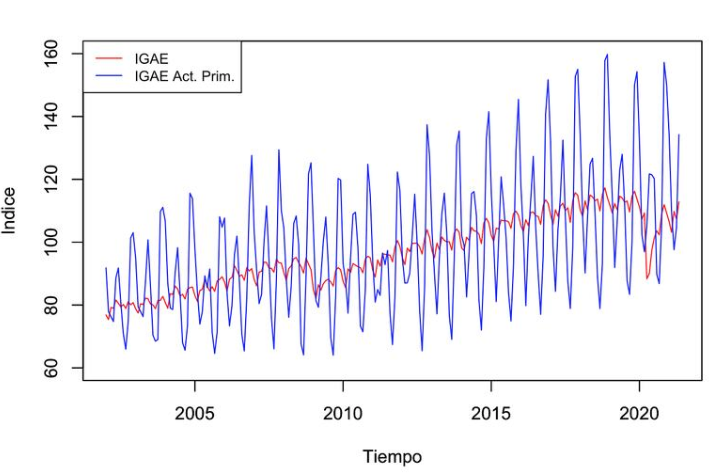
\includegraphics[width=4.16667in,height=3.125in]{Portada.png}

\hypertarget{contexto-del-documento}{%
\section*{Contexto del documento}\label{contexto-del-documento}}
\addcontentsline{toc}{section}{Contexto del documento}

Estas son notas de clase de la materia de Análisis de Series de Tiempo en la Facultad de Economía de la Universidad Nacional Autónoma de México.

Este es un trabajo siempre en proceso de mejora, para cualquier comentario o aclaración, contactar al correo \href{mailto:benjov@ciencias.unam.mx}{\nolinkurl{benjov@ciencias.unam.mx}} o \href{mailto:omarxalpha@gmail.com}{\nolinkurl{omarxalpha@gmail.com}}.

\hypertarget{introducciuxf3n}{%
\chapter{Introducción}\label{introducciuxf3n}}

Estas notas son un resumen, una síntesis comparativa y, en algunos casos, una interpretación propia de los libros de texto de Brooks (2019), Cowpertwait y Metcalfe (2009), Guerrero-Guzmán (2014), Enders (2015), Franses y van Dijk (2003), Kirchgassner, Wolters, y Hassler (2012), Lutkepohl (2005), Wei (2019), entre otros. En algunos casos se incorpora información adicional para efectos de dar contexto al tema analizado (ver sección de Bibliografía para mayores detalles).

El objetivo de este documento es proporcionar un conjunto de apuntes o notas que sirvan de apoyo para la clase de Series de Tiempo en la Facultad de Economía de la UNAM. Por esta razón, no deben considerarse como notas exhaustivas o como un sustituto de la clase y los laboratorios. Asimismo, es deseable que los alumnos puedan aportar sus observaciones y correcciones a estas notas, las observaciones a estas notas son esperadas y siempre serán bienvenidas y agradecidas.

Este es un trabajo siempre en proceso de mejora, para cualquier comentario o aclaración, contactar al correo \href{mailto:benjov@ciencias.unam.mx}{\nolinkurl{benjov@ciencias.unam.mx}} o \href{mailto:omarxalpha@gmail.com}{\nolinkurl{omarxalpha@gmail.com}}.

En estas notas se estudian los temas que típicamente son incluidos como parte de un curso estándar de análisis de series de tiempo y agrega otros tantos, los cuales son:

\begin{enumerate}
\def\labelenumi{\arabic{enumi}.}
\item
  Modelos estacionarios univaraidos: \(AR(p)\), \(MA(q)\), \(ARMA(p, q)\) y \(ARIMA(p, d, q)\), y filtros para eliminar estacionalidad, entre otros;
\item
  Modelos no estacionarios univariados y Pruebas de raíz unitaria (o pruebas para determinar que una serie es estacionaria);
\item
  Modelos multivariados, entre lo que se incluye a los Vectores Autoregresivos (VAR) y los procedimientos de Cointegración
\item
  Modelación de series univariadas con errores con heterocedasticidad y autocorrelación: ARCH(r), GARCH(n), etc.;
\item
  Modelos multivariados con errores con heterocedasticidad y autocorrelación: M-GARCH y M-GARCH-M;
\item
  Casos particulares en los que las series incluidas en un modelo multivariado no son del mismo orden de integración, conocidos como modelos ADRL.
\item
  Modelos de Datos Panel en series de tiempo, y
\item
  Modelos no lineales como los de cambios de régimen.
\end{enumerate}

\hypertarget{la-naturaleza-de-los-datos-de-series-de-tiempo}{%
\section{La naturaleza de los datos de Series de Tiempo}\label{la-naturaleza-de-los-datos-de-series-de-tiempo}}

El análisis de series de tiempo tiene muchas aplicaciones en diversos campos de la ciencia. Por ejemplo, en la economía continuamente se está expuesto a información recopilada de los mercados financieros, indicadores de empleo, índices o indicadores del nivel de producción, índices de precios, etc. En otros campos de las ciencias sociales se emplea el análisis de series de tiempo para analizar la evolución de la población, los nacimientos, o el número de personas con matriculas escolares. Finalmente, en las ciencias exactas se pueden encontrar casos como los de un epidemiólogo que puede estar interesado en el número de casos de influenza observados en algún periodo de tiempo dado y si a estos se les puede asociar con algún tipo de estacionalidad o si se trata del inicio de un fenómeno atípico.

La primera aproximación que se suele tener a las series de tiempo es mediante el examen de datos puestos en una gráfica, en la cual uno de los ejes es el tiempo y el otro es el valor tomado por la variable. No obstante, en este tipo de exámenes existen dos enfoques. Por un lado, existe el efoque de la importancia del tiempo, el cual consiste en reconocer cómo lo que sucede hoy es afectado por lo que pasó ayer o, en general, en periodos pasados, o cómo lo que pasa hoy afectará los eventos futuros. Por otro lado, existe el enfoque del análisis frecuentista o de frecuencia, mediante el cual se busca reconocer la importancia que tiene para los investigadores los ciclos --por ejemplo, ciclos estacionales, momentos de crisis económicas, etc.--

\hypertarget{ejemplos-y-aplicaciones-de-las-series-de-tiempo}{%
\section{Ejemplos y aplicaciones de las Series de Tiempo}\label{ejemplos-y-aplicaciones-de-las-series-de-tiempo}}

Un primer ejemplo que puede ilustrar la presencia de los dos tipos de
enfoques antes mencionadas es la Figura \ref{fig:fig1}. En esta figura se muestra la evolución del Indicador Global de la Actividad Económica (IGAE) en su versión global o del total de la economía y en su versión únicamente para las actividades primarias entre enero de 2002 y mayo de 2023.

\begin{figure}

{\centering 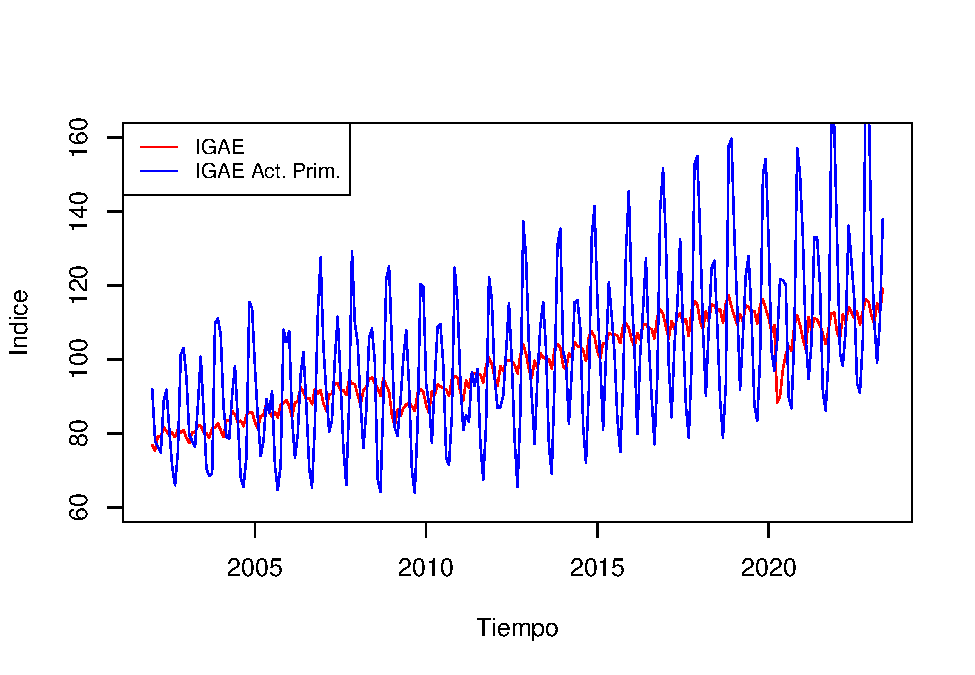
\includegraphics{Notas-Series-Tiempo_files/figure-latex/fig1-1} 

}

\caption{Indicador Global de Actividad Económica (IGAE) Global y para las Actividades Primarias (2008=100), Ene.2002 - May.2023}\label{fig:fig1}
\end{figure}

Como se puede observar, el IGAE del total de la economía muestra, principalmente, que el enfoque del tiempo es más relevante. Es decir, que existe cierta persistencia en el indicador, lo que significa que la economía crece en razón del crecimiento reportado en periodos pasados. No obstante, lo que no podemos reconocer es que los eventos futuros tienen un efecto en el desempeño de la economía hoy día. Así, no es común observar cambios abruptos
del indicador, salvo por la crisis global de 2008 y la reciente crisis causada
por la Covid-19.

\begin{figure}

{\centering 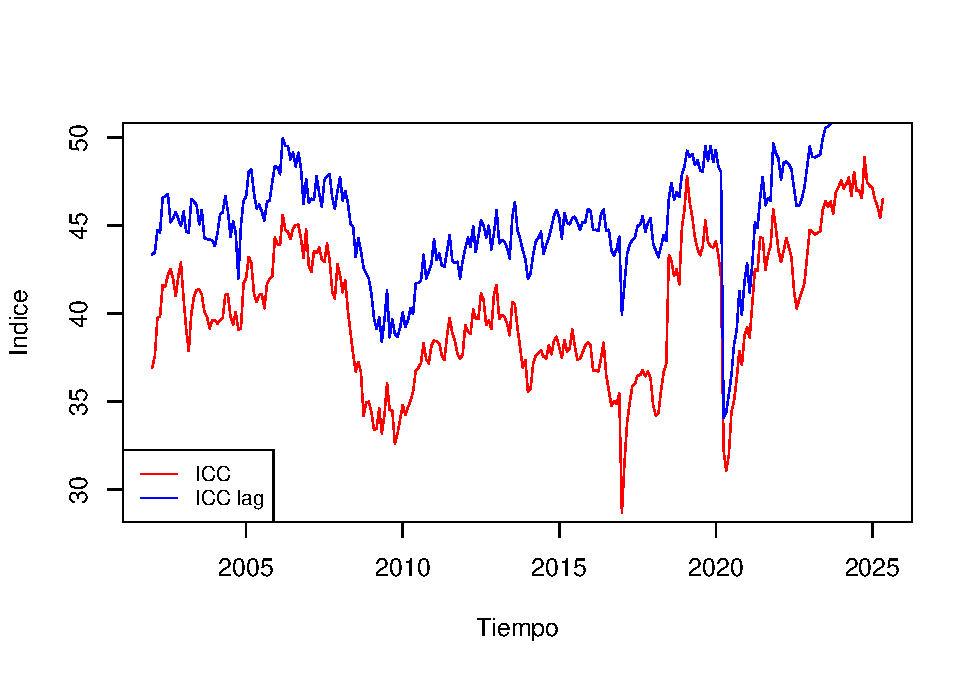
\includegraphics{Notas-Series-Tiempo_files/figure-latex/fig2-1} 

}

\caption{Índice de Confianza del Consumidor (ICC): General y resultado de ¿Cómo considera usted la situación economica del país hoy en día comparada con la de hace 12 meses? (puntos), Ene.2002-may.2023}\label{fig:fig2}
\end{figure}

Por el contrario, el IGAE de las actividades primarias muestra una presencia significativa de la importancia de la frecuencia. No pasa desapercibido que existen muchos ciclos en la evolución del indicador. Algo que suena común
en las actividades primarias, cuya producción depende de eventos que son ciclícos agrícolas asociados con el clima u otros factores determinantes de la oferta de productos agrícolas. Otro factor que puede incluir en el indicador
son elementos de demanda, más que los de oferta. Por ejemplo, el consumo de alimentos típicos de algunas temporadas del año.

Como segundo ejemplo, en la Figura \ref{fig:fig2} se ilustra la evolución reciente del índice de Confianza del Consumidor (ICC) en dos de sus versiones: i) el Índice global y ii) el Índice de confianza de los consumidores cuando estos consideran la situación actual en la economía en relación el año anterior.

Destacamos que el ICC mide las expectativas de los consumidores en razón de la información pasada y de la esperada, segun dichos consumidores.

\begin{figure}

{\centering 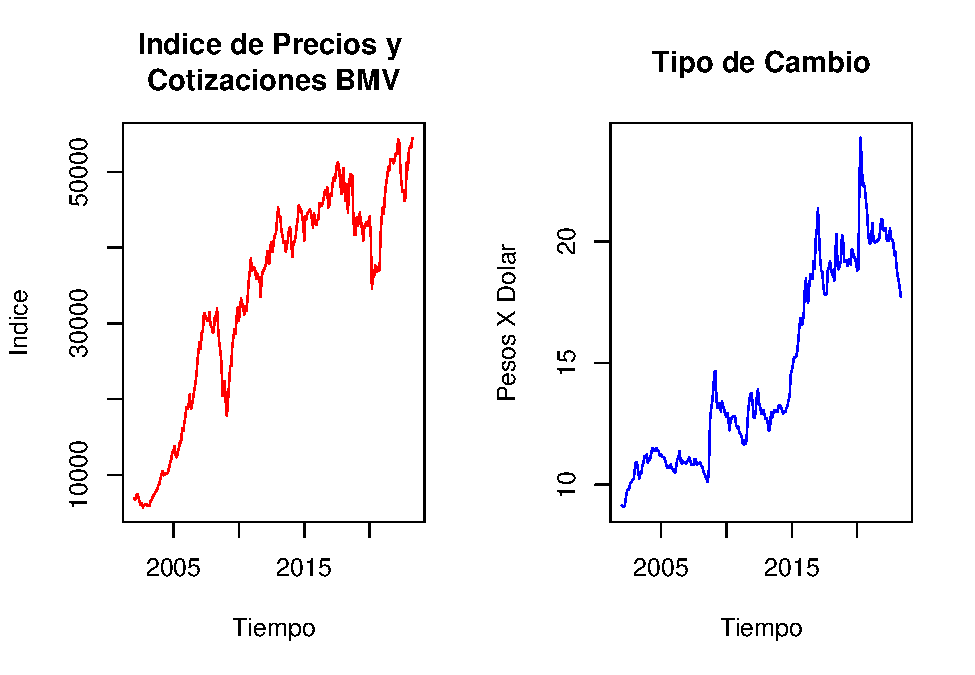
\includegraphics{Notas-Series-Tiempo_files/figure-latex/fig3-1} 

}

\caption{índice de Precios y Cotizaciones de la Bolsa Mexicana de Valores (Panel Derecho) y Tipo de Cambio para Solventar Obligaciones en Moneda Extranjera, pesos por dólar (Panel izquierdo), Ene.2002-May.2023}\label{fig:fig3}
\end{figure}

Así, es probable que las dos series de tiempo exhiban un gran peso para los eventos pasados, pero a la vez, un componente --probablemente menor-- del componente de frecuencia. Esto último en razón de que los consumidores suelen considerar en sus expectativas de consumo los periódos cíclicos de la economía: temporadas navideñaas, pagos de colegiaturas, etc. Este sengundo ejemplo tambien ilustra que la confianza del consumidor no necesariamente está directamente correlacionada con el desempeño de la economía.

Como tercer ejemplo se muestra la evolución de dos series. La Figura \ref{fig:fig3} ilustra el comportamiento reciente de dos indicadores que son referencia para los inversionistas. Por un lado, se ubica el índice de Precios y Cotizaciones de la BMV (IPC), el cuál refleja el valor de las acciones de empresas que cotizan en la BMV y el volumen de acciones comercializadas, en conjunto. De esta forma, se ha interpretado que el IPC refleja el rendimiento del capital promedio invertido en las empresas que cotizan en la BMV.

Por otro lado, en la Figura \ref{fig:fig3} se presenta la evolución del Tipo de Cambio (TDC) --indicador financiero que se suele utilizar como medio de reserva de valor--. Esto, en razón de que el TDC es conocido como un instrumento que en momentos de crisis toma valores contraciclicos de la economía mexicana. No obstante, ambos indicadores no son comparables. Para hacerlos comparbles en la Figura \ref{fig:fig4} se presentan en versión índice con una base en el primer mes de la muestra.

\begin{figure}

{\centering 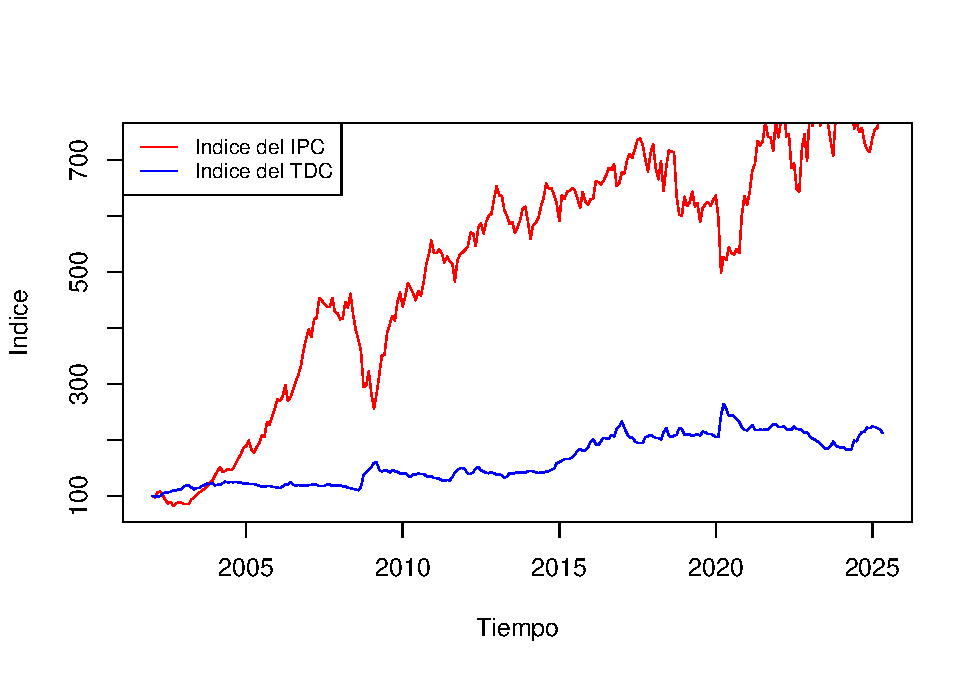
\includegraphics{Notas-Series-Tiempo_files/figure-latex/fig4-1} 

}

\caption{Índice del índice de Precios y Cotizaciones de la Bolsa Mexicana de Valores (Panel Derecho) e Índice del Tipo de Cambio para Solventar Obligaciones en Moneda Extranjera (ambos enero de 2002 = 100), pesos por dólar (Panel izquierdo), Ene.2002-May.2023 }\label{fig:fig4}
\end{figure}

En la perspectiva de la Figura \ref{fig:fig4} se puede apreciar que el TDC no es tan rentable, ya que una inversión en la BMV mediante el IPC, en el largo plazo, muestra más redimientos. Asimismo, la Figura \ref{fig:fig4} ilustra que en ambas series se observa un dominio de la condición de tiempo y no uno de frecuencia. Es decir, tanto el IPC como el TDC no responden a condiciones como ciclos o temporadas que si son observables en actividades económicas como las
primarias.

Finalmente, la Figura \ref{fig:fig5} ilustra un característica que también resulta de gran interés en el analásis de series de tiempo: los datos de alta frecuencia y de comportamiento no regular. Como se puede observar, en la Figura \ref{fig:fig5} se muestran las diferencias logarítmicas de las series de IGAE de la actividad total, el IPC y el TDC.

\begin{figure}

{\centering 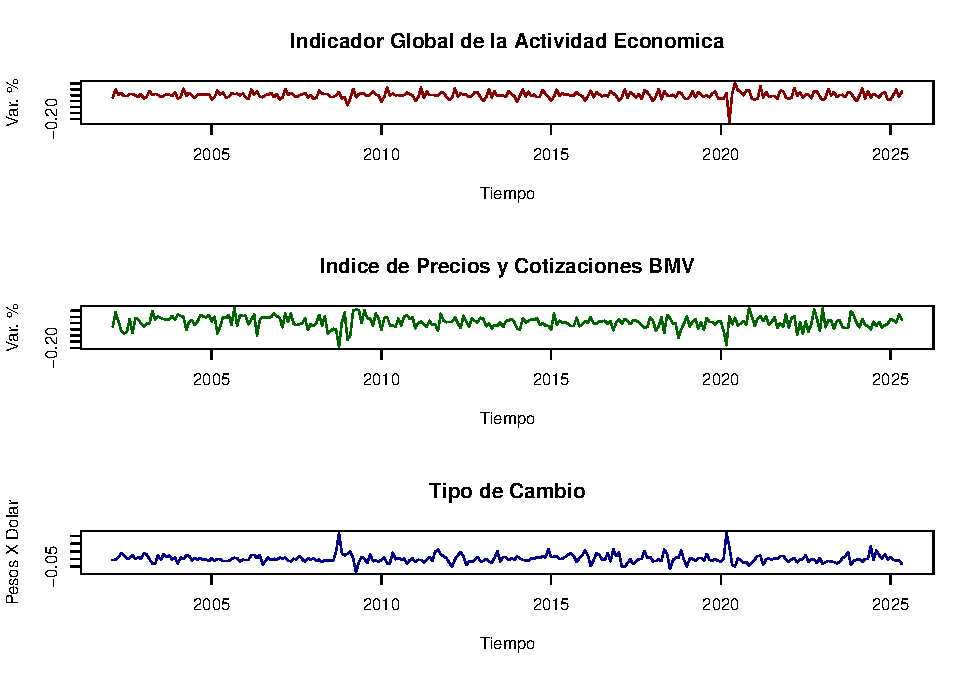
\includegraphics{Notas-Series-Tiempo_files/figure-latex/fig5-1} 

}

\caption{Tasas de Crecimiento mensuales (diferencias logarítmicas) de Indicador Global de la Actividad Económica, Índice de Precios y Cotizaciones de la Bolsa Mexicana de Valores (Panel Derecho) y Tipo de Cambio para Solventar Obligaciones en Moneda Extranjera, Ene.2002-May.2023}\label{fig:fig5}
\end{figure}

Dichas diferencia se pueden interpretar como una tasa de crecimiento de las series por las siguientes razones. Consideremos una serie de tiempo dada por \(y_t\), cuya versión logarítmica es \(ln(y_t\)). De esta forma, la diferencia logarítmica esta dada por la ecuación \eqref{eq:difflog}:

\begin{equation}
   \Delta ln(y_t) = ln(y_t) - ln(y_{t-1}) = ln \left( \frac{y_t}{y_{t-1}} \right)
   \label{eq:difflog}
\end{equation}

Ahora bien, si retomamos la definición de tasa de crecimiento (TC) de una serie de tiempo \(y_t\) entre el periodo \(t\) y \(t-1\) podemos obtener que:

\begin{equation}
    TC = \frac{y_t - y_{t-1}}{y_{t-1}} = \frac{y_t}{y_{t-1}} - 1
    \label{eq:TC}
\end{equation}

De esta forma, si tomamos el logarítmo de la expresión de la ecuación \eqref{eq:TC} obtenemos la siguiente aproximación:

\begin{equation}
    \frac{y_t}{y_{t-1}} -1  \approx ln \left( \frac{y_t}{y_{t-1}} \right) = ln(y_t) - ln(y_{t-1})
    \label{eq:TCDiffLog}
\end{equation}

La ecuación \eqref{eq:TCDiffLog} es cierta cuando los valores de \(y_t\) y \(y_{t-1}\) son muy parecidos, es decir, cuando las variaciones no son tan abruptas. Otra forma de interpretar la ecuación \eqref{eq:TCDiffLog} es que para tasas de crecimiento pequeñas, se puede utilizar como una buena aproximación a la diferencia logarítmica mostrada en la ecuación \eqref{eq:difflog}.

En la Figura \ref{fig:fig5} se reportan las diferencias logarítmicas del IGAE, IPC y TDC, todos, como una media de distitntos tipos de redimientos. Es decir, podemos decir que un capitalista promedio (suponiendo que solo puede invertir en la actividad económica, en la bolsa o en el dólar), puede observar que le es más redituable en función de sus preferencias.

Notése que la dinámica de las variaciones de cada una de las series es significativamente diferente. Destaca que el TDC es una de las variables que, en general, no muestra grandes cambios a lo largo del tiempo. No obstante, se han observado cambios radicales, cuando menos en el año 2008. Lo anterior, son caracteristicas que se han observado para el IPC. En cambio, el IGAE muestra un comportamiento más estable o estacionario.

\hypertarget{elementos-de-ecuaciones-en-diferencia}{%
\chapter{Elementos de Ecuaciones en Diferencia}\label{elementos-de-ecuaciones-en-diferencia}}

\hypertarget{ecuaciones-en-diferencia-para-procesos-deterministas}{%
\section{Ecuaciones en Diferencia para procesos deterministas}\label{ecuaciones-en-diferencia-para-procesos-deterministas}}

En el capítulo previo se hizó una introducción al concepto de series de tiempo. En este Capítulo se pretende desarrollar la construcción de los procesos generadores de datos de las series de tiempo. En un sentido más formal, se expondrá que las series de tiempo se pueden considerar como una secuencia de variables aleatorias.

Para tales efectos, se desarrollará una introducción al concepto de ecuaciones en diferencia. Así, las preguntas que se pretende responder son:

\begin{enumerate}
\def\labelenumi{\arabic{enumi}.}
\item
  ¿Cuál es la solución de la ecuación en diferencia que se estudia?
\item
  ¿Cuáles son las condiciones para que un proceso estocástico, representado mediante una ecuación en diferencia, llegue a alcanzar un punto de equilibrio en el largo plazo?
\end{enumerate}

El término de \emph{ecuación en diferencia} sirve para denominar un proceso similar o equivalente dentro de las ecuaciones diferenciales, dentro del cual se consideran a un conjunto de variables que están en función del tiempo. Así, si consideramos al tiempo como una variable continua, es decir, consideramos una variable \(Z(t)\), podemos expresar las siguientes expresiones para la ecuación diferencial:
\begin{equation}
    \frac{dZ(t)}{dt}; \frac{d^2Z(t)}{dt^2}; \ldots; \frac{d^kZ(t)}{dt^k}
        \label{eq:eqDiff}
\end{equation}

Por otro lado, suponiendo el caso del tiempo en forma discreta, es decir, con \(t = \ldots, -2, -1, 0, 1, 2, \ldots\), entonces el comportamiento de la serie de variables dadas por \(Z_t\), la cual se puede expresar como:
\begin{equation}
    \Delta Z_t; \Delta^2 Z_t; \ldots; \Delta^k Z_t
    \label{eq:Diff1}
\end{equation}

Observemos que una forma técnicamente más correcta es escribir las expresiones anteriores como:
\begin{equation}
    \frac{\Delta Z_t}{\Delta t}; \frac{\Delta^2 Z_t}{\Delta t^2}; \ldots; \frac{\Delta^k Z_t}{\Delta t^k}
    \label{eq:Diff2}
\end{equation}

No obstante, no pasa desapercibido que \(\Delta t = 1\), por lo que resultan equivalentes ambos conjuntos de expresiones \eqref{eq:Diff1} y \eqref{eq:Diff2}.

\hypertarget{ecuaciones-en-diferencia-lineales-de-primer-orden}{%
\subsection{Ecuaciones en Diferencia Lineales de Primer Orden}\label{ecuaciones-en-diferencia-lineales-de-primer-orden}}

El primer caso que se suele estudiar en relación a Ecuaciones en Diferencia es el de las Ecuaciones en Diferencia Lineales de Primer Orden. Al respecto, al igual que en el caso continúo, las variaciones de la variable \(Z_t\) se pueden expresar como se ilustra en el siguiente ejemplo. Consideremos la siguiente ecuación:
\begin{equation}
    Z_t = a_0 + a_1 Z_{t-1}
    \label{eq:EDPO}
\end{equation}

Donde, \(t = \ldots, -2, -1, 0, 1, 2, \ldots\), y \(a_0\) y \(a_1 \neq 0\) son números reales constantes. De \eqref{eq:EDPO} podememos despejar la variable \(Z_{t-1}\) y obtener una forma de ecuación en diferencia:
\begin{equation}
    Z_t - a_1 Z_{t-1} = a_0
    \label{eq:EDPO2}
\end{equation}

Ahora denotemos a \(L Z_t = Z_{t-1}\), es decir, mediante el operador \(L\) se puede rezagar una variable dada. En general, podemos decir que el operador tiene dos propiedades, la primera es que es lineal en el sentido de que abre sumas y saca escalares como se muestra en la siguiente expresión para el caso de un (1) rezago:
\begin{equation}
    L(\alpha Z_{t} + \beta) = \alpha Z_{t-1} + \beta
    \label{eq:E1Lag}
\end{equation}

Donde \(\alpha, \beta \in \mathbb{R}\) y \(\alpha, \beta \neq 0\). Otro reesultado implícito en esta primera propiedad es que el operador rezago aplicado a cualquier escalar dará como resultado el escalar, puesto que este es una constante sin importa el momento \(t\) en el cual se encuentre la variable \(Z\).

La segunda propiedad del operador es que se puede aplicar de forma consecutiva a una misma variable. Es decir, \(L ( Z_{t-1}) = L L Z_{t} = L^2 Z_{t}\), por lo que en general tendremos: \(L^p Z_t = Z_{t-p}\) (con \(p \in \mathbb{Z}\)). Así, en el caso de \(p\) rezagos la propiedad de linealidad del operador rezago será:
\begin{equation}
    L^p (\alpha Z_{t} + \beta) = \alpha Z_{t-p} + \beta
   \label{eq:LinProp}
\end{equation}

Dicho lo anterio podemos escribir la solución general de \eqref{eq:EDPO2} como:
\begin{eqnarray}
    Z_t - a_1 L Z_t & = & a_0 \nonumber \\
    (1 - a_1 L)Z_t & = & a_0 \nonumber \\
    Z_t & = & a_0 \frac{1}{1 - a_1 L} + s a^t_1 \nonumber \\
    Z_t & = & a_0 \frac{1}{1 - a_1} + s a^t_1
    \label{eq:PROC01}
\end{eqnarray}

Donde \(a_1 \neq 1\) y \(t = \ldots, -2, -1, 0, 1, 2, \ldots\). Notése que la aplicación del operador rezago \(L\) a la constante \(a_1\) dará como resultado el valor de la misma constante, ya que ésta no depende del momento \(t\) en el cuál observemos a la variable \(Z_t\). En la ecuación \eqref{eq:PROC01} se adiciona un término \(s a^t_1\) que permite ubicar la trayectoria inicial de la solución de la ecuación. El componente no significa un cambio respecto de la ecuación \eqref{eq:EDPO2} original, ya que si buscaramos reconstruir a ésta ecuación tendríamos:
\begin{eqnarray}
    (1 - a_1 L) s a^t_1 & = & s a^t_1 - a_1 s L a^{t}_1 \nonumber \\
    & = & s a^t_1 - a_1 s a^{t - 1}_1 \nonumber \\
    & = & s a^t_1 - s a^t_1 \nonumber \\
    & = & 0 \nonumber
\end{eqnarray}

La ecuación \eqref{eq:PROC01} se suele interpretar como la solución de largo plazo. Ahora demostraremos por qué es cierta la ecuación y discutiremos algunas condiciones que se deben observar en esta solución para que sea una solución convergente. No obstante, primero discutiremos un método indirecto e incompleto para demostrar el resultado, dicho método es conocido como el método iterativo. Plantearemos las siguientes ecuaciones partículares donde suponemos la existencia del valor inicial \(Z_0\) del proceso:
\begin{equation*}
    Z_1 = a_0 + a_1 Z_0
\end{equation*}

\begin{eqnarray*}
Z_2 & = & a_0 + a_1 Z_1 \\
    & = & a_0 + a_1 (a_0 + a_1 Z_0) \\
    & = & a_0 +  a_0 a_1 + a^2_1 Z_0 \\
    & = & a_0 (1 + a_1) + a^2_1 Z_0
\end{eqnarray*}

\begin{eqnarray*}
Z_3 & = & a_0 + a_1 Z_2 \\
    & = & a_0 + a_1 (a_0 +  a_0 a_1 + a^2_1 Z_0) \\
    & = & a_0 +  a_0 a_1 + a_0 a^2_1 + a^3_1 Z_0 \\
    & = & a_0 (1 + a_1 + a^2_1) + a^3_1 Z_0
\end{eqnarray*}

De lo anterior se puede inferir que el método iterativo convergerá hacia una expresión como la siguiente en el momento \(t\):
\begin{eqnarray}
Z_t & = & a_0 + a_1 Z_{t-1} \nonumber \\
    & = & a_0 (1 + a_1 + a^2_1 + \ldots + a^{t-1}_1) + a^t_1 Z_0 \nonumber \\
    & = & a_0 \sum^{t-1}_{i = 0}{a^i_1} + a^t_1 Z_0
    \label{eq:SUM}
\end{eqnarray}

Donde, es necesario que en la ecuación \eqref{eq:SUM} se cumpla que \(\lvert{a_1}\lvert < 1\) para que la suma sea convergente --más adelante detallaremos esta afirmación--. A este tipo de ecuaciones se les puede denominar como lineales. Esto en razón de que ningún término de la variable \(Z\) aparce elevado a ninguna potencia distinta a 1. También, son de primer orden, ya que el rezago de la variable \(Z\) es sólo de un período.

En adelante trabajaremos con ecuaciones en las que la variable \(Z\) se encuentra rezagada en cualquiera de los siguientes casos:
\begin{equation}
    Z_t, Z_{t-1}, Z_{t-2}, Z_{t-3}, \ldots, Z_{t-p}, \ldots
    \label{eq:SUM0}
\end{equation}

Por lo que diremos que en adelante el curso versará sobre ecuaciones en diferencia lineales y de cualquier orden \(p\).

Retomando la ecuación \eqref{eq:SUM} y considerando la parte de la suma de los términos de \(a^i_1\), de tal forma que buscaremos dar una expresión más compresible a dicho término. Definamos la siguiente expresión como:
\begin{equation}
    S_{t-1} = \sum^{t-1}_{i = 0}{a^i_1}
    \label{eq:St1}
\end{equation}

Por lo tanto, \(S_t\) estaría dado por la siguiente expresión:
\begin{eqnarray}
S_{t} & = & a_1 \sum^{t-1}_{i = 0}{a^i_1} \nonumber \\
      & = & a_1 (1 + a_1 + a^2_1 + \ldots + a^{t-1}_1) \nonumber \\
      & = & a_1 + a^2_1 + a^3_1 + \ldots + a^{t}_1 \nonumber \\
      & = & a_1 S_{t-1}
      \label{eq:St}
\end{eqnarray}

Tomando los dos resultados de las ecuaciones \eqref{eq:St1} y \eqref{eq:St} anteriores, podemos expresar que si a \(S_{t-1}\) le restamos \(S_t\), y desarrollando ambos lados de la ecuación anterior podemos obtener:
\begin{eqnarray}
    S_{t-1} - a_1 S_{t-1} & = & S_{t-1} - S_{t} \nonumber \\
    (1 - a_1) S_{t-1} & = & (1 + a_1 + a^2_1 + \ldots + a^{t-1}_1) - (a_1 + a^2_1 + a^3_1 + \ldots + a^{t}_1) \nonumber \\
    (1 - a_1) S_{t-1} & = & 1 - a^{t}_1 \nonumber
\end{eqnarray}

Así, podemos concluir que:
\begin{equation}
    S_{t-1} = \frac{1 - a^{t}_1}{1 - a_1}
    \label{eq:SUM2}
\end{equation}

Conjuntando éste último resultado de la ecuación \eqref{eq:SUM2} con la ecuación \eqref{eq:SUM} tenemos la siguiente solución por el método de iteración:
\begin{equation}
    Z_t = a_0 \left( \frac{1 - a^{t}_1}{1 - a_1} \right) + a^t_1 Z_0
    \label{eq:SOLITER}
\end{equation}

De esta forma la ecuación \eqref{eq:SOLITER} es una solición para la ecuación \eqref{eq:SUM}, que es una ecuación de un proceso de una Ecuación en Diferencia plantenado en la ecuación \eqref{eq:EDPO}. Está solución aún no es general, en el sentido de que sea válida para cualquiel tipo de proceso: convergente o divergente. Dicha convergencia o divengencia estará determinada por el paramétro \(a_1\). No debe pasar desapercibido que cuando \(t \rightarrow \infty\) o cuando la muestra es muy grande (lo que es equivalente), podemos decir que la solución solo puede converger a la siguiente expresión cuando se considera que \(|a_1| < 1\):
\begin{equation}
    Z_t = a_0 \left( \frac{1}{1 - a_1} \right)
    \label{eq:trayec}
\end{equation}

Retomemos ahora el caso general descrito en la ecuación \eqref{eq:PROC01} y determinemos una solución general en la cual \(a_1 \neq 1\) y \(t = \ldots, -2, -1, 0, 1, 2, \ldots\). Para ello observemos que el siguiente componente en la ecuación mencionada se puede interpretar como la suma infinita de términos descritos como:
\begin{eqnarray}
    \frac{1}{1 - a_1} & = & 1 + a_1 + a_1^2 + \ldots + a_1^t + \ldots \nonumber \\
    & = & \sum_{i = 0}^{\infty} a_1^{i}
    \label{eq:SUMINF}
\end{eqnarray}

Donde claramente es necesario que \(|a_1| < 1\). Por lo tanto, sólo faltaría determinar el valor de la constante \(s\) en la ecuación \eqref{eq:PROC01} de la siguiente forma, supongamos que observamos el proceso en el momento inicial, por lo que es posible determinar el valor de la constante conociendo el valor inicial del proceso como sigue:
\begin{equation}
    Z_0 = a_0 \frac{1}{1 - a_1} + s
\label{eq:Z0}
\end{equation}

De la ecuación \eqref{eq:Z0} tenemos que:
\begin{equation}
    s = Z_0 - a_0 \frac{1}{1 - a_1}
\label{eq:eqs}
\end{equation}

Así, juntando la ecuación \eqref{eq:PROC01} y ecuación \eqref{eq:eqs} tenemos la expresión:
\begin{equation}
    Z_t = a_0 \frac{1 - a^t_1}{1 - a_1} + a^t_1 Z_0
\label{eq:SOLGEN}
\end{equation}

No debe pasar desapercibido que está solución es la misma que la mostrada en la ecuación (\eqref{eq:SOLITER}, por lo que en realidad ambas ecuaciones son una solución general indistintamente entre las ecuaciones \eqref{eq:SOLITER} y \eqref{eq:SOLGEN}. Ambas convergen a la expresión como la ecuación \eqref{eq:trayec}, con la misma condición de convergencia \(|a_1| < 1\). Para ilustrar estas ecuaciones veámos algunos ejemplos al respecto.

Consideremos que tenemos un proceso \(Z_t\) que es descrito por una ecuación en diferencia lineal de primer orden dada por:
\begin{equation}
    Z_t = 2 + 0.9 Z_{t-1}
\label{eq:ex1}
\end{equation}

Siguiendo la expresión mostrada en la ecuación \eqref{eq:SOLGEN}, obtenemos la expresión:
\begin{equation}
    Z_t = 2 \left( \frac{1 - 0.9^{t}}{1 - 0.9} \right) + 0.9^t Z_0
\label{eq:ex2}
\end{equation}

Donde asumiremos que el valor inicial es \(Z_0 = 10\) y que la expresión debe converger al valor de 20, cuando \(t\) es muy grande o tiende a infinito. De forma similar tomemos otro ejemplo, en el cual asumimos la siguiente expresión:
\begin{equation}
    Z_t = 2 - 0.5 Z_{t-1}
\label{eq:ex3}
\end{equation}

Siguiendo la expresión mostrada en la ecuación \eqref{eq:SOLGEN}, obtenemos:
\begin{equation}
    Z_t = 2 \left( \frac{1 - (-0.5)^{t}}{1 + 0.5} \right) + (-0.5)^t Z_0
\label{eq:ex4}
\end{equation}

Donde asumiremos que el valor inicial es \(Z_0 = 10\) y que la ecuación converge al valor de \(1.3333333 \ldots\), cuando \(t\) es muy grande o tiende a infinito. Ahora simulemos el comportamiento de ambos procesos y estableceremos los resultados del Cuadro \ref{tab:table1}. Notemos que el segundo proceso converge de una forma más rapida que el primero. El Cuadro \ref{tab:table1} se ilustra en las siguientes dos Figura \ref{fig:fig21} y Figura \ref{fig:fig22}.

\hypertarget{ecuaciones-en-diferencia-lineales-de-segundo-orden-y-de-orden-superior}{%
\subsection{Ecuaciones en Diferencia Lineales de Segundo Orden y de orden superior}\label{ecuaciones-en-diferencia-lineales-de-segundo-orden-y-de-orden-superior}}

Como un segundo caso a estudiar se ubica el caso de las Ecuaciones en Diferencia Lineales de Segundo Orden y de orden superior. Primero, sea una ecuación como la siguiente, la cual es lineal y de segundo orden, ya que tiene asociado un término de \(Z_t\) rezagado dos periódos:
\begin{equation}
    Z_t = a_0 + a_1 Z_{t-1} + a_2 Z_{t-2}
    \label{eq:EDSO}
\end{equation}

Table: \label{tab:foo} Dos ejemplos de procesos de Ecuaciones Lineales de Primer Orden convengentes

\begin{longtable}[]{@{}rrr@{}}
\caption{\label{tab:table1}Dos ejemplos de Procesos de Ecuaciones Lineales de Primer Orden Convergentes}\tabularnewline
\toprule\noalign{}
Tiempo & \(Z_t =2+0.9Z_{t-1}\) & \(Z_t = 2-0.5Z_{t-1}\) \\
\midrule\noalign{}
\endfirsthead
\toprule\noalign{}
Tiempo & \(Z_t =2+0.9Z_{t-1}\) & \(Z_t = 2-0.5Z_{t-1}\) \\
\midrule\noalign{}
\endhead
\bottomrule\noalign{}
\endlastfoot
0 & 10.00000 & 10.000000 \\
1 & 11.00000 & -3.000000 \\
2 & 11.90000 & 3.500000 \\
3 & 12.71000 & 0.250000 \\
4 & 13.43900 & 1.875000 \\
5 & 14.09510 & 1.062500 \\
6 & 14.68559 & 1.468750 \\
7 & 15.21703 & 1.265625 \\
8 & 15.69533 & 1.367188 \\
9 & 16.12580 & 1.316406 \\
10 & 16.51322 & 1.341797 \\
11 & 16.86189 & 1.329102 \\
12 & 17.17570 & 1.335449 \\
13 & 17.45813 & 1.332275 \\
14 & 17.71232 & 1.333862 \\
15 & 17.94109 & 1.333069 \\
96 & 19.99960 & 1.333333 \\
97 & 19.99964 & 1.333333 \\
98 & 19.99967 & 1.333333 \\
99 & 19.99970 & 1.333333 \\
100 & 19.99973 & 1.333333 \\
\end{longtable}

\begin{figure}

{\centering 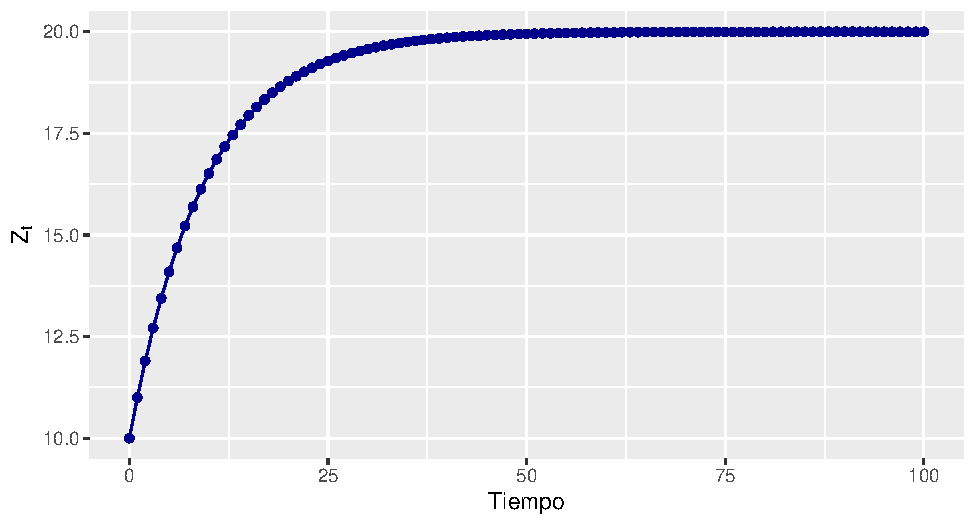
\includegraphics{Notas-Series-Tiempo_files/figure-latex/fig21-1} 

}

\caption{Evolución del proceso dado por $Z_t =2+0.9Z_{t-1}$}\label{fig:fig21}
\end{figure}

\begin{figure}

{\centering 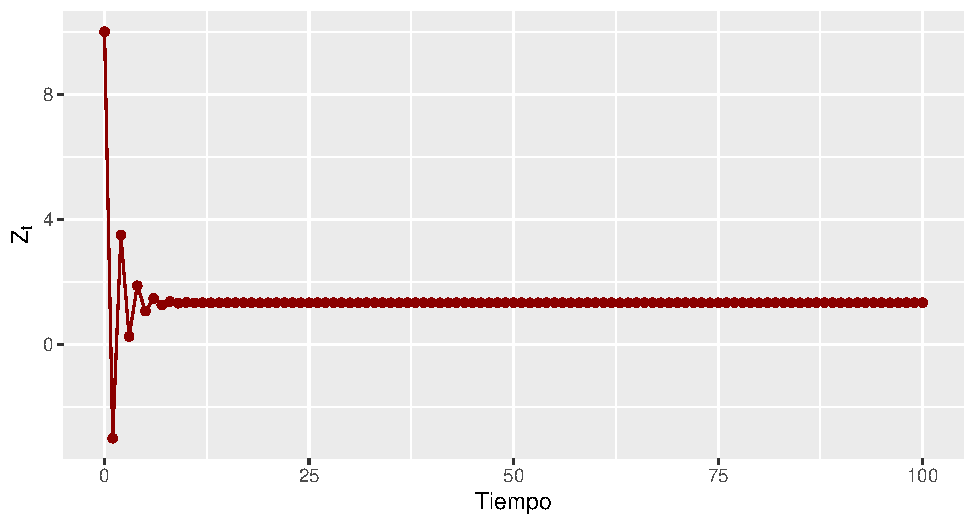
\includegraphics{Notas-Series-Tiempo_files/figure-latex/fig22-1} 

}

\caption{Evolución del proceso dado por $Z_t =2-0.5Z_{t-1}$}\label{fig:fig22}
\end{figure}

Donde \(t = \ldots, -2, -1, 0, 1, 2, \ldots\) y \(a_1, a_2 \neq 0\). Reordenando la ecuación \eqref{eq:EDSO} podemos escribir:
\begin{eqnarray}
    Z_t - a_1 Z_{t-1} - a_2 Z_{t-2} & = & a_0 \nonumber \\
    Z_t - a_1 L Z_{t} - a_2 L^2 Z_{t} & = & a_0 \nonumber \\
    (1 - a_1 L - a_2 L^2)Z_t & = & a_0 
    \label{eq:EDSOSOL}
\end{eqnarray}

Así, la solución general propuesta para la ecuación \eqref{eq:EDSOSOL} es la siguiente, la cual es una forma analóga a una Ecuación Lineal en Diferencia de Primer Orden:
\begin{equation}
    Z_t = \frac{a_0}{1 - a_1 - a_2} + s_1 g^t_1 + s_2 g^t_2
    \label{eq:SOLGEN2}
\end{equation}

En donde \(s_1\) y \(s_2\) son constantes que se determinan mediante dos condiciones iniciales --por lo que para resolver este tipo de ecuaciones requerimos conocer dos condiciones iniciales--. Los valores de \(g_1\) y \(g_2\) están relacionados con los coeficientes \(a_1\) y \(a_2\), de esta forma:
\begin{equation}
  a_1  =  g_1 + g_2
  \label{eq:a1}
\end{equation}

\begin{equation}
    a_2  =  - g_1 g_2
    \label{eq:a2}
\end{equation}

Lo anterior surge del siguiente procedimiento y recordando que siempre es posible descomponer una ecuación cuadrática en expresiones como las siguientes:
\begin{eqnarray}
    (1 - a_1 L - a_2 L^2) & = & (1 - g_1 L)(1 - g_2 L) \nonumber \\
    & = & 1 - g_1 L - g_2 L + g_1 g_2 L^2 \nonumber \\
    & = & 1 - (g_1 + g_2) L + g_1 g_2 L^2
    \label{eq:eqcaracteristica}
\end{eqnarray}

Donde se observa la equivalencia mostrada en las ecuaciones \eqref{eq:a1} y \eqref{eq:a2}. Así, considerando la ecuación \eqref{eq:SOLGEN2} tenemos que:
\begin{eqnarray}
    (1 - a_1 L - a_2 L^2) Z_t & = & (1 - g_1 L)(1 - g_2 L) Z_t \nonumber \\
    & = & a_0 + (1 - g_1 L)(1 - g_2 L) s_1 g^t_1 \nonumber \\
    &  & + (1 - g_1 L)(1 - g_2 L) s_2 g^t_2
    \label{eq:eqcaracteristica1}
\end{eqnarray}

Por lo tanto, buscamos que para que el proceso sea equivalente y podamos interpretar que la ecuación \eqref{eq:SOLGEN2} sea una solución general deberá pasar lo siguiente:
\begin{equation}
    (1 - g_1 L) (1 - g_2 L) s_1 g^t_1 + (1 - g_1 L) (1 - g_2 L) s_2 g^t_2 = 0
    \label{eq:eqcaracteristica2}
\end{equation}

O, escrito de otra forma:
\begin{equation}
    (1 - g_1 L) s_1 g^t_1 = (1 - g_2 L) s_2 g^t_2 = 0
    \label{eq:eqcaracteristica3}
\end{equation}

Ahora determinemos cuáles son los valores \(g_1\) y \(g_2\) dados los valores \(a_1\) y \(a_2\) que nos permitan determinar si el proceso será convergente. Para ello debemos resolver la siguiente ecuación que se deriva de la ecuación \eqref{eq:eqcaracteristica}:
\begin{equation}
    1 - a_1 x - a_2 x^2 = (1 - g_1 x)(1 - g_2 x) = 0
    \label{eq:eqcaracteristica4}
\end{equation}

Donde, claramente existen dos raíces: \(x_1 = g^{-1}_1\) y \(x_2 = g^{-1}_2\). Así, la solución estará dada por las raíces de la ecuación característica:
\begin{eqnarray}
    1 - a_1 x - a_2 x^2 = 0 \nonumber \\
    a_2 x^2 + a_1 x - 1 = 0
    \label{eq:POL2}
\end{eqnarray}

Cuya solución es:
\begin{equation}
    x = \frac{- a_1 \pm \sqrt{a^2_1 + 4 a_2}}{2 a_2}
    \label{eq:eqcaracteristica5}
\end{equation}

Es importante distinguir tres diferentes casos en relación con las raíces que surgen como solución de la ecuación \eqref{eq:POL2}, estos son:

\textbf{Caso I}. Si \(a^2_1 + 4 a_2 > 0\), la ecuación \eqref{eq:POL2} proporcionará dos valores de raíces reales y distintos, eso es \(x_1 = g^{-1}_1 \neq x_2 = g^{-1}_2\). Si por ahora suponemos que \(|{g_1} < 1|\) y que \(|{g_2} < 1|\), entonces tendremos que:
\begin{eqnarray}
    (1 - g_1 L)^{-1} (1 - g_2 L)^{-1} a_0 & =&  \left( \sum^{\infty}_{j = 0}{g^j_1 L^j} \right) \left( \sum^{\infty}_{j = 0}{g^j_2 L^j} \right) a_0 \nonumber \\
    & = & \left( \sum^{\infty}_{j = 0}{g^j_1} \right) \left( \sum^{\infty}_{j = 0}{g^j_2} \right) a_0 \nonumber \\
    & = & \frac{a_0}{(1 - g_1)(1 - g_2)} \nonumber \\
    & = & \frac{a_0}{1 - a_1 - a_2}
    \label{eq:eqcaracteristica6}
\end{eqnarray}

Esto último es el punto de equilibrio de la ecuación \eqref{eq:SOLGEN2}; considerando que \(|{g_1} < 1|\) y que \(|{g_2} < 1|\) --notemos que los demás casos son divergentes, ya que la suma anterior nno connvergería--. De esta forma la solución de la ecuación estará dada por:
\begin{equation}
    \lim_{t \to \infty} Z_t = \frac{a_0}{1 - a_1 - a_2}
    \label{eq:Conver}
\end{equation}

\textbf{Caso II}. Si \(a_1^2 + 4a_2 < 0\) en la ecuación \eqref{eq:POL2}, entonces las raíces serán números complejos conjugados, es decir:
\begin{equation}
g_i^{-1}=a \pm ib
\label{eq:Conver1}
\end{equation}

\begin{eqnarray}
    g_i  =  u \pm iv 
    \label{eq:Conver2}
\end{eqnarray}

Dichas raíces las podemos escribir en coordenadas polares como:
\begin{eqnarray}
    g_1^{-1} = r e^{i \theta} = r (cos(\theta) + i sen(\theta))
    \label{eq:Conver3}
\end{eqnarray}
\begin{eqnarray}
    g_2^{-1}  =  r e^{-i \theta} = r (cos(\theta) - i sen(\theta))
    \label{eq:Conver4}
\end{eqnarray}
Donde: \(r = \sqrt{u^2 + v^2}\), a esta expresión también se le conoce como modulo. Alternativamente, podemos escribir que \(r = \sqrt{g_1 g_2}\). La única condición es que \(r < 1\) para que el proceso descrito en la ecuación \eqref{eq:SOLGEN2} sea convergente.

Al igual que en el \textbf{Caso I}, el punto de equilibrio de la ecuación se debería ubicar al rededor \eqref{eq:Conver}, siempre que \(r < 1\), por lo que el factor que determina la convergencia es el modulo, ya que si el modulo es mayor a 1, el proceso será divergente, pero si es menor a 1 convergerá a \eqref{eq:Conver}. Para ilustrar, el caso contrario es divergente puesto que representa trayentorias senoidales (oscilatorias) que sólo pueden converger si a medida que pasa el tiempo, las ondas son menos amplias.

\textbf{Caso III}. Ahora revisemos el caso en el que \(a_1^2 + 4a_2 = 0\), de esta forma las raíces serán identicas:
\begin{equation}
    g = g_1^{-1} = g_2^{-1} = \frac{-a_1}{2 a_2}
    \label{eq:Conver6}
\end{equation}

Así, el punto de equilibrio será dado por la solución descrita como:
\begin{eqnarray}
    (1 - g L)^2 Z_t & = & a_0 \nonumber \\
    Z_t & = & \frac{a_0}{(1 - g L)^2} + s_1 g^t + s_2 t g^t \nonumber \\
    & = & a_0 \sum_{i = 0}^{\infty} (1 + i) g^j + s_1 g^t + s_2 t g^t
    \label{eq:Conver7}
\end{eqnarray}

Donde la expresión amnterior es resultado de considerar el siguiente procedimiento. Sea:
\begin{eqnarray}
    f(g) & = & \frac{1}{(1 - g)} = \sum_{j = 0}^{\infty} g^j \nonumber
\end{eqnarray}

Por lo que si hacemos la primer derivada del la expresión anterior tenemos que:
\begin{eqnarray}
    f'(g) & = & \frac{1}{(1 - g)^2} \nonumber \\
    & = & \sum_{j = 0}^{\infty} j g^{j-1} \nonumber \\
    & = & 0 + g^0 + 2 g^1 + 3 g^2 + \ldots \nonumber \\
    & = & \sum_{j = 0}^{\infty} (1 + j) g^j \nonumber
\end{eqnarray}

Ahora veámos un ejemplo de una Ecuación Lineal en Diferencia de Segundo Orden. Supongamos la ecuación y el desarrollo siguientes:
\begin{eqnarray}
    Z_t & = & 3 + 0.9 Z_{t-1} - 0.2 Z_{t-2} \nonumber \\
    (1 - 0.9 L + 0.2 L^2) Z_t & = & 3 \nonumber
\end{eqnarray}

La solución dada por una ecuación similar a la expresión \eqref{eq:POL2}, obtendríamos la solución dada por las ecuaciones equivalentes a:
\begin{eqnarray}
    1 - 0.9 x + 0.2 x^2 = 0 \nonumber \\
    - 0.2 x^2 + 0.9 x - 1 = 0 \nonumber
\end{eqnarray}

De donde las raíces del polinomio característico \(x_1 = g_1^{-1}\) y \(x_2 = g_2^{-1}\) se obtienen de la expresión dada por:
\begin{eqnarray}
    x & = &\frac{-0.9 \pm \sqrt{0.81 + (4)(-0.2)}}{(2)(-0.2)} \nonumber \\
    & = & \frac{0.9 \pm 0.1}{0.4} \nonumber
\end{eqnarray}

Dado que el componente \(a^2_1 + 4 a_2\) es positivo, obtendremos dos raíces reales. Las raíces estarán dadas por \(x_1 = 2.5\) y \(x_2 = 2.0\), de lo cual podemos determinar que \(g_1 = 0.4\) y \(g_2 = 0.5\). De esta forma tenemos que \(|g_1| < 1\) y \(|g_2| < 1\), así la ecuación converge a la expresión dada por las siguientes expresiones:
\begin{eqnarray}
    Z_t & = & \frac{3}{1 - 0.9 L + 0.2 L^2} + s_1 (0.4)^t + s_2 (0.5)^t \nonumber \\
    & = & \frac{3}{1 - 0.9 + 0.2} + s_1 (0.4)^t + s_2 (0.5)^t \nonumber \\
    & = & \frac{3}{(1 - 0.4)(1 - 0.5)} + s_1 (0.4)^t + s_2 (0.5)^t \nonumber
\end{eqnarray}

Al final, la ecuación que describe la solución general será:
\begin{equation}
    z_t = 10 + s_1 (0.4)^t + s_2 (0.5)^t
    \label{eq:Conver9}
\end{equation}

Para determinar los valores de \(s_1\) y \(s_2\) necesitamos obtener dos valores iniciales de la ecuación para lo cual iniciaremos como \(t = 0\) y luego obtenemos el valor de \(t = 1\), consideremos el valor de \(Z_0 = 0\) y \(Z_1 = 50\):
\begin{eqnarray*}
    Z_0 & = & 10 + s_1(0.4)^0  + s_2(0.5)^0 \\
    0 & = & 10 + s_1 + s_2 \\
    Z_1 & = & 10 + s_1(0.4)^1  + s_2(0.5)^1 \\
    50 & = & 10 + 0.4 s_1 + 0.5 s_2
\end{eqnarray*}

Por lo que la solución es: \(s_1 = -450\) y \(s_2 = 440\), de donde podemos expresar la ecuación como:
\begin{equation}
    Z_t = 10 - 450(0.4)^t + 440(0.5)^t
\label{eq:Ejem01}
\end{equation}

La ecuación \eqref{eq:Ejem01} anterior convergerá al valor de 10 cuando \(t \rightarrow \infty\). Para ilustrar la trayectoria de esta ecuación tomemos un cuadro similar al de los ejemplos anteriores. En el Cuadro \ref{tab:table2} y la Figura \ref{fig:fig23} mostramos los resultados de la trayectorua para 100 periodos.

Finalmente, discutiremos la solución para las Ecuaciones Lineales en Diferencia de Orden \(p\), donde \(p \geq 2\). En general una ecuación de este tipo se puede escribir como:
\begin{equation}
    Z_t = a_0 + a_1 Z_{t-1} + a_2 Z_{t-2} + \ldots + a_p Z_{t-p}
    \label{eq:EDOP}
\end{equation}

Donde \(t = \ldots, -2, -1, 0, 1, 2, \ldots\) y \(a_p \neq 0\). La ecuación \eqref{eq:EDOP} se puede escribir como:
\begin{eqnarray}
    Z_t - a_1 Z_{t-1} - a_2 Z_{t-2} - \ldots - a_p Z_{t-p} & = & a_0 \nonumber \\
    Z_t - a_1 L Z_t - a_2 L^2 Z_t - \ldots - a_p L^p Z_t & = & a_0 \nonumber \\
    (1 - a_1 L - a_2 L^2 - \ldots - a_p L^p) Z_t & = & a_0
    \label{eq:EDOP2}
\end{eqnarray}

\begin{longtable}[]{@{}rr@{}}
\caption{\label{tab:table2}Un ejemplo de proceso de Ecuación de Segundo Orden convengente}\tabularnewline
\toprule\noalign{}
Tiempo & \(Z_t =10-450(0.4)^t+440(0.5)^t\) \\
\midrule\noalign{}
\endfirsthead
\toprule\noalign{}
Tiempo & \(Z_t =10-450(0.4)^t+440(0.5)^t\) \\
\midrule\noalign{}
\endhead
\bottomrule\noalign{}
\endlastfoot
0 & 0.00000 \\
1 & 50.00000 \\
2 & 48.00000 \\
3 & 36.20000 \\
4 & 25.98000 \\
5 & 19.14200 \\
6 & 15.03180 \\
7 & 12.70022 \\
8 & 11.42384 \\
9 & 10.74141 \\
10 & 10.38250 \\
11 & 10.19597 \\
12 & 10.09987 \\
13 & 10.05069 \\
14 & 10.02565 \\
15 & 10.01294 \\
96 & 10.00000 \\
97 & 10.00000 \\
98 & 10.00000 \\
99 & 10.00000 \\
100 & 10.00000 \\
\end{longtable}

\begin{figure}

{\centering 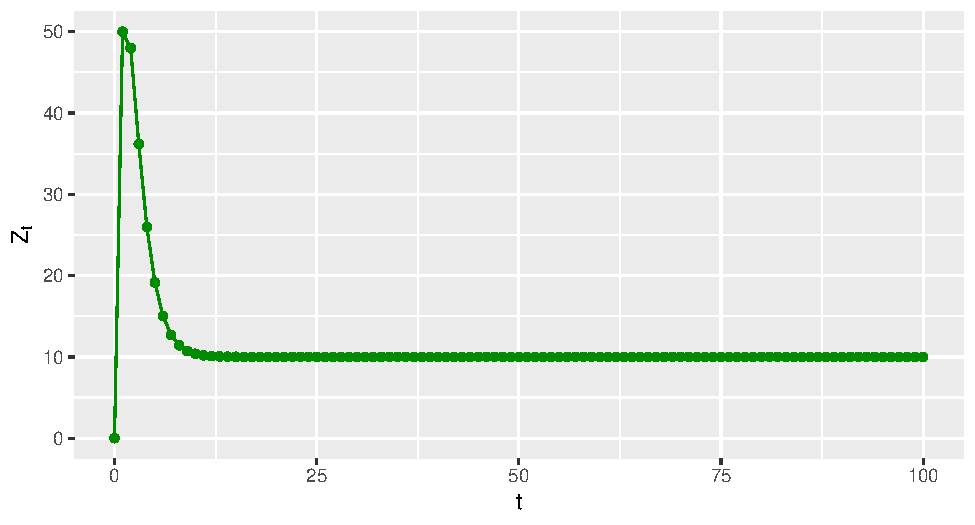
\includegraphics{Notas-Series-Tiempo_files/figure-latex/fig23-1} 

}

\caption{Evolución del proceso dado por $Z_t =3+0.9Z_{t-1}-0.2Z_{t-2}$}\label{fig:fig23}
\end{figure}

Por el Teorema Fundamental del Álgebra es posible escribir a la ecuación \eqref{eq:EDOP2} como:
\begin{eqnarray}
    (1 - g_1 L)(1 - g_1 L) \ldots (1 - g_p L) Z_t & = & a_0
    \label{eq:EDOP3}
\end{eqnarray}

Utilizando la ecuación \eqref{eq:EDOP2} y la ecuación \eqref{eq:EDOP3} tenemos que la solución general de una ecuación como la descrita en \eqref{eq:EDOP} se puede escribir como:
\begin{equation}
    Z_t  =  \frac{a_0}{1 - a_1 - a_2 - \ldots - a_p} + s_1 g^t_1 + s_2 g^t_2 + \ldots + s_p g^t_p \\
    \label{eq:EDOPGEN}
\end{equation}\\
\begin{eqnarray}
    Z_t & = & \frac{a_0}{(1 - g_1)(1 - g_1) \ldots (1 - g_p)} + s_1 g^t_1 + s_2 g^t_2 + \ldots + s_p g^t_p 
    \label{eq:EDOPGEN2}
\end{eqnarray}

Donde \(s_1\), \(s_2\), \ldots, \(s_p\) son cosntantes que se determinan utilizando \(p\) valores partículares de \(Z_t\), y la solución general descrita en las ecuaciones \eqref{eq:EDOPGEN} y \eqref{eq:EDOPGEN2} implica encontrar \(p\) raíces: \(x_1 = g^{-1}_1\), \(x_2 = g^{-1}_2\), \ldots, \(x_p = g^{-1}_p\) de los siguientes polinomios equivalentes:
\begin{eqnarray}
    (1 - g_1)(1 - g_1) \ldots (1 - g_p) = 0
    \label{eq:POLGEN1}
\end{eqnarray}

\begin{eqnarray}
    1 - a_1 x - a_2 x^2 - \ldots - a_p x^p = 0
    \label{eq:POLGEN2}
\end{eqnarray}

\begin{eqnarray}
    a_p x^p + \ldots + a_2 x^2 + a_1 x - 1 = 0
    \label{eq:POLGEN3}
\end{eqnarray}

Antes de plantear la solución general, analicemos una solución patícular cuando un conjunto de las \(p\) raíces, digamos un total de \(m\), son iguales, es decir, cuando sucede que \(g_1 = g_2 = \ldots = g_m = g\) (con \(1 < m \leq p\)). En este caso la solución general en la ecuación \eqref{eq:EDOPGEN2} se escribe como:
\begin{eqnarray}
    Z_t & = & \frac{a_0}{(1 - g)^m(1 - g_{m+1}) \ldots (1 - g_p)} \nonumber \\ 
    & & + s_1 g^t + s_2 t g^t + \ldots + s_m t^{m-1} g^t + s_{m+1} g^t_{m+1} + \ldots + s_{p} g^t_{p}
    \label{eq:EDOPGEN3}
\end{eqnarray}

Definamos:
\begin{equation}
    f(g) = \frac{1}{1 - g} = \sum_{j = 0}^{\infty} g^j
    \label{eq:EDOPGEN4}
\end{equation}

Si retomamos el método descrito parráfos arriba tenemos las siguientes expresiones. Cuando \(m = 2\):
\begin{equation}
    f'(g) = \frac{1}{(1 - g)^2} = \sum_{j = 0}^{\infty} j g^{j-1} = \sum_{j = 0}^{\infty} (1 + j) g^j \nonumber
\end{equation}

En el otro extremo, cuando \(m = p\):
\begin{equation}
    f^{(p-1)}(g) = \frac{p-1}{(1 - g)^p} = \sum_{j = 0}^{\infty} \frac{(p-1+j)(p-2+j) \ldots (2+j)(1+j)}{(p-1)!} g^j
    \label{eq:EDOPGEN5}
\end{equation}

Así, en el extremo cuando \(m = p\) la solución general podría estar dada por:
\begin{eqnarray}
    Z_t & = & a_0 \sum_{j = 0}^{\infty} \frac{(p-1+j)(p-2+j) \ldots (2+j)(1+j)}{(p-1)!} g^j \nonumber \\
    & & + g^t \sum_{i = 0}^p s_i t^{i-1}
    \label{eq:EDOPGEN6}
\end{eqnarray}

Donde \(|{g} < 1|\), \(t = \ldots, -2, -1, 0, 1, 2, \ldots\). Para finalizar esta sección, plantearemos la expresión de polinomio característico que nos permitirá hacer el análisis de convergencia de los procesos. Partamos de que la ecuación \eqref{eq:POLGEN3} se puede escribir como:
\begin{equation}
    (x^{-1})^p - a_1 (x^{-1})^{p-1} - a_2 (x^{-1})^{p-1} - \ldots - a_p = 0
    \label{eq:POLGEN55}
\end{equation}

La ecuación \eqref{eq:POLGEN55} permite interpretar las raíces del polinomio característico de forma directa ya que \(x^{-1}_1 = g_1\), \(x^{-1}_2 = g_2\), \ldots, \(x^{-1}_p = g_p\). Así, siempre que \(p \geq 1\) en la ecuación \eqref{eq:EDOP}, diremos que el proceso descrito en esa ecuación dará como resultado un proceso convergente si se cumplen las dos condiciones \eqref{eq:COND1} y \eqref{eq:COND2}:
\begin{equation}
    |a_p| < 1  
    \label{eq:COND1}
\end{equation}
\begin{equation}
    a_1 + a_2 + \ldots + a_p < 1
    \label{eq:COND2}
\end{equation}

Alternativamente, cuando las raíces son reales lo anterior es equivalente a la expresión \eqref{eq:COND3}:
\begin{eqnarray}
    |g_i| < 1
    \label{eq:COND3}
\end{eqnarray}

Para \(\forall i = 1, 2, \ldots, p\). Cuando la raíces son imaginarias, las dos condiciones \eqref{eq:COND1} y \eqref{eq:COND2} son equivalentes a la expresión \eqref{eq:COND4}:
\begin{eqnarray}
    \sqrt{g_i g_j} = \sqrt{u^2 + v^2} < 1 
    \label{eq:COND4}
\end{eqnarray}

Para \(\forall i \neq j\) y \(i, j = 1, 2, \ldots, p\). Cuando \(g_1 = g_2 = \ldots = g_p = g\), la condición de la ecuación \eqref{eq:COND3} se resume a que \(|g| < 1\). En resumen, las condiciones descritas en las ecuaciones \eqref{eq:COND3} y \eqref{eq:COND4} se puden ilustrar con un circulo unitario como el de la Figura \ref{fig:fig24} en que sí las raíces se ubican dentro de éste, podemos decir que el proceso es convergente en el largo plazo.

\begin{figure}

{\centering 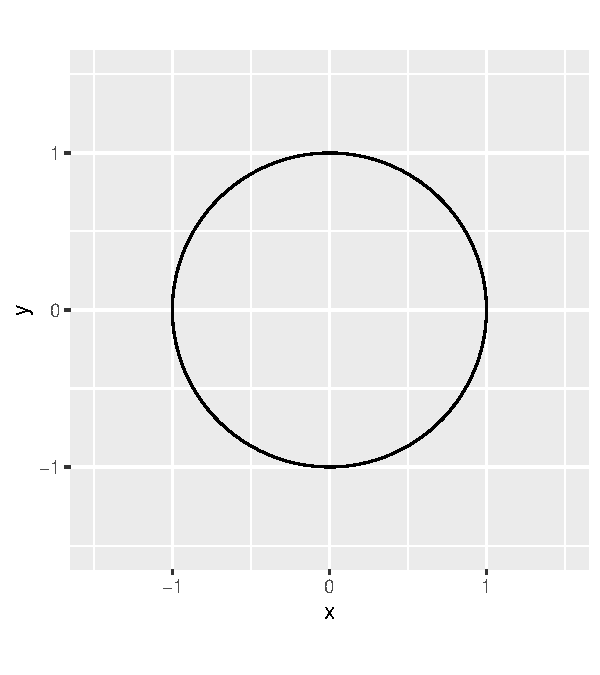
\includegraphics{Notas-Series-Tiempo_files/figure-latex/fig24-1} 

}

\caption{Circulo unitario en el que se cumple que $|g_i|<1$ y $(g_i g_j)^{1/2} = (u^2 + v^2)^{1/2} < 1$}\label{fig:fig24}
\end{figure}

\hypertarget{operador-de-rezago-l}{%
\section{Operador de rezago L}\label{operador-de-rezago-l}}

Denotemos, como se ha mencionado con anterioridad, con \(L\) al operador de rezago, el cual nos permitirá construir una relación entre diferencias y medias móviles como se verá más adelante en los procesos univariados \(AR(p)\), \(MA(q)\) y, en general, \(ARIMA(p, d, q)\). Sean \(X\), \(Y\) o \(Z\) variables con las que denotaremos a una serie de tiempo (note que hasta el momento no hemos definido qué es una serie de tiempo, no obstante no es necesario definirla para hacer uso del operador).

En esta sección resumiremos algunas propiedades usadas en el capítulo y en capítulos más adelante. Así, si a dicha serie le aplicamos el operador rezago antes definido, el resultado deberá ser que cada uno de los valores de la serie es retardado o regresado un período. Es decir:

\begin{equation}
    L Z_t = Z_{t-1}
    \label{eq:Lag1}
\end{equation}

De esta forma, si aplicamos el operador rezago \(L\) a la nueva serie de tiempo dada por \(Z_{t-1}\) podemos obtener \(Z_{t-2}\), haciendo uso de la ecuación \eqref{eq:Lag1} podemos obtener:
\begin{equation}
    L Z_{t-1} = L(L Z_t) = L^2 Z_t = Z_{t-2}
    \label{eq:Lag2}
\end{equation}

Mediante una generalización podemos obtener:
\begin{equation}
    L^k Z_t = Z_{t-k}
    \label{eq:Lag3}
\end{equation}

Para \(k = \ldots, -2, -1, 0, 1, 2, \ldots\). Así, para \(k = 0\) obtenemos la identidad dado que \(L^0 Z_t = Z_t\), de tal forma que siempre asumiremos que \(L^0 = 1\). En otro caso, cuando \(k > 0\) a la serie de tiempo a la cual se le aplique el operador rezago \(L\) se le deberá aplicar un rezago de \(k\) periodos a cada uno de los elementos de la serie. Por el contrario, cuando \(k < 0\) el operador rezago significa que se deberá adelantar \(|k|\) veces a cada elemento de la serie. Por ejemplo, \(L^{-3} Z_t = Z_{t+3}\).

Las reglas descritas en lo subsecuente se mantienen indistintamene cuando aplican para el caso de rezagar como para cuando se adelanta una serie. Como primera propiedad tomemos a la siguiente propiedad:
\begin{equation}
    L^{m} Z_{t-n} = L^{m} (L^{n} Z_{t}) = L^{m + n} Z_{t} = Z_{t-(n + m)} 
    \label{eq:Lag4}
\end{equation}

De lo anterior podemos inferir el siguiente resultado:
\begin{equation}
    \Delta Z_{t} = Z_{t} - Z_{t-1} = (1 - L) Z_{t} 
    \label{eq:Lag5}
\end{equation}

En el caso de la diferencia de órden cuatro o cuarta diferencia se puede expresar como:
\begin{equation}
    \Delta_{4} Z_{t} = Z_{t} - Z_{t-4} = (1 - L^4) Z_{t}
\label{eq:Diff4}
\end{equation}

Al respecto, vale la pena aclarar que en ocaciones se hará uso de una notación alternativa dada por: \(\Delta^k\) o \(\Delta_k\), donde \(k = 1, 2, 3, \ldots\), indistintamente, ya que en ambos casos se referirá a una diferencia de orden \(k\). Esta notación resulta de gran utilidad cuando se quiere comparar periodos equivalentes como, por ejemplo, el mismo trimestre pero de un año anterior. De forma similar, para el caso de logarítmos podemos escribir a la ecuación \eqref{eq:Diff4} como:
\begin{equation}
    \Delta^{4} ln(Z_{t}) = \Delta_{4} ln(Z_{t}) = ln(Z_{t}) - ln(Z_{t-4}) = (1 - L^4) ln(Z_{t}) 
    \label{eq:Diff5}
\end{equation}

Para el caso de una serie de tiempo que se le ha transformado mediante medias móviles, digamos de \(4\) periodos, podemos escribirla como:
\begin{equation}
    Zs_{t} = \frac{1}{4}(Z_{t} + Z_{t-1} + Z_{t-2} + Z_{t-3}) = \frac{1}{4}(1 + L + L^2 + L^3)Z_{t}
    \label{eq:Diff6}
\end{equation}

Una generalización del anterior caso puede ser escrito como un polinomio de orden \(p\) con el operador rezago \(L\) dado como:
\begin{eqnarray}
    \alpha(L) Z_{t} & = & (1 - \alpha_1 L - \alpha_2 L^2 - \ldots - \alpha_p L^p) Z_{t} \nonumber \\
    & = & Z_{t} - \alpha_1 Z_{t-1} - \alpha_2 Z_{t-2} - \ldots - \alpha_p Z_{t-p}
\label{eq:Ecp1}
\end{eqnarray}

Donde \(\alpha_i\) puede ser remplazada por cualquier constante \(a_i\), con \(i = 1, 2, 3, \ldots\), para escribir ecuaciones como las anteriores. Adicionalmente, podemos decir que la ecuación \eqref{eq:Ecp1} es una generalización del caso de medias móviles, el cual admite una poderación distinta para cada uno de los elementos rezagados.

Existe la posibilidad de operar más de un polinomio a la vez. Para múltiples polinomios (digamos, los polinomios \(\alpha(L)\) y \(\beta(L)\)) podemos escribir el siguiente resultado:
\begin{equation}
    \alpha(L) \beta(L) = \beta(L) \alpha(L)
    \label{eq:Diff7}
\end{equation}

Tales polinomios del operador rezago también son llamados \emph{filtros lineales}. A manera de ejemplo tomemos el siguiente caso de diferencias para una serie de \(Z_t\):
\begin{equation}
    \Delta Z_{t} = (1 - L) Z_{t} = Z_{t} - Z_{t-1} 
    \label{eq:Diff8}
\end{equation}

y un proceso de medias móviles para la misma serie de \(Z_t\):
\begin{equation}
    Zs_{t} = \frac{1}{4}(1 + L^1 + L^2 + L^3) Z_{t} = \frac{1}{4}(Z_{t} + Z_{t-1} + Z_{t-2} + Z_{t-3}) 
    \label{eq:Diff9}
\end{equation}

De tal forma que el producto de ambos procesos se puede escribir como:
\begin{equation}
(1 - L) \times \frac{1}{4}(1 + L^1 + L^2 + L^3) Z_{t} = \frac{1}{4}(1 - L^4) Z_{t}
\label{eq:Diff10}
\end{equation}

Es decir, que el producto de dos polinomios, uno de diferencias y otro más de medias móviles, resulta en uno de diferencias pero de mayor grado, en este caso de grado 4.

\hypertarget{modelos-de-series-de-tiempo-estacionarias}{%
\chapter{Modelos de Series de Tiempo Estacionarias}\label{modelos-de-series-de-tiempo-estacionarias}}

\hypertarget{definiciuxf3n-de-ergodicidad-y-estacionariedad}{%
\section{Definición de ergodicidad y estacionariedad}\label{definiciuxf3n-de-ergodicidad-y-estacionariedad}}

A partir de esta sección introduciremos mayor formalidad matemática al análisis de las series de tiempo. Por ello cambiaremos un poco la notación y ocuparemos a \(X_t\) en lugar de \(Z_t\) como objeto de nuestro análisis. Con \(X_t\) denotaremos a una serie de tiempo, ya que con \(Z_t\) denotareemos a una variable, sin que ella fuera necesariamente una serie de tiempo en los términos que a continuación discutimos. Asimismo, iniciaremos por establecer una serie de definiciones.

De esta forma, definiremos a una \emph{serie de tiempo} como un vector de variables aleatorias de dimensión \(T\), dado como:
\begin{equation}
    X_1, X_2, X_3, \ldots ,X_T
    \label{eq:Serie0}
\end{equation}

Cada una de las \(X_t\) (\(t = 1, 2, \ldots, T\)) consideradas como una variable aleatoria. Así, también podemos denotar a la serie de tiempo como:
\begin{equation}
    \{ X_t \}^T_{t = 1}
    \label{eq:Serie}
\end{equation}

Es decir, definiremos a \emph{una serie de tiempo como una realización de un proceso estocástico} --o un Proceso Generador de Datos (PGD). Consideremos una muestra de los múlples posibles resultados de muestras de tamaño \(T\), la colección dada por:
\begin{equation}
    \{X^{(1)}_1, X^{(1)}_2, \ldots, X^{(1)}_T\}
    \label{eq:Serie1}
\end{equation}

Digamos que la ecuación \eqref{eq:Serie1} es una de las tantas posibles resultantes del proceso estocástico o PGD. Eventualmente podríamos estar dispuestos a observar este proceso indefinidamente, de forma tal que estemos interesados en observar a la secuencia dada por \(\{ X^{(1)}_t \}^{\infty}_{t = 1}\), lo cual no dejaría se ser sólo una de las tantas realizaciones o secuencias del proceso estocástico original.

Tan solo por poner un ejemplo, podríamos observar las siguientes realizaciones del mismo PGD:
\begin{eqnarray*}
    & \{X^{(2)}_1, X^{(2)}_2, \ldots, X^{(2)}_T\} & \\
    & \{X^{(3)}_1, X^{(3)}_2, \ldots, X^{(3)}_T\} & \\
    & \{X^{(4)}_1, X^{(4)}_2, \ldots, X^{(4)}_T\} & \\
    & \vdots & \\
    & \{X^{(j)}_1, X^{(j)}_2, \ldots, X^{(j)}_T\} & 
\end{eqnarray*}

Donde \(j \in \mathbb{Z}\). En lo subsecuente, diremos que una serie de tiempo es una realización del proceso estocástico subyacente. Considerando, en consecuencia, al proceso estocástico con todas sus posibilidades de realización.

Para hacer más sencilla la notación no distinguiremos entre el proceso en sí mismo y una de sus realizaciones, es decir, siempre escribiremos a una serie de tiempo como la secuencia mostrada en la ecuación \eqref{eq:Serie}, o más precisamente como la siguiente realización:
\begin{equation}
    \{ X_1, X_2, \ldots, X_T \}
    \label{eq:Serie2}
\end{equation}

O simplemente:
\begin{equation}
    X_1, X_2, \ldots, X_T
    \label{eq:Serie3}
\end{equation}

El proceso estocástico de dimensión \(T\) puede ser completamente descrito por su función de distribución multivaraida de dimensión \(T\). No obstante, esto no resulta ser práctico cuando se opere más adelante en el curso. Por ello, en el curso, y en general casi todos los textos lo hacen, sólo nos enfocaremos en sus primer y segundo momentos, es decir, en sus medias o valores esperados:
\begin{equation*}
    \mathbb{E}[X_t]
\end{equation*}

Para \(t = 1, 2, \ldots, T\); o:
\begin{equation*}
\left[
    \begin{array}{c}
    \mathbb{E}[X_1] \\
    \mathbb{E}[X_2] \\
    \vdots \\
    \mathbb{E}[X_T]
    \end{array}
\right]
\end{equation*}

o,
\begin{equation*}
\left[
    \begin{array}{c}
    \mathbb{E}[X_1], \mathbb{E}[X_2], \ldots, \mathbb{E}[X_T]
    \end{array}
\right]
\end{equation*}

De sus variazas:
\begin{equation*}
    Var[X_t] = \mathbb{E}[(X_t - \mathbb{E}[X_t])^2]
\end{equation*}

Para \(t = 1, 2, \ldots, T\), y de sus \(T(T-1)/2\) covarianzas:
\begin{equation*}
    Cov[X_t,X_s] = \mathbb{E}[(X_t - \mathbb{E}[X_t])(X_s - \mathbb{E}[X_s])]
\end{equation*}

Para \(t < s\). Por lo tanto, en la forma matricial podemos escribir lo siguiente:
\begin{equation*}
\left[
    \begin{array}{c c c c}
    Var[X_1] & Cov[X_1,X_2] & \cdots & Cov[X_1,X_T] \\
    Cov[X_2,X_1] & Var[X_2] & \cdots & Cov[X_2,X_T] \\
    \vdots & \vdots & \ddots & \vdots \\
    Cov[X_T,X_1] & Cov[X_T,X_2] & \cdots & Var[X_T] \\
    \end{array}
\right]
\end{equation*}

\begin{equation}
= \left[
    \begin{array}{c c c c}
    \sigma_1^2 & \rho_{12} & \cdots & \rho_{1T} \\
    \rho_{21} & \sigma_2^2 & \cdots & \rho_{2T} \\
    \vdots & \vdots & \ddots & \vdots \\
    \rho_{T1} & \rho_{T2} & \cdots & \sigma_T^2 \\
    \end{array}
\right]
    \label{eq:MATCOV}
\end{equation}

Donde es claro que en la matriz de la ecuación \eqref{eq:MATCOV} existen \(T(T-1)/2\) covarianzas distintas, ya que se cumple que \(Cov[X_t,X_s] = Cov[X_s,X_t]\), para \(t \neq s\).

A menudo, esas covarianzas son denominadas como autocovarianzas puesto que ellas son covarianzas entre variables aleatorias pertenecientes al mismo proceso estocástico pero en un momento \(t\) diferente. Si el proceso estocástico tiene una distribución normal multivariada, su función de distribución estará totalmente descrita por sus momentos de primer y segundo orden.

Ahora introduciremos el concepto de ergodicidad, el cual indica que los momentos muestrales, los cuales son calculados en la base de una serie de tiempo con un número finito de observaciones, en la medida que \(T \rightarrow \infty\) sus correspondientes momentos muestrales, tienden a los verdaderos valores poblacionales, los cuales definiremos como \(\mu\), para la media, y \(\sigma^2_X\) para la varianza.

Este concepto sólo es cierto si asumimos que, por ejemplo, el valor esperado y la varianza son como se dice a continuación para todo \(t = 1, 2, \ldots, T\):
\begin{eqnarray}
    \mathbb{E}[X_t] = \mu_t = \mu \\
    \label{MEDIA}
    \label{eq:ESPERANZA}
\end{eqnarray}
\begin{eqnarray}
    Var[X_t] = \sigma^2_X
    \label{eq:VARIANZA}
\end{eqnarray}

Mas formalmente, se dice que el PGD o el proceso estocástico es ergódico en la media si:
\begin{equation}
    \displaystyle\lim_{T \to \infty}{\mathbb{E} \left[ \left( \frac{1}{T} \sum^{T}_{t = 1} (X_t - \mu) \right) ^2 \right]} = 0
    \label{eq:LIM1}
\end{equation}

y ergódico en la varianza si:
\begin{equation}
    \displaystyle\lim_{T \to \infty}{\mathbb{E} \left[ \left( \frac{1}{T} \sum^{T}_{t = 1} (X_t - \mu) ^2 - \sigma^2_X \right) ^2 \right]} = 0
    \label{eq:LIM2}
\end{equation}

Estas condiciones se les conoce como \emph{propiedades de consistencia} para las variables aleatorias. Sin embargo, éstas no pueden ser probadas. Por ello se les denomina como un supuesto que pueden cumplir algunas de las series. Más importante aún: \textbf{un proceso estocástico que tiende a estar en equilibrio estadístico en un orden ergódico, es estacionario}.

Podemos distinguir dos tipos de estacionariedad. Si asumimos que la función común de distribución del proceso estocástico no cambia a lo largo del tiempo, se dice que el proceso es \emph{estrictamente estacionario}. Como este concepto es dificil de aplicar en la práctica, solo consideraremos a la \emph{estacionariedad débil} o estacionariedad en sus momentos.

Definiremos a la estacionariedad por sus momentos del correspondiente proceso estocástico dado por \(\{X_t\}\):

\begin{enumerate}
\def\labelenumi{\arabic{enumi}.}
\item
  \emph{Estacionariedad en media}: Un proceso estocástico es estacionario en media si \(E[X_t] = \mu_t = \mu\) es constante para todo \(t\).
\item
  \emph{Estacionariedad en varianza}: Un proceso estocástico es estacionario en varianza si \(Var[X_t] = \mathbb{E}[(X_t - \mu_t)^2] = \sigma^2_X = \gamma(0)\) es constante y finita para todo \(t\).
\item
  \emph{Estacionariedad en covarianza}: Un proceso estocástico es estacionario en covarianza si \(Cov[X_t,X_s] = \mathbb{E}[(X_t - \mu_t)(X_s - \mu_s)] = \gamma(|s-t|)\) es sólo una función del tiempo y de la distancia entre las dos variables aleatorias. Por lo que no depende del tiempo denotado por \(t\) (no depende de la información contemporánea).
\item
  \emph{Estacionariedad débil}: Como la estacionariedad en varianza resulta de forma inmediata de la estacionariedad en covarianza cuando se asume que \(s = t\), un proceso estocástico es débilmente estacionario cuando es estacionario en media y covarianza.
\end{enumerate}

Puesto que resulta poco factible asumir una estacionariedad diferente a la débil, es adelante siempre que digamos que un proceso es estacionario se referirá al caso débil y sólo diremos que el proceso es estacionario, sin el apelativo de débil.

Ahora veamos un ejemplo de lo anterior. Supongamos una serie de tiempo denotada por: \(\{U_t\}^T_{t = 0}\). Decimos que el proceso estocástico \(\{U_t\}\) es un \emph{proceso estocástico puramente aleatorio} o es un \emph{proceso estocástico de ruido blanco o caminata aleatoria}, si éste tiene las siguientes propiedades:
1. \(\mathbb{E}[U_t] = 0\), \(\forall t\);
2. \(Var[U_t] = \mathbb{E}[(U_t - \mu_t)^2] = \mathbb{E}[(U_t - \mu)^2] = \mathbb{E}[(U_t)^2] = \sigma^2\), \(\forall t\), y
3. \(Cov[U_t,U_s] = \mathbb{E}[(U_t - \mu_t)(U_s - \mu_s)] = \mathbb{E}[(U_t - \mu)(U_s - \mu)] = \mathbb{E}[U_t U_s] = 0\), \(\forall t \neq s\).

En otras palabras, un proceso \(U_t\) es un ruido blanco si su valor esperado (promedio) es cero (0), tiene una varianza finita y constante, y además no le importa la historia pasada. Así, su valor presente no se ve influenciado por sus valores pasados no importando respecto de que periodo se tome referencia.

En apariencia, por sus propiedades, este proceso es débilmente estacionario --o simplemente, estacionario--. Todas las variables aleatorias tienen una media de cero, una varianza \(\sigma^2\) y no existe correlación entre ellas.

Propongamos un ejemplo para ilustrar la teoría previa. Supongamos que definimos un nuevo proceso estocástico \(\{X_t\}\) como:
\begin{equation}
    X_t = \left\{ \begin{array}{l} U_0  \mbox{ para } t = 0 \\ X_{t-1} + U_t \mbox{ para } t = 1, 2, 3, \ldots \end{array}\right.
    \label{eq:em1}
\end{equation}

Donde \(\{ U_t \}\) es un proceso puramente aleatorio. Este proceso estocástico, o caminata aleatoria sin tendencia (ajuste - drift), puede ser reescrito como:
\begin{equation}
    X_t = \sum^t_{j = 0} U_j
    \label{eq:em2}
\end{equation}

Tratemos de dar más claridad al ejemplo, para ello asumamos que generamos a \(\{U_t\}\) por medio del lanzamiento de una moneda. Donde obtenemos una cara (águila) con una probabilidad de \(0.5\), en cuyo caso decimos que la variable aleatoria \(U_t\) tomará el valor de \(+1\), y una cruz (sol) con una probabilidad de \(0.5\), en cuyo caso decimos que la variable aleatoria \(U_t\) toma el valor de \(-1\).

Este planteamiento cumple con las propiedas enunciadas ya que:
1. \(\mathbb{E}[U_t] = 0.5 \times -1 + 0.5 \times 1 = 0\), \(\forall t\)
2. \(Var[U_t] = \mathbb{E}[(U_t - 0)^2] = \frac{1}{2}((-1)^2) + \frac{1}{2}((1)^2) = 1\), \(\forall t\)
3. \(Cov[U_t,U_s] = \mathbb{E}[(U_t - 0)(U_s - 0)] = \mathbb{E}[U_t \cdot U_s] = 0\), \(\forall t \neq s\).

Retomando a nuestro proceso \(X_t\), diremos que el caso de \(X_0 = 0\), para \(t = 0\). Si verificamos cúales son sus primeros y segundos momentos de \(\{X_t\}\) tenemos:
\begin{equation}
    \mathbb{E}[X_t] = \mathbb{E}\left[ \sum^t_{j=1} U_j \right] = \sum^t_{j=1} \mathbb{E}[U_j] = 0
    \label{eq:em3}
\end{equation}

En cuanto a la varianza:
\begin{eqnarray}
    Var[X_t] & = & Var \left[ \sum^t_{j=1} U_j \right] \nonumber \\
    & = & \sum^t_{j=1} Var[U_j] + 2 * \sum_{j \neq k} Cov[U_j,U_k] \nonumber \\
    & = & \sum^t_{j=1} 1 \nonumber \\
    & = & t
    \label{eq:em4}
\end{eqnarray}

Lo anterior, dado que hemos supuesto que en la caminata aleatoria todas la variables aleatorias son independientes, es decir, \(Cov[U_t,U_s] = E[U_t \cdot U_s] = 0\). Por su parte, la covarianza del proceso estocástico se puede ver como:
\begin{eqnarray*}
    Cov[X_t,X_s] & = & \mathbb{E} \left[ \left( \sum^t_{j=1} U_j - 0 \right) \left( \sum^s_{i=1} U_i - 0 \right) \right] \\
    & = & \mathbb{E}[(U_1 + U_2 + \ldots + U_t)(U_1 + U_2 + \ldots + U_s)] \\
    & = & \sum^t_{j=1} \sum^s_{i=1} \mathbb{E}[U_j U_i] \\
    & = & \mathbb{E}[U^2_1] + \mathbb{E}[U^2_2] + \ldots + \mathbb{E}[U^2_k] \\
    & = & \sigma^2 + \sigma^2 + \ldots + \sigma^2 \\
    & = & 1 + 1 + 1 + 1 \\
    & = & min(t,s)
\end{eqnarray*}

\textbackslash begin\{figure\}

\{\centering 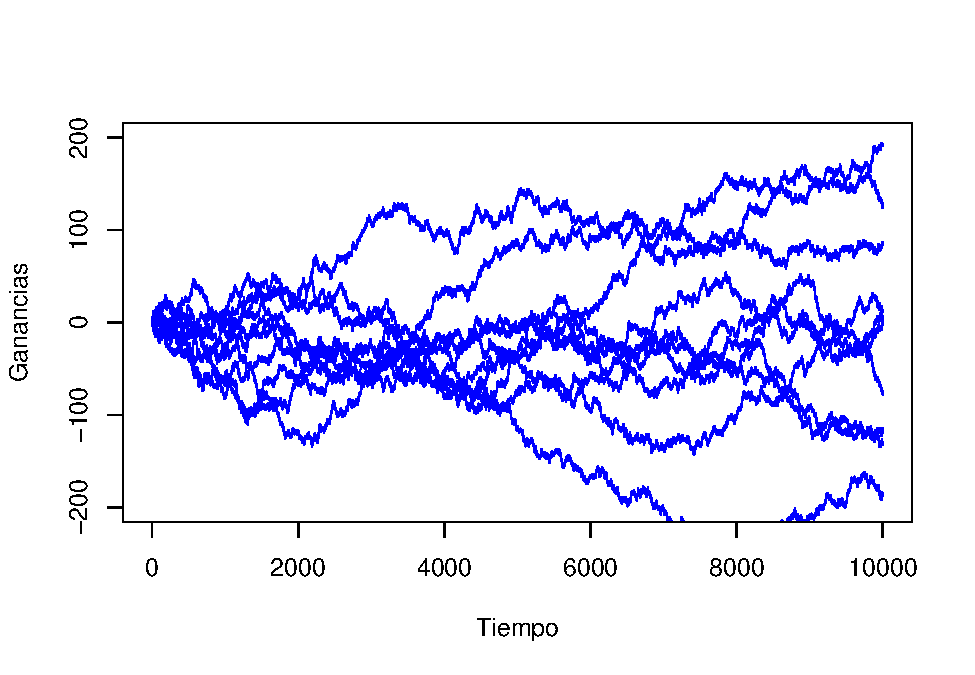
\includegraphics{Notas-Series-Tiempo_files/figure-latex/fig31-1}

\}

\textbackslash caption\{Ejemplo de 10 trayectorias de la caminata aleatoria, cuando sólo es posible cambios de +1 y -1\$\}\label{fig:fig31}
\textbackslash end\{figure\}

Así, el proceso estocástico dado por la caminata alaeatoria sin un término de ajuste es estacionario en media, pero no en varianza o en covarianza, y consecuentemente, en general no estacionario, condición que contraria al caso del proceso simple descrito en \(U_t\).

Es facil ver que muchas de las posibilidades de realización de este proceso estocástico (series de tiempo) pueden tomar cualquiera de las rutas consideradas en el Figura \ref{fig:fig31}.

\hypertarget{funciuxf3n-de-autocorrelaciuxf3n}{%
\section{Función de autocorrelación}\label{funciuxf3n-de-autocorrelaciuxf3n}}

Para ampliar la discusión, es posible calcular la fuerza o intensidad de la dependencia de las variables aleatorias dentro de un proceso estocástico, ello mediante el uso de las autocovarianzas. Cuando las covarianzas son normalizadas respecto de la varianza, el resultado es un término que es independiente de las unidad de medida aplicada, y se conoce como la \emph{función de autocorrelación}.

Para procesos estacionarios, dicha función de autocorrelación esta dada por:
\begin{equation}
    \rho(\tau) = \frac{\mathbb{E}[(X_t - \mu)(X_{t+\tau} - \mu)]}{\mathbb{E}[(X_t - \mu)^2]} = \frac{\gamma(\tau)}{\gamma(0)}
    \label{eq:em5}
\end{equation}

Donde \(\tau = \ldots, -2, -1, 0, 1, 2, \ldots\). Dicha función tiene las siguientes propiedades:

\begin{enumerate}
\def\labelenumi{\arabic{enumi}.}
\tightlist
\item
  \(\rho(0) = 1\). Es fácil demostrar que la función \(\rho(0)\) es:
\end{enumerate}

\begin{equation}
    \rho(0) = \frac{\mathbb{E}[(X_t - \mu)(X_{t + 0} - \mu)]}{\mathbb{E}[(X_t - \mu)^2]} = \frac{\mathbb{E}[(X_t - \mu)^2]}{\mathbb{E}[(X_t - \mu)^2]} = 1
\end{equation}

\begin{enumerate}
\def\labelenumi{\arabic{enumi}.}
\setcounter{enumi}{1}
\tightlist
\item
  \(\rho(\tau) = \rho(-\tau)\). Partiendo de la definción de \(\rho(\tau)\) podemos ver que la distancia que existe entre \(t\) y \(t + \tau\) es \(\tau\), de esta forma la autocorrelación de la variable \(X\) entre los periodos antes señalados debería ser la misma para el caso en que \(\rho(-\tau)\). Partamos de la ecuación para ver más claramente:
\end{enumerate}

\begin{equation}
    \rho(\tau) = \frac{\mathbb{E}[(X_t - \mu)(X_{t + \tau} - \mu)]}{\mathbb{E}[(X_t - \mu)^2]} = \frac{\mathbb{E}[(X_t - \mu)(X_{t - \tau} - \mu)]}{\mathbb{E}[(X_t - \mu)^2]} = \rho(-\tau)
\end{equation}

\begin{enumerate}
\def\labelenumi{\arabic{enumi}.}
\setcounter{enumi}{2}
\tightlist
\item
  \(\lvert\rho(\tau)\lvert \leq 1\), para todo \(\tau\).
\end{enumerate}

Derivado de las propiedades 1 y 2 antes descritas se puede concluir que sólo es necesario conocer la función de autocorrelación para el caso de \(\tau = 1, 2, 3, \ldots\), ya que de estos casos podemos derivar los valores de la función de autocorrelación complementarios de \(\tau = \ldots, -3, -2, -1\).

Partiendo de los supuestos de ergodicidad en relación a la media, varianza y covarianzas de un proceso estacionario, podemos estimar dichos paramétros con las siguientes formulaciones o propuestas de estimadores puntuales:
\begin{equation}
    \hat{\mu} = \frac{1}{T} \sum^T_{t=1} X_t
    \label{eq:em6}
\end{equation}

\begin{equation}
    \hat{\gamma}(0) = \frac{1}{T} \sum^T_{t=1} (X_t - \hat{\mu})^2 = \hat{\sigma}^2
    \label{eq:em7}
\end{equation}

\begin{equation}
    \hat{\gamma}(\tau) = \frac{1}{T} \sum^{T - \tau}_{t=1} (X_t - \hat{\mu})(X_{t+\tau} - \hat{\mu}) \mbox{, para } \tau = 1, 2, \ldots, T-1
    \label{eq:em8}
\end{equation}

No hacemos la demostración en estas notas --sería deseable que el alumno revisará la afimación-- pero estos últimos son estimadores consistentes de \(\mu\), \(\gamma(0)\) y \(\gamma(\tau)\). Por su parte, un estimador consistente de la función de autocorrelación estará dado por:
\begin{equation}
\hat{\rho}(\tau) = \frac{\sum^{T - \tau}_{t=1} (X_t - \hat{\mu})(X_{t+\tau} - \hat{\mu})}{\sum^T_{t=1} (X_t - \hat{\mu})^2} = \frac{\hat{\gamma}(\tau)}{\hat{\gamma}(0)}
\label{eq:eqautocorr}
\end{equation}

El estimador de la ecuación \eqref{eq:eqautocorr} es asintóticamente insesgado. Por ejemplo, para el caso de un proceso de ruido blanco o caminata aleatoria, su varianza puede ser aproximada por el valor dado \(1/T\). Ésta tiene, asintóticamente, una distribución normal. Dado esto, el intervalo de confianza al \(95\%\) será el dado por \(\pm 2/\sqrt{T}\), en el cual se encuentra la mayoría de los coeficientes de autocorrelación estimados.

Ahora discutamos algunos ejemplos o aplicaciones. Cuando se realiza la evaluación de la estimación de un modelo de series de tiempo es importante saber si los residuales del modelo realmente tienen propiedades de un proceso puramente aleatorio, en partícular, si ellos no están correlacionados entre sí. Así, la hipotésis a probar será:
\begin{equation}
    H_0 : \rho(\tau) = 0 \mbox{, para todo } \tau = 1, 2, \ldots, m \mbox{ y } m < T
    \label{eq:eqautocorr1}
\end{equation}

Esta expresión se puede interpretar como una prueba respecto de si la correlación entre la información de periodos atrás es cero con la información contemporánea. Para hacer una pruena global de la hipotésis de sí un número \(m\) de coeficientes de autocovarianzas son cero Box y Pierce (1970) desarrollarón la siguiente estadística:
\begin{equation}
    Q^* = T \sum_{j = 1}^{m} \hat{\rho} (j)^2
    \label{eq:eqautocorr2}
\end{equation}

Bajo la hipotésis nula esta estadística se distribulle asintóticamente como una chi cuadrado (\(\chi^2\)) con \(m-k\) grados de libertad y con \(k\) que representa al número de paramétros estimados.

Haciendo una aplicación estricta de la distribución de esta estadística, sabemos que esta se mantiene asintóticamente. Greta, Ljung y Box (1978) propusieron la siguiente modificación de la estadística para muestras pequeñas:
\begin{equation}
    Q = T(T + 2) \sum_{j = 1}^{m} \frac{\hat{\rho} (j)^2}{T - j}
    \label{eq:eqautocorr3}
\end{equation}

La cual también se distribulle asintóticamente como \(\chi^2\) con \(m-k\) grados de libertad.

También es intuitivamente claro que la hipótesis nula de no autocorrelación de residuales debería ser rechazada si alguno de los valores \(\hat{\rho} (j)\) es muy grande, es decir, si \(Q\) o \(Q^*\) es muy grande. O más precisamente, si estas estadísticas son más grandes que los correspondientes valores críticos de la distribución \(\chi^2\) con \(m-k\) grados de libertad a algún grado dado de signficancia.

Una alternativa para esta prueba es una del tipo Multiplicadores de Lagrange (o LM) desarrollada por Breusch (1978) y Godfrey (1978). La cual, al igual que las estadísticas \(Q\) y \(Q^*\), la hipotesis nula está dada por:

\begin{quote}
\(H_0\): Los residuales no están autocorrelacionados.
\end{quote}

\begin{quote}
\(H_a\): Los residuales muestran alguna acutocorrelación de forma autoregresiva o de medias móviles.
\end{quote}

La prueba consiste en realizar una regresión auxiliar en la cual los residuales se estiman en función de las variables explicativas del modelo original y en los residuales mismos pero rezagados hasta el término \(m\) (regresión auxiliar). La prueba resulta en una estadìstica con una distribución \(\chi^2\) con \(m\) grados de libertad la cual está dada por la expresión:
\begin{equation}
    LM = T \times R^2
    \label{eq:eqautocorr4}
\end{equation}

Donde \(R^2\) es el resultante de la regresión auxiliar y \(T\) es el número de observaciones totales.

En comparación con una prueba Durbin - Watson que es comúnmente usada en la econometría tradicional, para probar autocorrelación de los residuales, las estadísticas \(Q\), \(Q^*\) y \(LM\) tienen las siguientes ventajas:

\begin{enumerate}
\def\labelenumi{\arabic{enumi}.}
\tightlist
\item
  Permiten corroborar la existencia de autocorrelación para cualquier orden, y no solo para un primer orden (es decir, para cualquier valor de \(\tau = 1, 2, 3, \ldots\));
\item
  Los resultados se mantienen aún y cuando exista una probable variable endógena en forma rezagada, y
\item
  No depende del orden o la forma en que se acomoden las observaciones, algo que es muy probalble que ocurra en la econometría tradicional.
\end{enumerate}

El hecho de los residuales no estén autocorrelacionados no implica que estos sean independientes y normalmente distribuidos. La ausencia de autocorrelación no implica una independencia estocástica si las variables son normalmente distribuidas.

A menudo se asume que estos residuales están distribuidos normalmente, ya que la mayoría de las pruebas estadísticas tienen este supuesto detrás. No obstante, ello también depende de los otros momentos de la distribución, específicamente del tercer y cuarto momento. Los cuales expresan como:
\begin{equation*}
    \mathbb{E}[(X_t - \mathbb{E}[X_t])^i] \mbox{, } i = 3, 4
\end{equation*}

El tercer momento es necesario para determinar el sesgo, el cual esta dado como:
\begin{equation}
    \hat{S} = \frac{1}{T} \frac{\sum_{t = 1}^{T} (X_t - \hat{\mu})^3}{\sqrt{\hat{\gamma}(0)^3}}
    \label{eq:eqautocorr6}
\end{equation}

Para distribuciones simetricas (como en el caso de la distribución normal) el valor teórico para el sesgo es cero.

La curtosis, la cual esta dada en función del cuarto momento, se puede expresar como:
\begin{equation}
    \hat{K} = \frac{1}{T} \frac{\sum_{t = 1}^{T} (X_t - \hat{\mu})^4}{\hat{\gamma}(0)^2}
    \label{eq:eqautocorr7}
\end{equation}

Para el caso de una distribución normal, esta estadística toma el valor de 3. Valores más grandes que 3 indican que la distribución tienen colas anchas. En tales casos se ubican a los datos financieros.

Usando el valor de las estadísticas para medir el sesgo y la curtosis, \(S\) y \(K\), respectivamente, Jarque y Bera (1980) propusieron una prueba de normalidad, la cual puede ser aplicada a series de tiempo en niveles o en diferencias indistintamente. Dicha prueba se expresa como:
\begin{equation}
    JB = \frac{T}{6} \left(\hat{S} + \frac{1}{4} (\hat{K} - 3)^2 \right) 
    \label{eq:eqautocorr8}
\end{equation}

La cual tiene una distribución \(\chi^2\) con \(2\) grados de libertad y donde \(T\) es el tamaño de la muestra. La hipótesis de que las observaciones están distribuidas de forma normal se rechaza si los valores de la estadística de prueba es más grande que los correspondientes valores criticos en tablas.

Veamos un ejemplo para ilustrar el uso de la función de autocorrelación. Tomemos como variable al número de pasajeros transportados por el sistema de transporte del metro de la CDMX.\footnote{Los datos y algoritmo está disponible en el repositorio de GitHub y corresponde a la Clase 3.} Los datos empleados fueron tomados del INEGI y son una serie de tiempo en el periodo que va de enero de 2000 a junio de 2019, es decir, 234 observaciones. Como se puede apreciar en la Figura \ref{fig:fig32}, el número de pasajeros por mes ha oscilado significativamente a lo largo de tiempo. Incluso podemos observar un cambio estructural de la serie entre 2011 y 2012. Asimismo, podemos ubicar una caida atípica que ocurrió en septiembre de 2017.

\begin{Shaded}
\begin{Highlighting}[]
\FunctionTok{library}\NormalTok{(ggplot2)}
\FunctionTok{library}\NormalTok{(dplyr)}
\FunctionTok{library}\NormalTok{(readxl)}

\NormalTok{Datos }\OtherTok{\textless{}{-}} \FunctionTok{read\_excel}\NormalTok{(}\StringTok{"BD/Base\_Transporte.xlsx"}\NormalTok{, }\AttributeTok{sheet =} \StringTok{"Datos"}\NormalTok{, }\AttributeTok{col\_names =} \ConstantTok{TRUE}\NormalTok{)}

\FunctionTok{ggplot}\NormalTok{(}\AttributeTok{data =}\NormalTok{ Datos, }\FunctionTok{aes}\NormalTok{(}\AttributeTok{x =}\NormalTok{ Periodo, }\AttributeTok{y =}\NormalTok{ Pax\_Metro)) }\SpecialCharTok{+} 
  \FunctionTok{geom\_line}\NormalTok{(}\AttributeTok{linewidth =} \FloatTok{0.5}\NormalTok{, }\AttributeTok{color =} \StringTok{"darkblue"}\NormalTok{) }\SpecialCharTok{+}
  \CommentTok{\#geom\_point(size = 1.0, color = "darkblue") + }
  \CommentTok{\#theme\_bw() + }
  \FunctionTok{xlab}\NormalTok{(}\StringTok{"Tiempo"}\NormalTok{) }\SpecialCharTok{+} 
  \FunctionTok{ylab}\NormalTok{(}\StringTok{"Millones de pasajeros"}\NormalTok{) }\SpecialCharTok{+} 
  \FunctionTok{theme}\NormalTok{(}\AttributeTok{plot.title =} \FunctionTok{element\_text}\NormalTok{(}\AttributeTok{size =} \DecValTok{11}\NormalTok{, }\AttributeTok{face =} \StringTok{"bold"}\NormalTok{, }\AttributeTok{hjust =} \DecValTok{0}\NormalTok{)) }\SpecialCharTok{+} 
  \FunctionTok{theme}\NormalTok{(}\AttributeTok{plot.subtitle =} \FunctionTok{element\_text}\NormalTok{(}\AttributeTok{size =} \DecValTok{10}\NormalTok{, }\AttributeTok{hjust =} \DecValTok{0}\NormalTok{)) }\SpecialCharTok{+} 
  \FunctionTok{theme}\NormalTok{(}\AttributeTok{plot.caption =} \FunctionTok{element\_text}\NormalTok{(}\AttributeTok{size =} \DecValTok{10}\NormalTok{, }\AttributeTok{hjust =} \DecValTok{0}\NormalTok{)) }\SpecialCharTok{+}
  \FunctionTok{theme}\NormalTok{(}\AttributeTok{plot.margin =} \FunctionTok{unit}\NormalTok{(}\FunctionTok{c}\NormalTok{(}\DecValTok{1}\NormalTok{,}\DecValTok{1}\NormalTok{,}\DecValTok{1}\NormalTok{,}\DecValTok{1}\NormalTok{), }\StringTok{"cm"}\NormalTok{)) }\SpecialCharTok{+}
  \FunctionTok{labs}\NormalTok{(}
    \AttributeTok{title =} \StringTok{"Pasajeros Transportados en el Metro de la CDMX"}\NormalTok{,}
    \AttributeTok{subtitle =} \StringTok{"(Ene{-}2000 a Jul{-}2021)"}\NormalTok{,}
    \AttributeTok{caption =} \StringTok{"Fuente: Elaboración propia con información del INEGI, }\SpecialCharTok{\textbackslash{}n}\StringTok{https://www.inegi.org.mx/app/indicadores/?tm=0\&t=1090"}
\NormalTok{  )}
\end{Highlighting}
\end{Shaded}

\begin{figure}

{\centering 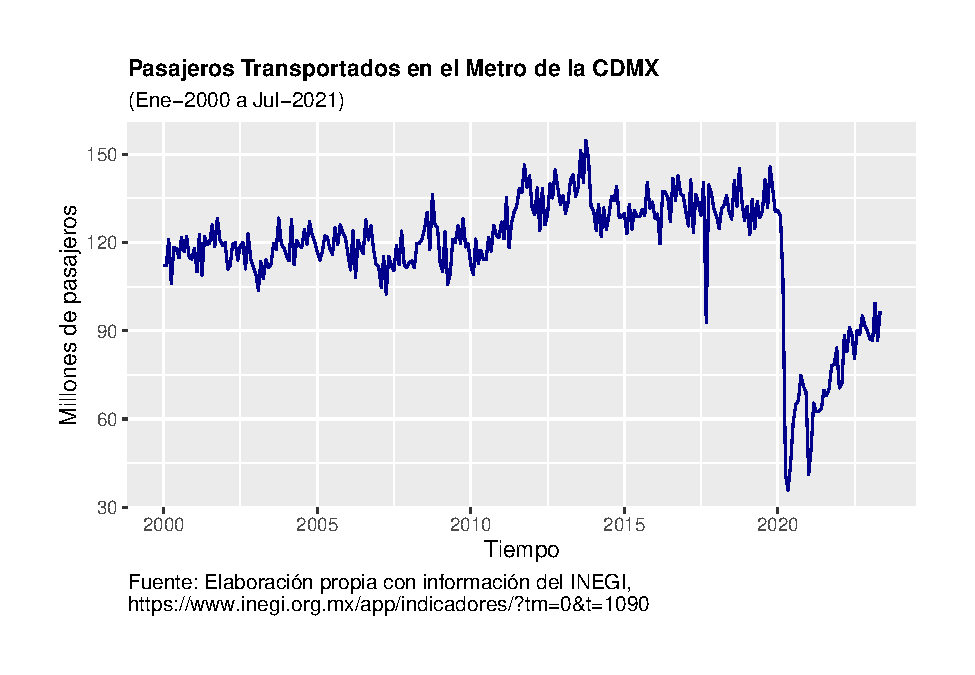
\includegraphics{Notas-Series-Tiempo_files/figure-latex/fig32-1} 

}

\caption{Evolución del número de pasajeros en el Metro de la CDMX, enero 2000 a mayo 2023}\label{fig:fig32}
\end{figure}

\begin{Shaded}
\begin{Highlighting}[]
\CommentTok{\#}
\FunctionTok{ggsave}\NormalTok{(}\StringTok{"Pax\_Metro.png"}\NormalTok{, }\AttributeTok{width =} \DecValTok{20}\NormalTok{, }\AttributeTok{height =} \DecValTok{15}\NormalTok{, }\AttributeTok{units =} \StringTok{"cm"}\NormalTok{)}
\end{Highlighting}
\end{Shaded}

A esta serie de tiempo le calculamos los pincipales estadísticos hasta ahora estudiados y obtenemos el Cuadro \ref{tab:foo}. En dicho cuadro se destaca que se muestra la función de autocirrelación para los tres primeros rezagos. Para mayor detalle, en la Figura \ref{fig:fig33} se muestra la función de autocorrelación, en donde las bandas descritas por las líneas azules son el intervalo de confianza desntro de las cuales no se puede rechazar la hipotésis nula de que \(H_0: \hat{\rho}(p) = 0\), para todo \(\tau = 1, 2, \ldots, T-1\).

\begin{longtable}[]{@{}
  >{\centering\arraybackslash}p{(\columnwidth - 2\tabcolsep) * \real{0.5000}}
  >{\centering\arraybackslash}p{(\columnwidth - 2\tabcolsep) * \real{0.5000}}@{}}
\caption{\label{tab:foo} Estadísticas descriptivas del número de pasajeros en el Metro de la CDMX, enero de 200 a junio de 2019}\tabularnewline
\toprule\noalign{}
\begin{minipage}[b]{\linewidth}\centering
Estadística
\end{minipage} & \begin{minipage}[b]{\linewidth}\centering
Valor
\end{minipage} \\
\midrule\noalign{}
\endfirsthead
\toprule\noalign{}
\begin{minipage}[b]{\linewidth}\centering
Estadística
\end{minipage} & \begin{minipage}[b]{\linewidth}\centering
Valor
\end{minipage} \\
\midrule\noalign{}
\endhead
\bottomrule\noalign{}
\endlastfoot
\(\hat{\mu} = \frac{1}{T} \sum^T_{t=1} X_t\) & 124.3000 \\
\(\hat{\gamma}(0) = \frac{1}{T} \sum^T_{t=1} (X_t - \hat{\mu})^2\) & 103.6400 \\
\(\hat{\gamma}(1) = \frac{1}{T} \sum^{T - 1}_{t=1} (X_t - \hat{\mu})(X_{t+1} - \hat{\mu})\) & 63.1100 \\
\(\hat{\gamma}(2) = \frac{1}{T} \sum^{T - 2}_{t=1} (X_t - \hat{\mu})(X_{t+2} - \hat{\mu})\) & 72.9100 \\
\(\hat{\gamma}(3) = \frac{1}{T} \sum^{T - 3}_{t=1} (X_t - \hat{\mu})(X_{t+3} - \hat{\mu})\) & 63.6900 \\
\(\hat{\rho}(1) = \frac{\sum^{T - 1}_{t=1} (X_t - \hat{\mu})(X_{t+1} - \hat{\mu})}{\sum^T_{t=1} (X_t - \hat{\mu})^2} = \frac{\hat{\gamma}(1)}{\hat{\gamma}(0)}\) & 0.6089 \\
\(\hat{\rho}(2) = \frac{\sum^{T - 2}_{t=1} (X_t - \hat{\mu})(X_{t+2} - \hat{\mu})}{\sum^T_{t=1} (X_t - \hat{\mu})^2} = \frac{\hat{\gamma}(2)}{\hat{\gamma}(0)}\) & 0.7035 \\
\(\hat{\rho}(3) = \frac{\sum^{T - 3}_{t=1} (X_t - \hat{\mu})(X_{t+3} - \hat{\mu})}{\sum^T_{t=1} (X_t - \hat{\mu})^2} = \frac{\hat{\gamma}(3)}{\hat{\gamma}(0)}\) & 0.6145 \\
\(Q^* = T \sum_{j = 1}^{1} \hat{\rho} (j)^2\) & 86.7577 \\
\(Q^* = T \sum_{j = 1}^{2} \hat{\rho} (j)^2\) & 290.9279 \\
\end{longtable}

\begin{Shaded}
\begin{Highlighting}[]
\NormalTok{Pax\_Metro }\OtherTok{\textless{}{-}} \FunctionTok{ts}\NormalTok{(Datos}\SpecialCharTok{$}\NormalTok{Pax\_Metro, }
                \AttributeTok{start =} \DecValTok{2000}\NormalTok{, }
                \AttributeTok{freq =} \DecValTok{12}\NormalTok{)}

\FunctionTok{acf}\NormalTok{(Pax\_Metro, }
    \AttributeTok{lag.max =} \DecValTok{150}\NormalTok{, }
    \AttributeTok{xlab =} \StringTok{\textquotesingle{}Resagos k en meses\textquotesingle{}}\NormalTok{, }
    \AttributeTok{main=}\StringTok{"Funcion de Autocorrelación del número de pasajeros del metro"}\NormalTok{)}
\end{Highlighting}
\end{Shaded}

\begin{figure}

{\centering 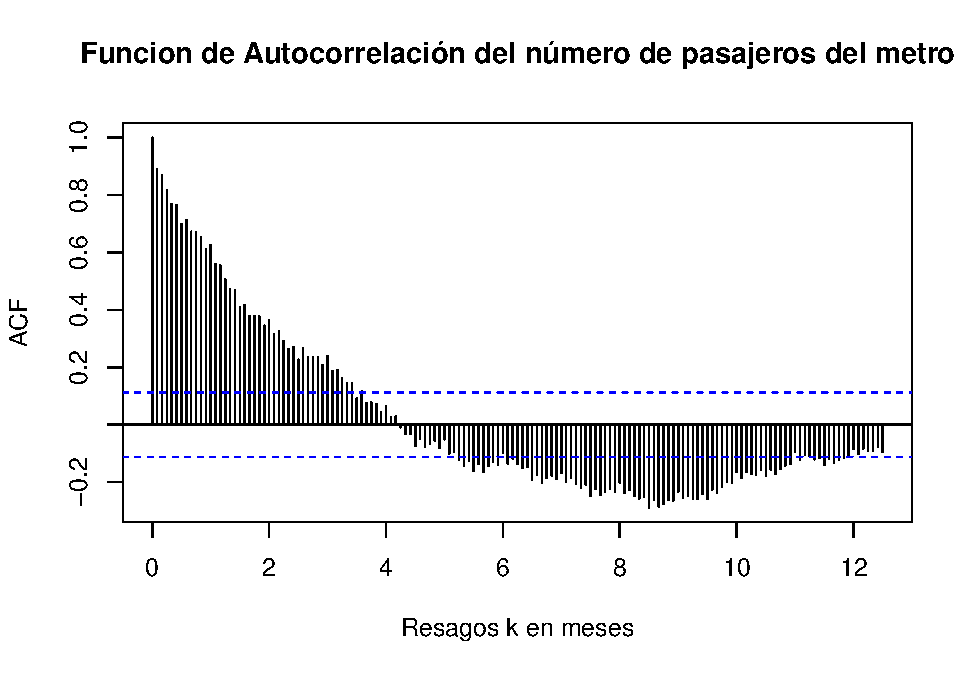
\includegraphics{Notas-Series-Tiempo_files/figure-latex/fig33-1} 

}

\caption{unción de Autocorrelación: 150 rezagos del número de pasajeros en el Metro de la CDMX, enero de 2000 a mayo de 2023}\label{fig:fig33}
\end{figure}

\hypertarget{procesos-estacionarios-univariados}{%
\chapter{Procesos estacionarios univariados}\label{procesos-estacionarios-univariados}}

En este capítulo analizaremos el método o metodología de análisis de series de tiempo propuesto por Box y Jenkins (1970). Los modelos propuestos dentro de está metodología o conjunto de métodos se han vuelto indispensables para efectos de realizar pronósticos de corto plazo.

En este sentido, se analizarán los métodos más importantes en series de tiempo: procesos autoregresivos (AR) y procesos de medias móviles (MA). Asimismo, se realizará un análisis de los procesos que resultan de la combinación de ambos, conocida como ARMA, los cuales son más comúnmente usados para realizar pronósticos.

\hypertarget{procesos-autoregresivos-ar}{%
\section{Procesos Autoregresivos (AR)}\label{procesos-autoregresivos-ar}}

Los procesos autoregresivos tienen su origen en el trabajo de Cochrane y Orcutt de 1949, mediante el cual analizaron los residuales de una regresión clásica como un proceso autoregresivo. Puede consultarse el apéndice para la discusión del modelo de regresión clásica.

\hypertarget{ar1}{%
\subsection{AR(1)}\label{ar1}}

Como primer caso analizaremos al proceso autoregresivo de primer orden, \(AR(1)\), el cual podemos definir como una Ecuación Lineal en Diferencia Estocástica de Primer Orden. Diremos que una Ecuación Lineal en Diferencia de Primer Orden es estocástica si en su representación analítica considera un componente estocástico como en la ecuación (\ref{EDO_Est}) descrita a continuación:
\begin{equation}
    X_t = a_0 + a_1 X_{t-1} + U_t
    \label{EDO_Est}
\end{equation}

Donde \(a_0\) es un término constante, \(U_t\) es un proceso estacionario, con media cero (0), una varianza finita y constante (\(\sigma^2\)) y una covarianza que depende de la distancia entre \(t\) y cualquier \(t-s\) (\(\gamma_s\))--que no depende de los valores pasados o futuros de la variable--, \(X_0\) es el valor inicial del proceso \(X_t\). No obstante, en ocasiones vamos a asumir que la covarianza será cero (0), por lo que en esos casos tendremos un proceso puramente aleatorio. Considerando la ecuación (\ref{EDO_Est} y un proceso de sustitución sucesivo podemos establecer lo siguiente, empezando con \(X_1\):
\begin{eqnarray*}
    X_{1} & = & a_0 + a_1 X_{0} + U_{1}
\end{eqnarray*}

Para \(X_2\):
\begin{eqnarray*}
X_{2} & = & a_0 + a_1 X_{1} + U_{2} \\
    & = & a_0 + a_1 (a_0 + a_1 X_{0} + U_{1}) + U_{2} \\
    & = & a_0 + a_1 a_0 + a_1^2 X_{0} + a_1 U_{1} + U_{2}
\end{eqnarray*}

Para \(X_3\):
\begin{eqnarray*}
X_{3} & = & a_0 + \alpha X_{2} + U_{3} \\
    & = & a_0 + a_1 (a_0 + a_1 a_0 + a_1^2 X_{0} + a_1 U_{1} + U_{2}) + U_{3} \\
    & = & a_0 + a_1 a_0 + a_1^2 a_0 + a_1^3 X_{0} + a_1^2 U_{1} + a_1 U_{2} + U_{3}
\end{eqnarray*}

Así, para cualquier \(X_t\), \(t = 1, 2, 3, \ldots\), obtendríamos:
\begin{eqnarray}
X_{t} & = & a_0 + a_1 X_{t - 1} + U_{t} \nonumber \\
    & = & a_0 + a_1 (a_0 + a_1 a_0 + a_1^2 a_0 + \ldots + a_1^{t-2} a_0 + a_1^{t-1} X_{0} \nonumber \\
    &   & + a_1^{t-2} U_{1} + \ldots + a_1 U_{t - 2} + U_{t - 1}) + U_{t} \nonumber \\
    & = & a_0 + a_1 a_0 + a_1^2 a_0 + a_1^3 a_0 + \ldots + a_1^{t-1} a_0 + a_1^{t} X_{0} \nonumber \\
    &   & + a_1^{t-1} U_{1} + \ldots a_1^2 U_{t - 2} + a_1 U_{t - 1} + U_{t} \nonumber \\
    & = & (1 + a_1 + a_1^2 + a_1^3 + \ldots + a_1^{t-1}) a_0 + a_1^{t} X_{0} \nonumber \\
    &   & + a_1^{t-1} U_{1} + \ldots + a_1^2 U_{t - 2} + a_1 U_{t - 1} + U_{t}  \nonumber\\
    & = & \frac{1 - a_1^t}{1 - a_1} a_0 + a_1^{t} X_{0} + \sum^{t-1}_{j = 0} a_1^{j} U_{t - j} 
    \label{EDO_S_Sol}
\end{eqnarray}

De esta forma en la ecuación (\ref{EDO_S_Sol}) observamos un proceso que es explicado por dos partes: una que depende del tiempo y otra que depende de un proceso estocástico. Asimismo, debe notarse que la condición de convergencia es idéntica que en el caso de ecuaciones en diferencia estudiadas al inicio del curso: \$ \textbar a\_1\textbar{} \textless{} 1\$, por lo que cuando \(t \to \infty\), la expresión (\ref{EDO_S_Sol}) será la siguiente:
\begin{equation}
    X_t = a_0 \frac{1}{1 - a_1} + \sum^{\infty}_{j = 0} a_1^{j} U_{t - j}
    \label{EDO_S_LP}
\end{equation}

Así, desaparece la parte dependiente del tiempo y únicamente prevalece la parte que es dependiente del proceso estocástico. Esta es la solución de largo plazo del proceso \(AR(1)\), la cual depende del proceso estocástico. Notemos, además, que esta solución implica que la variable o la serie de tiempo \(X_t\) es tambien un proceso estocástico que hereda las propiedades de \(U_t\). Así, \(X_t\) es también un proceso estocástico estacionario, como demostraremos más adelante.

Observemos que la ecuación (\ref{EDO_S_LP}) se puede reescribir si consideramos la formulación que en la literatura se denomina como la descomposición de Wold, en la cual se define que es posible asumir que \(\psi_j = a_1^j\) y se considera el caso en el cual \$ \textbar a\_1\textbar{} \textless{} 1 \$, de esta forma tendremos que por ejemplo cuando:
\begin{equation*}
    \sum^{\infty}_{j = 0} \psi^2_j = \sum^{\infty}_{j = 0} a_1^{2j} = \frac{1}{1 - a_1^2} 
\end{equation*}

Alternativamente y de forma similar a las ecuaciones en diferencia estudiadas previamente podemos escribir el proceso \(AR(1)\) mediante el uso del operador rezago como:
\begin{eqnarray}
    X_t & = & a_0 + a_1 L X_t + U_t \nonumber \\
    X_t - a_1 L X_t & = & a_0 + U_t \nonumber \\
    (1 - a_1 L) X_t & = & a_0 + U_t \nonumber \\
    X_t & = & \frac{a_0}{1 - a_1 L} + \frac{1}{1 - a_1 L} U_t
    \label{AR_1}
\end{eqnarray}

En esta última ecuación retomamos el siguiente término para reescribirlo como:
\begin{equation}
    \frac{1}{1 - a_1 L} = 1 + a_1 L + a_1^2 L^2 + a_1^3 L^3 + \ldots 
\end{equation}

Tomando este resultado para sustituirlo en ecuación (\ref{AR_1}), obtenemos la siguiente expresión:
\begin{eqnarray}
X_t & = & (1 + a_1 L + a_1^2 L^2 + a_1^3 L^3 + \ldots) a_0 + (1 + a_1 L + a_1^2 L^2 + a_1^3 L^3 + \ldots) U_t \nonumber \\
    & = & (1 + a_1 + a_1^2 + a_1^3 + \ldots) a_0 + U_t + a_1 U_{t-1} + a_1^2 U_{t-2} + a_1^3 U_{t-3} + \ldots \nonumber \\
    & = & \frac{a_0}{1 - a_1} + \sum^{\infty}_{j = 0} a_1^j U_{t-j}
    \label{AR1_Sol}
\end{eqnarray}

Donde la condición de convergencia y estabilidad del proceso descrito en esta ecuación es que \$ \textbar a\_1\textbar{} \textless{} 1 \$. Por lo que hemos demostrado que mediante el uso del operador de rezago es posible llegar al mismo resultado que obtuvimos mediante el procedimiento de sustituciones iterativas.

La ecuación (\ref{AR1_Sol}) se puede interpretar como sigue. La solución o trayectoria de equilibrio de un AR(1) se divide en dos partes. La primera es una constante que depende de los valores de \(a_0\) y \(a_1\). La segunda parte es la suma ponderada de las desviaciones o errores observados y acumulados en el tiempo hasta el momento \(t\).

Ahora obtendremos los momentos que describen a la serie de tiempo cuando se trata de un porceso \(AR(1)\). Para ello debemos obtener la media, la varianza y las covarianzas de \(X_t\). Para los siguientes resultados debemos recordar y tener en mente que si \(U_t\) es un proceso puramente aleatorio, entonces:

\begin{enumerate}
    \item $\mathbb{E}[U_t] = 0$ para todo $t$
    \item $Var[U_t] = \sigma^2$ para todo $t$
    \item $Cov[U_t, U_s] = 0$ para todo $t \neq s$
\end{enumerate}

Dicho lo anterior y partiendo de la ecuación (\ref{AR1_Sol}), el primer momento o valor esperado de la serie de tiempo será el siguiente:
\begin{eqnarray}
\mathbb{E}[X_t] & = & \mathbb{E} \left[ \frac{a_0}{1 - a_1} + \sum^{\infty}_{j = 0} a_1^j U_{t-j} \right] \nonumber \\
    & = & \frac{a_0}{1 - a_1} + \sum^{\infty}_{j = 0} a_1^j \mathbb{E}[U_{t-j}] \nonumber \\
    & = & \frac{a_0}{1 - a_1} = \mu
    \label{AR1_m1}
\end{eqnarray}

Respecto de la varianza podemos escribir la siguiente expresión a partir de la ecuación (\ref{AR1_Sol}):
\begin{eqnarray}
Var[X_t] & = & \mathbb{E}[(X_t - \mu)^2] \nonumber \\
    & = & \mathbb{E} \left[ \left( \frac{a_0}{1 - a_1} + \sum^{\infty}_{j = 0} a_1^j U_{t-j} - \frac{a_0}{1 - a_1} \right)^2 \right] \nonumber \\
    & = & \mathbb{E}[(U_{t} + a_1 U_{t-1} + a_1^2 U_{t-2} + a_1^3 U_{t-3} + \ldots)^2] \nonumber \\
    & = & \mathbb{E}[U^2_{t} + a_1^2 U^2_{t-1} + a_1^4 U^2_{t-2} + a_1^6 U^2_{t-3} + \ldots \nonumber \\
    &   & + 2 a_1 U_t U_{t-1} + 2 a_1^2 U_t U_{t-2} + \ldots] \nonumber \\
    & = & \mathbb{E}[U^2_{t}] + a_1^2 \mathbb{E}[U^2_{t-1}] + a_1^4 \mathbb{E}[U^2_{t-2}] + a_1^6 \mathbb{E}[U^2_{t-3}] + \ldots \nonumber \\
    & = & \sigma^2 + a_1^2 \sigma^2 + a_1^4 \sigma^2 + a_1^6 \sigma^2 + \ldots \nonumber \\
    & = & \sigma^2 (1 + a_1^2 + a_1^4 + a_1^6 + \ldots) \nonumber \\
    & = & \sigma^2 \frac{1}{1 - a_1^2} = \gamma(0)
    \label{AR1_Var}
\end{eqnarray}

Previo a analizar la covarianza de la serie recordemos que para el proceso puramente aleatorio \(U_t\) su varianza y covarianza puede verse como \(\mathbb{E}[U_t, U_s] = \sigma^2\), para \(t = s\), y \(\mathbb{E}[U_t, U_s] = 0\), para cualquier otro caso, respectivamente.

Dicho lo anterior, partiendo de la ecuación (\ref{AR1_Sol}) la covarianza de la serie estará dada por:
\begin{eqnarray}
Cov(X_t, X_{t-\tau}) & = & \mathbb{E}[(X_t - \mu)(X_{t-\tau} - \mu)] \nonumber \\
    & = & \mathbb{E} \left[ \left( \frac{a_0}{1 - a_1} + \sum^{\infty}_{j = 0} a_1^j U_{t-j} - \frac{a_0}{1 - a_1} \right) \right. \nonumber \\
    &   & \left. \times \left( \frac{a_0}{1 - a_1} + \sum^{\infty}_{j = 0} a_1^j U_{t-\tau-j} - \frac{a_0}{1 - a_1} \right) \right] \nonumber \\
    & = & a_1^{\tau} \mathbb{E}[U^2_{t-\tau} + a_1 U^2_{t-\tau-1} + a_1^2 U^2_{t-\tau-2} + a_1^3 U^2_{t-\tau-3} + \ldots] \nonumber \\
    & = & a_1^{\tau} \sigma^2 \frac{1}{1 - a_1^2} = \gamma(\tau)
    \label{AR1_Cov}
\end{eqnarray}

Notése que con estos resultados en las ecuaciones (\ref{AR1_Var}) y (\ref{AR1_Cov}) podemos construir la función de autocorrelación teórica como sigue:
\begin{eqnarray}
\rho(\tau) & = & \frac{\gamma(\tau)}{\gamma(0)} \nonumber \\
    & = & a_1^\tau
\end{eqnarray}

Donde \(\tau = 1, 2, 3, \ldots\) y \$ \textbar a\_1\textbar{} \textless{} 1\$. Este último resultado significa que cuando el proceso autoregresivo es de orden 1 (es decir, AR(1)) la función de autocorrelación teóricamente es igual al parámetro \(a_1\) elevado al número de rezagos considerados. No obstante, note que esto no significa que la autocorrelación observada sea como lo expresa en planteamiento anterior. Por el contrario, una observación sencilla mostraría que la autocorrelación observada sería ligeramente distinta a la autocorrelación teórica.

Ahora veámos algunos ejemplos. En el primer ejemplo simularemos una serie y mostraremos el analísis de un proceso construído considerando un proceso puramente aleatorio como componente \(U_t\).\footnote{ El procedimiento e implementación del ejercicio está en el archivo R denominado Clase 4 del repositorio de GitHub.} Por su parte, en un segundo ejemplo aplicaremos el análisis a una serie de tiempo de una variable económica observada.\footnote{ El procedimiento e implementación del ejercicio está en el archivo R denominado Clase 5 del repositorio de GitHub.}

Para el primer ejemplo consideremos un proceso dado por la forma de un \(AR(1)\) como en la ecuación (\ref{AR_1}) cuya solución esta dada por la ecuación (\ref{AR1_Sol}). En especifico, supongamos que el término o componente estocástico \(U_t\) es una serie generada a partir de numeros aleatorios de una función normal con media \(0\) y desviación estándar \(4\). Los detalles del proceso simulado se muestra en las siguientes gráficas.

La Figura \ref{fig:fig41} ilustra el comportamiento que se debería observar en una serie considerando el procedimiento iterativo de construcción. Por su parte, la Figura \ref{fig:fig42}\} ilustra el proceso o trayectoria de la solución de la serie de tiempo. Finalmente, las Figuras \ref{fig:fig43}\} y \ref{fig:fig44}\} muestran el correlograma calculado considerando una función de autocorrelación aplicada al porceso real y una función de autocorrelación aplicada al proceso teórico, respectivamente.

\begin{Shaded}
\begin{Highlighting}[]
\FunctionTok{library}\NormalTok{(ggplot2)}
\FunctionTok{library}\NormalTok{(dplyr)}
\FunctionTok{library}\NormalTok{(latex2exp)}

\NormalTok{a0 }\OtherTok{\textless{}{-}} \DecValTok{5}\NormalTok{; a1 }\OtherTok{\textless{}{-}} \FloatTok{0.9}\NormalTok{; X\_0 }\OtherTok{\textless{}{-}}\NormalTok{ (a0}\SpecialCharTok{/}\NormalTok{(}\DecValTok{1} \SpecialCharTok{{-}}\NormalTok{ a1)); T }\OtherTok{\textless{}{-}} \DecValTok{1000}

\NormalTok{X\_t }\OtherTok{\textless{}{-}} \FunctionTok{data.frame}\NormalTok{(}\AttributeTok{Tiempo =} \FunctionTok{c}\NormalTok{(}\DecValTok{0}\SpecialCharTok{:}\NormalTok{T))}


\FunctionTok{set.seed}\NormalTok{(}\DecValTok{12345}\NormalTok{)}

\CommentTok{\# Agregamos un término estocástico al data frame}

\NormalTok{X\_t}\SpecialCharTok{$}\NormalTok{U\_t }\OtherTok{\textless{}{-}} \FunctionTok{rnorm}\NormalTok{(T}\SpecialCharTok{+}\DecValTok{1}\NormalTok{, }\AttributeTok{mean =} \DecValTok{0}\NormalTok{, }\AttributeTok{sd =} \DecValTok{4}\NormalTok{)}

\CommentTok{\# Agregamos columnas con NA\textquotesingle{}s para un proceso teorico y uno real}
\NormalTok{X\_t}\SpecialCharTok{$}\NormalTok{X\_t }\OtherTok{\textless{}{-}} \ConstantTok{NA}
\NormalTok{X\_t}\SpecialCharTok{$}\NormalTok{XR\_t }\OtherTok{\textless{}{-}} \ConstantTok{NA}

\CommentTok{\# La serie teórica inicia en un valor inicial X\_0}
\NormalTok{X\_t}\SpecialCharTok{$}\NormalTok{X\_t[}\DecValTok{1}\NormalTok{] }\OtherTok{\textless{}{-}}\NormalTok{ X\_0}

\CommentTok{\# La serie real inicia en un valor inicial X\_0}
\NormalTok{X\_t}\SpecialCharTok{$}\NormalTok{XR\_t[}\DecValTok{1}\NormalTok{] }\OtherTok{\textless{}{-}}\NormalTok{ X\_0}

\CommentTok{\# Agregamos una columna para la función de Autocorrelación teórica:}
\NormalTok{X\_t}\SpecialCharTok{$}\NormalTok{rho }\OtherTok{\textless{}{-}}\ConstantTok{NA}

\ControlFlowTok{for}\NormalTok{ (i }\ControlFlowTok{in} \DecValTok{2}\SpecialCharTok{:}\NormalTok{(T }\SpecialCharTok{+} \DecValTok{1}\NormalTok{)) \{}
  \CommentTok{\# Real:}
\NormalTok{  X\_t}\SpecialCharTok{$}\NormalTok{XR\_t[i] }\OtherTok{=}\NormalTok{ a0 }\SpecialCharTok{+}\NormalTok{ a1}\SpecialCharTok{*}\NormalTok{X\_t}\SpecialCharTok{$}\NormalTok{XR\_t[i}\DecValTok{{-}1}\NormalTok{] }\SpecialCharTok{+}\NormalTok{ X\_t}\SpecialCharTok{$}\NormalTok{U\_t[i}\DecValTok{{-}1}\NormalTok{]}
  
  \CommentTok{\# Teórico:}
\NormalTok{  X\_t}\SpecialCharTok{$}\NormalTok{X\_t[i] }\OtherTok{=}\NormalTok{ X\_t}\SpecialCharTok{$}\NormalTok{X\_t[i}\DecValTok{{-}1}\NormalTok{] }\SpecialCharTok{+}\NormalTok{ (a1}\SpecialCharTok{\^{}}\NormalTok{(i}\DecValTok{{-}1}\NormalTok{))}\SpecialCharTok{*}\NormalTok{X\_t}\SpecialCharTok{$}\NormalTok{U\_t[i}\DecValTok{{-}1}\NormalTok{]}
  
  \CommentTok{\# Autocorrelación:}
\NormalTok{  X\_t}\SpecialCharTok{$}\NormalTok{rho[i}\DecValTok{{-}1}\NormalTok{] }\OtherTok{=}\NormalTok{ a1}\SpecialCharTok{\^{}}\NormalTok{(i}\DecValTok{{-}1}\NormalTok{)}
\NormalTok{\}}

\FunctionTok{ggplot}\NormalTok{(}\AttributeTok{data =}\NormalTok{ X\_t, }\FunctionTok{aes}\NormalTok{(}\AttributeTok{x =}\NormalTok{ Tiempo, }\AttributeTok{y =}\NormalTok{ XR\_t)) }\SpecialCharTok{+} 
  \FunctionTok{geom\_line}\NormalTok{(}\AttributeTok{size =} \FloatTok{0.5}\NormalTok{, }\AttributeTok{color =} \StringTok{"darkred"}\NormalTok{) }\SpecialCharTok{+}
  \CommentTok{\#theme\_bw() + }
  \FunctionTok{xlab}\NormalTok{(}\StringTok{"Tiempo"}\NormalTok{) }\SpecialCharTok{+} 
  \FunctionTok{ylab}\NormalTok{(}\FunctionTok{TeX}\NormalTok{(}\StringTok{"$X\_t$"}\NormalTok{)) }\SpecialCharTok{+} 
  \FunctionTok{theme}\NormalTok{(}\AttributeTok{plot.title =} \FunctionTok{element\_text}\NormalTok{(}\AttributeTok{size =} \DecValTok{11}\NormalTok{, }\AttributeTok{face =} \StringTok{"bold"}\NormalTok{, }\AttributeTok{hjust =} \DecValTok{0}\NormalTok{)) }\SpecialCharTok{+} 
  \FunctionTok{theme}\NormalTok{(}\AttributeTok{plot.subtitle =} \FunctionTok{element\_text}\NormalTok{(}\AttributeTok{size =} \DecValTok{10}\NormalTok{, }\AttributeTok{hjust =} \DecValTok{0}\NormalTok{)) }\SpecialCharTok{+} 
  \FunctionTok{theme}\NormalTok{(}\AttributeTok{plot.caption =} \FunctionTok{element\_text}\NormalTok{(}\AttributeTok{size =} \DecValTok{10}\NormalTok{, }\AttributeTok{hjust =} \DecValTok{0}\NormalTok{)) }\SpecialCharTok{+}
  \FunctionTok{theme}\NormalTok{(}\AttributeTok{plot.margin =} \FunctionTok{unit}\NormalTok{(}\FunctionTok{c}\NormalTok{(}\DecValTok{1}\NormalTok{,}\DecValTok{1}\NormalTok{,}\DecValTok{1}\NormalTok{,}\DecValTok{1}\NormalTok{), }\StringTok{"cm"}\NormalTok{)) }\SpecialCharTok{+}
  \FunctionTok{labs}\NormalTok{(}
    \AttributeTok{title =} \StringTok{"Comportamiento del Proceso Real (\textquotesingle{}Estimado\textquotesingle{})"}\NormalTok{,}
    \AttributeTok{subtitle =} \StringTok{"Con un error con Distribución Normal (media = 0, desviación estándar = 4)"}\NormalTok{,}
    \AttributeTok{caption =} \StringTok{"Fuente: Elaboración propia."}
\NormalTok{  )}
\end{Highlighting}
\end{Shaded}

\begin{verbatim}
## Warning: Using `size` aesthetic for lines was deprecated in ggplot2 3.4.0.
## i Please use `linewidth` instead.
## This warning is displayed once every 8 hours.
## Call `lifecycle::last_lifecycle_warnings()` to see where this warning was
## generated.
\end{verbatim}

\begin{figure}

{\centering 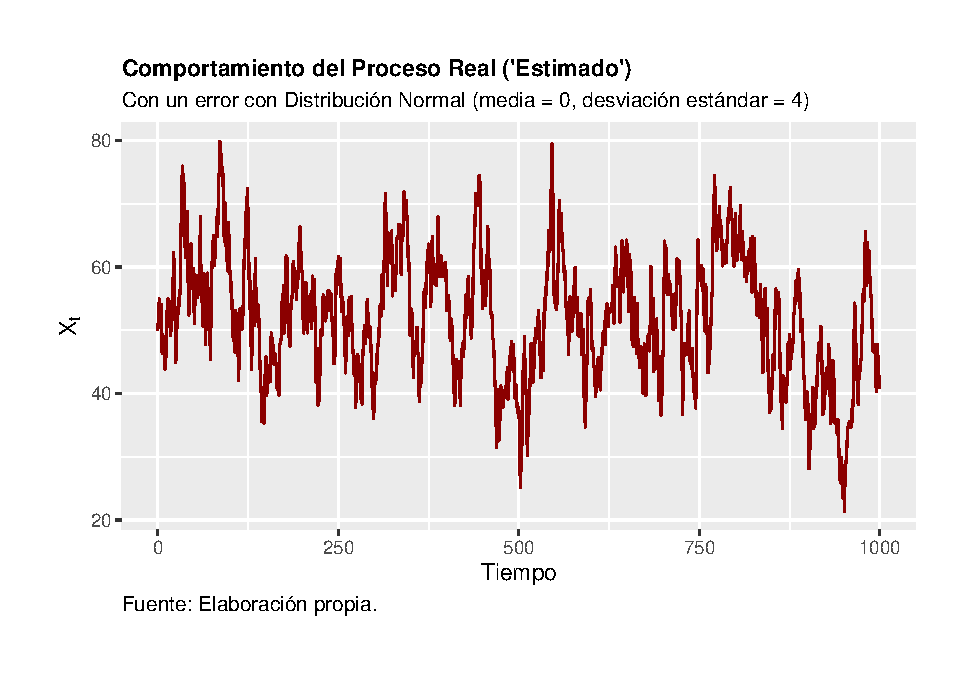
\includegraphics{Notas-Series-Tiempo_files/figure-latex/fig41-1} 

}

\caption{Comportamiento del Proceso Real ('Estimado')}\label{fig:fig41}
\end{figure}

\begin{Shaded}
\begin{Highlighting}[]
\FunctionTok{ggsave}\NormalTok{(}\StringTok{"G\_AR\_1\_Real.png"}\NormalTok{, }\AttributeTok{width =} \DecValTok{20}\NormalTok{, }\AttributeTok{height =} \DecValTok{10}\NormalTok{, }\AttributeTok{units =} \StringTok{"cm"}\NormalTok{)}
\end{Highlighting}
\end{Shaded}

\begin{Shaded}
\begin{Highlighting}[]
\FunctionTok{ggplot}\NormalTok{(}\AttributeTok{data =}\NormalTok{ X\_t, }\FunctionTok{aes}\NormalTok{(}\AttributeTok{x =}\NormalTok{ Tiempo, }\AttributeTok{y =}\NormalTok{ X\_t)) }\SpecialCharTok{+} 
  \FunctionTok{geom\_line}\NormalTok{(}\AttributeTok{size =} \FloatTok{0.5}\NormalTok{, }\AttributeTok{color =} \StringTok{"darkblue"}\NormalTok{) }\SpecialCharTok{+}
  \CommentTok{\#theme\_bw() + }
  \FunctionTok{xlab}\NormalTok{(}\StringTok{"Tiempo"}\NormalTok{) }\SpecialCharTok{+} 
  \FunctionTok{ylab}\NormalTok{(}\FunctionTok{TeX}\NormalTok{(}\StringTok{"$X\_t$"}\NormalTok{)) }\SpecialCharTok{+} 
  \FunctionTok{theme}\NormalTok{(}\AttributeTok{plot.title =} \FunctionTok{element\_text}\NormalTok{(}\AttributeTok{size =} \DecValTok{11}\NormalTok{, }\AttributeTok{face =} \StringTok{"bold"}\NormalTok{, }\AttributeTok{hjust =} \DecValTok{0}\NormalTok{)) }\SpecialCharTok{+} 
  \FunctionTok{theme}\NormalTok{(}\AttributeTok{plot.subtitle =} \FunctionTok{element\_text}\NormalTok{(}\AttributeTok{size =} \DecValTok{10}\NormalTok{, }\AttributeTok{hjust =} \DecValTok{0}\NormalTok{)) }\SpecialCharTok{+} 
  \FunctionTok{theme}\NormalTok{(}\AttributeTok{plot.caption =} \FunctionTok{element\_text}\NormalTok{(}\AttributeTok{size =} \DecValTok{10}\NormalTok{, }\AttributeTok{hjust =} \DecValTok{0}\NormalTok{)) }\SpecialCharTok{+}
  \FunctionTok{theme}\NormalTok{(}\AttributeTok{plot.margin =} \FunctionTok{unit}\NormalTok{(}\FunctionTok{c}\NormalTok{(}\DecValTok{1}\NormalTok{,}\DecValTok{1}\NormalTok{,}\DecValTok{1}\NormalTok{,}\DecValTok{1}\NormalTok{), }\StringTok{"cm"}\NormalTok{)) }\SpecialCharTok{+}
  \FunctionTok{labs}\NormalTok{(}
    \AttributeTok{title =} \StringTok{"Comportamiento del Proceso Teórico"}\NormalTok{,}
    \AttributeTok{subtitle =} \StringTok{"Con un error con Distribución Normal (media = 0, desviación estándar = 4)"}\NormalTok{,}
    \AttributeTok{caption =} \StringTok{"Fuente: Elaboración propia."}
\NormalTok{  )}
\end{Highlighting}
\end{Shaded}

\begin{figure}

{\centering 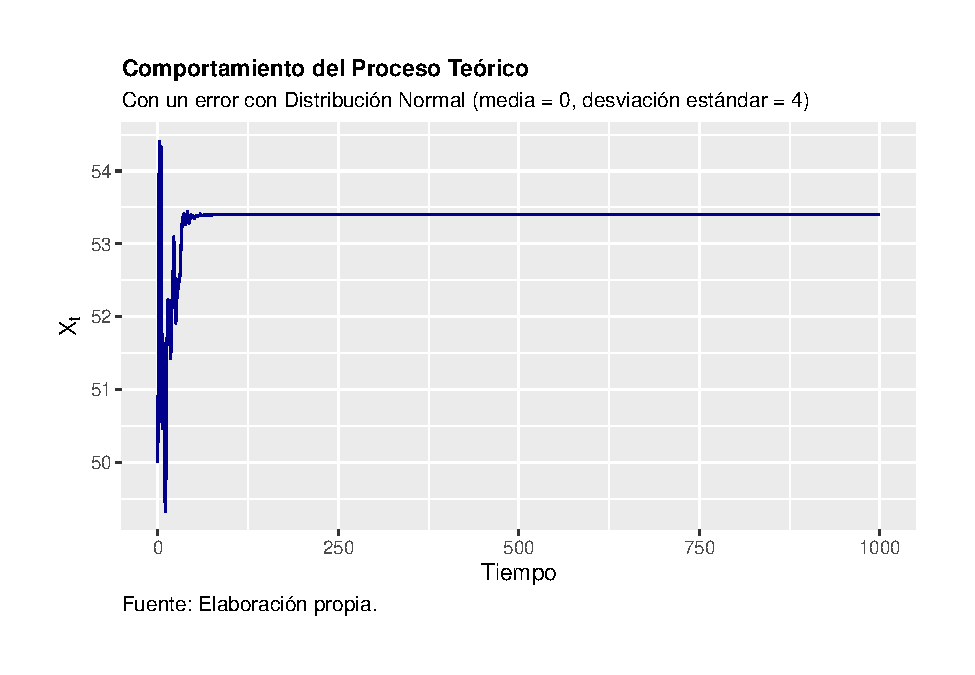
\includegraphics{Notas-Series-Tiempo_files/figure-latex/fig42-1} 

}

\caption{Comportamiento del Proceso Teórico}\label{fig:fig42}
\end{figure}

\begin{Shaded}
\begin{Highlighting}[]
\FunctionTok{ggsave}\NormalTok{(}\StringTok{"G\_AR\_1\_Teo.png"}\NormalTok{, }\AttributeTok{width =} \DecValTok{20}\NormalTok{, }\AttributeTok{height =} \DecValTok{10}\NormalTok{, }\AttributeTok{units =} \StringTok{"cm"}\NormalTok{)}
\end{Highlighting}
\end{Shaded}

\begin{Shaded}
\begin{Highlighting}[]
\FunctionTok{acf}\NormalTok{(X\_t}\SpecialCharTok{$}\NormalTok{XR\_t, }\AttributeTok{lag.max =} \DecValTok{30}\NormalTok{, }\AttributeTok{col =} \StringTok{"blue"}\NormalTok{, }
    \AttributeTok{ylab =} \StringTok{"Autocorrelacion"}\NormalTok{,}
    \AttributeTok{xlab=}\StringTok{"Rezagos"}\NormalTok{, }
    \AttributeTok{main=}\StringTok{"Funcion de Autocorrelacion Real"}\NormalTok{)}
\end{Highlighting}
\end{Shaded}

\begin{figure}

{\centering 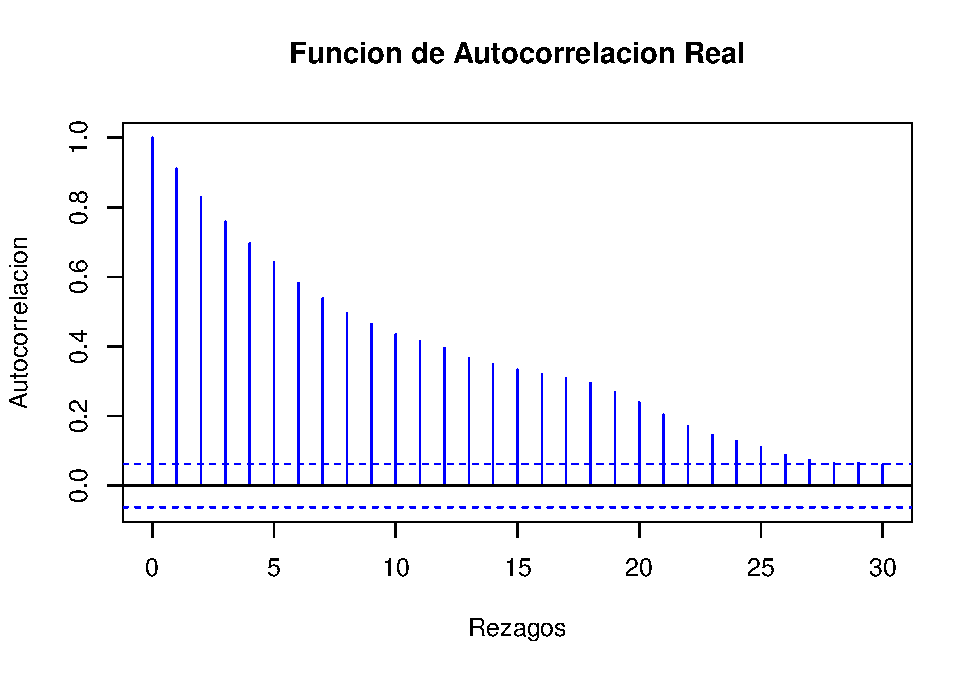
\includegraphics{Notas-Series-Tiempo_files/figure-latex/fig43-1} 

}

\caption{Funcion de Autocorrelacion Real}\label{fig:fig43}
\end{figure}

\begin{Shaded}
\begin{Highlighting}[]
\FunctionTok{barplot}\NormalTok{(X\_t}\SpecialCharTok{$}\NormalTok{rho[}\DecValTok{1}\SpecialCharTok{:}\DecValTok{30}\NormalTok{], }\AttributeTok{names.arg =} \FunctionTok{c}\NormalTok{(}\DecValTok{1}\SpecialCharTok{:}\DecValTok{30}\NormalTok{), }\AttributeTok{col =} \StringTok{"blue"}\NormalTok{, }\AttributeTok{border=}\StringTok{"blue"}\NormalTok{, }\AttributeTok{density =} \FunctionTok{c}\NormalTok{(}\DecValTok{10}\NormalTok{,}\DecValTok{20}\NormalTok{), }
        \AttributeTok{ylab =} \StringTok{"Autocorrelacion"}\NormalTok{, }
        \AttributeTok{xlab=}\StringTok{"Rezagos"}\NormalTok{, }
        \AttributeTok{main=}\StringTok{"Funcion de Autocorrelacion Teórica"}\NormalTok{)}
\end{Highlighting}
\end{Shaded}

\begin{figure}

{\centering 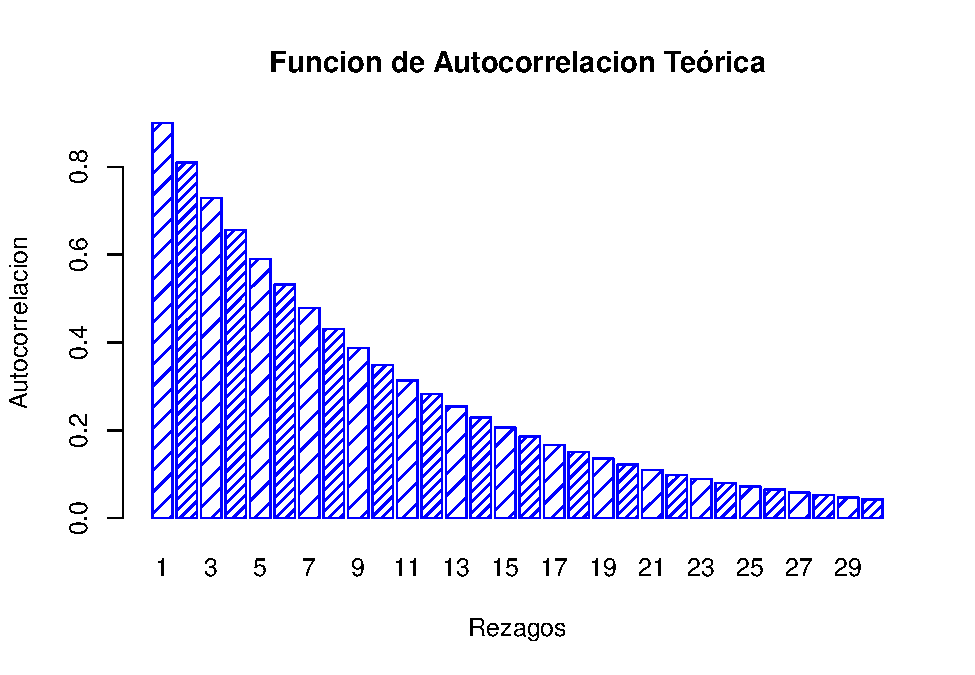
\includegraphics{Notas-Series-Tiempo_files/figure-latex/fig44-1} 

}

\caption{Funcion de Autocorrelacion Teórica}\label{fig:fig44}
\end{figure}

Recordemos que una trayectoria de equilibrio o solución de un \(AR(1)\) es como se muestra en la ecuación (\ref{AR1_Sol}). Así, nuestra serie simulada cumple con la característica de que los errores son más relevantes cuando la serie es corta. Por el contrario, los errores son menos relevantes, cuando la serie es muy larga. La Figura \ref{fig:fig45}\} ilustra esta observación de la trayectoria de equilibrio.

\begin{Shaded}
\begin{Highlighting}[]
\FunctionTok{ggplot}\NormalTok{(}\AttributeTok{data =}\NormalTok{ X\_t, }\FunctionTok{aes}\NormalTok{(}\AttributeTok{x =}\NormalTok{ Tiempo)) }\SpecialCharTok{+}
  \FunctionTok{geom\_line}\NormalTok{(}\FunctionTok{aes}\NormalTok{(}\AttributeTok{y =}\NormalTok{ XR\_t), }\AttributeTok{size =} \FloatTok{0.5}\NormalTok{, }\AttributeTok{color =} \StringTok{"darkred"}\NormalTok{) }\SpecialCharTok{+}
  \FunctionTok{geom\_line}\NormalTok{(}\FunctionTok{aes}\NormalTok{(}\AttributeTok{y =}\NormalTok{ X\_t), }\AttributeTok{size =} \FloatTok{0.5}\NormalTok{, }\AttributeTok{color =} \StringTok{"darkblue"}\NormalTok{) }\SpecialCharTok{+}
  \CommentTok{\#theme\_bw() + }
  \FunctionTok{xlab}\NormalTok{(}\StringTok{"Tiempo"}\NormalTok{) }\SpecialCharTok{+} 
  \FunctionTok{ylab}\NormalTok{(}\FunctionTok{TeX}\NormalTok{(}\StringTok{"$X\_t$"}\NormalTok{)) }\SpecialCharTok{+} 
  \FunctionTok{theme}\NormalTok{(}\AttributeTok{plot.title =} \FunctionTok{element\_text}\NormalTok{(}\AttributeTok{size =} \DecValTok{11}\NormalTok{, }\AttributeTok{face =} \StringTok{"bold"}\NormalTok{, }\AttributeTok{hjust =} \DecValTok{0}\NormalTok{)) }\SpecialCharTok{+} 
  \FunctionTok{theme}\NormalTok{(}\AttributeTok{plot.subtitle =} \FunctionTok{element\_text}\NormalTok{(}\AttributeTok{size =} \DecValTok{10}\NormalTok{, }\AttributeTok{hjust =} \DecValTok{0}\NormalTok{)) }\SpecialCharTok{+} 
  \FunctionTok{theme}\NormalTok{(}\AttributeTok{plot.caption =} \FunctionTok{element\_text}\NormalTok{(}\AttributeTok{size =} \DecValTok{10}\NormalTok{, }\AttributeTok{hjust =} \DecValTok{0}\NormalTok{)) }\SpecialCharTok{+}
  \FunctionTok{theme}\NormalTok{(}\AttributeTok{plot.margin =} \FunctionTok{unit}\NormalTok{(}\FunctionTok{c}\NormalTok{(}\DecValTok{1}\NormalTok{,}\DecValTok{1}\NormalTok{,}\DecValTok{1}\NormalTok{,}\DecValTok{1}\NormalTok{), }\StringTok{"cm"}\NormalTok{)) }\SpecialCharTok{+}
  \FunctionTok{labs}\NormalTok{(}
    \AttributeTok{title =} \StringTok{"Comportamiento de los Procesos Real y Teórico"}\NormalTok{,}
    \AttributeTok{subtitle =} \StringTok{"Con un error con Distribución Normal (media = 0, desviación estándar = 4)"}\NormalTok{,}
    \AttributeTok{caption =} \StringTok{"Fuente: Elaboración propia."}
\NormalTok{  )}
\end{Highlighting}
\end{Shaded}

\begin{figure}

{\centering 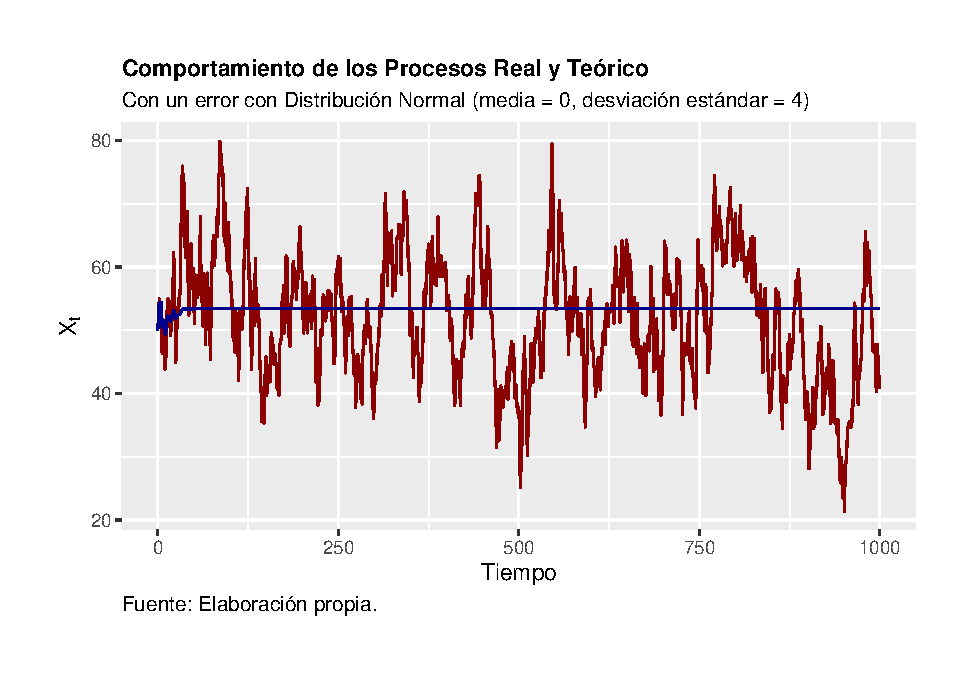
\includegraphics{Notas-Series-Tiempo_files/figure-latex/fig45-1} 

}

\caption{Comportamiento de los Procesos Real y Teórico}\label{fig:fig45}
\end{figure}

\begin{Shaded}
\begin{Highlighting}[]
\FunctionTok{ggsave}\NormalTok{(}\StringTok{"G\_AR\_1\_Comb.png"}\NormalTok{, }\AttributeTok{width =} \DecValTok{20}\NormalTok{, }\AttributeTok{height =} \DecValTok{10}\NormalTok{, }\AttributeTok{units =} \StringTok{"cm"}\NormalTok{)}
\end{Highlighting}
\end{Shaded}

Para el segundo ejemplo consideremos una aplicación a una serie de tiempo en especifico: Pasajeros transportados mensualmente en el Sistema de Transporte Colectivo Metro (pasajeros medidos en millones).\footnote{Fuente: INEGI, \url{https://www.inegi.org.mx/app/indicadores/?tm=0&t=1090}.}

A la serie se le aplicará una metodología de estimación dada por el método de Máxima Verosimilitud (ML, por sus siglás en inglés). Antes de realizar el proceso de estimación consideremos una transformación de diferencias logaritmicas, con el objeto de obtener una serie de tiempo expresada en tasas de crecimiento\footnote{Estas tasas no son porcentuales, para hacerlas porcentuales faltaría multiplicar por 100 cada calor de la serie.} y con un comportamiento parecido a un proceso estacionario.

Así, para cada una de las series que analicemos en diferencias logaritmicas respecto del momento \(k\) las expresaremos bajo la siguiente transformación:
\begin{equation*}
    DLX_t = log(X_t) - log(X_{t-k})
\end{equation*}

Donde \(k = 1, 2, 3, \ldots\) y \(log(.)\) es la función logaritmo natural. Esta expresión se pude interpretar como una tasa de crecimiento puesto que asumimos variaciones pequeñas para las cuales se cumple que: \(log(X_t) - log(X_{t-k}) \approx \frac{X_t - X_{t-k}}{X_t}\).

Primero, para realizar el análisis de una serie de tiempo deberemos decidir si éste se realizará para la serie en niveles o en diferencias. Por convención, decimos que la series esta en niveles si ésta se analiza sin heacerle ninguna transformación o si se analiza aplicando solo logarimos. Cuando la serie se analiza en diferencias significa que la diferencia se hace sin aplicar logaritmos o aplicando logaritmos. Sin embargo, la convención es hacer un análisis en diferencias logaritmicas.

Para decidir cómo analizar la serie de pasajeros en el metro de la CDMX en la Figura \ref{fig:fig46}\} se muestra la gráfica de la serie en niveles (sin transformación logaritmica y con transformación logarítmica) y en diferencias logarítmicas mensuales (es decir, con \(k = 1\)).

\begin{Shaded}
\begin{Highlighting}[]
\FunctionTok{library}\NormalTok{(ggplot2)}
\FunctionTok{library}\NormalTok{(dplyr)}
\FunctionTok{library}\NormalTok{(readxl)}
\FunctionTok{library}\NormalTok{(stats)}

\NormalTok{Datos }\OtherTok{\textless{}{-}} \FunctionTok{read\_excel}\NormalTok{(}\StringTok{"BD/Base\_Transporte.xlsx"}\NormalTok{, }\AttributeTok{sheet =} \StringTok{"Datos"}\NormalTok{, }\AttributeTok{col\_names =} \ConstantTok{TRUE}\NormalTok{)}

\CommentTok{\# En Niveles}
\NormalTok{Pax\_Metro }\OtherTok{\textless{}{-}} \FunctionTok{ts}\NormalTok{(Datos}\SpecialCharTok{$}\NormalTok{Pax\_Metro, }\AttributeTok{start =} \FunctionTok{c}\NormalTok{(}\DecValTok{2000}\NormalTok{, }\DecValTok{1}\NormalTok{), }
                \AttributeTok{freq =} \DecValTok{12}\NormalTok{)}

\CommentTok{\# En Logaritmos:}
\NormalTok{Pax\_LMetro }\OtherTok{\textless{}{-}} \FunctionTok{ts}\NormalTok{(}\FunctionTok{log}\NormalTok{(Datos}\SpecialCharTok{$}\NormalTok{Pax\_Metro), }\AttributeTok{start =} \FunctionTok{c}\NormalTok{(}\DecValTok{2000}\NormalTok{, }\DecValTok{1}\NormalTok{), }
                \AttributeTok{freq =} \DecValTok{12}\NormalTok{)}

\CommentTok{\# Diferencias mensuales:}
\NormalTok{Pax\_DLMetro }\OtherTok{\textless{}{-}} \FunctionTok{ts}\NormalTok{( }\FunctionTok{log}\NormalTok{(Datos}\SpecialCharTok{$}\NormalTok{Pax\_Metro) }\SpecialCharTok{{-}} \FunctionTok{lag}\NormalTok{( }\FunctionTok{log}\NormalTok{(Datos}\SpecialCharTok{$}\NormalTok{Pax\_Metro), }\DecValTok{1}\NormalTok{ ),}
                 \AttributeTok{start =} \FunctionTok{c}\NormalTok{(}\DecValTok{2000}\NormalTok{, }\DecValTok{1}\NormalTok{), }\AttributeTok{freq =} \DecValTok{12}\NormalTok{)}

\CommentTok{\#}
\FunctionTok{par}\NormalTok{(}\AttributeTok{mfrow =} \FunctionTok{c}\NormalTok{(}\DecValTok{3}\NormalTok{,}\DecValTok{1}\NormalTok{))}

\FunctionTok{plot}\NormalTok{(Pax\_Metro, }\AttributeTok{xlab =} \StringTok{"Tiempo"}\NormalTok{, }
     \AttributeTok{main =} \StringTok{"Pasajeros transportados (Millones) en el SCM"}\NormalTok{,}
     \AttributeTok{col =} \StringTok{"darkgreen"}\NormalTok{)}

\FunctionTok{plot}\NormalTok{(Pax\_LMetro, }\AttributeTok{xlab =} \StringTok{"Tiempo"}\NormalTok{, }
     \AttributeTok{main =} \StringTok{"LN Pasajeros transportados (Millones) en el SCM"}\NormalTok{,}
     \AttributeTok{col =} \StringTok{"darkblue"}\NormalTok{)}

\FunctionTok{plot}\NormalTok{(Pax\_DLMetro, }\AttributeTok{xlab =} \StringTok{"Tiempo"}\NormalTok{, }
     \AttributeTok{main =} \StringTok{"Diff LN Pasajeros transportados (Millones) en el SCM"}\NormalTok{, }
     \AttributeTok{col =} \StringTok{"darkred"}\NormalTok{)}
\end{Highlighting}
\end{Shaded}

\begin{figure}

{\centering 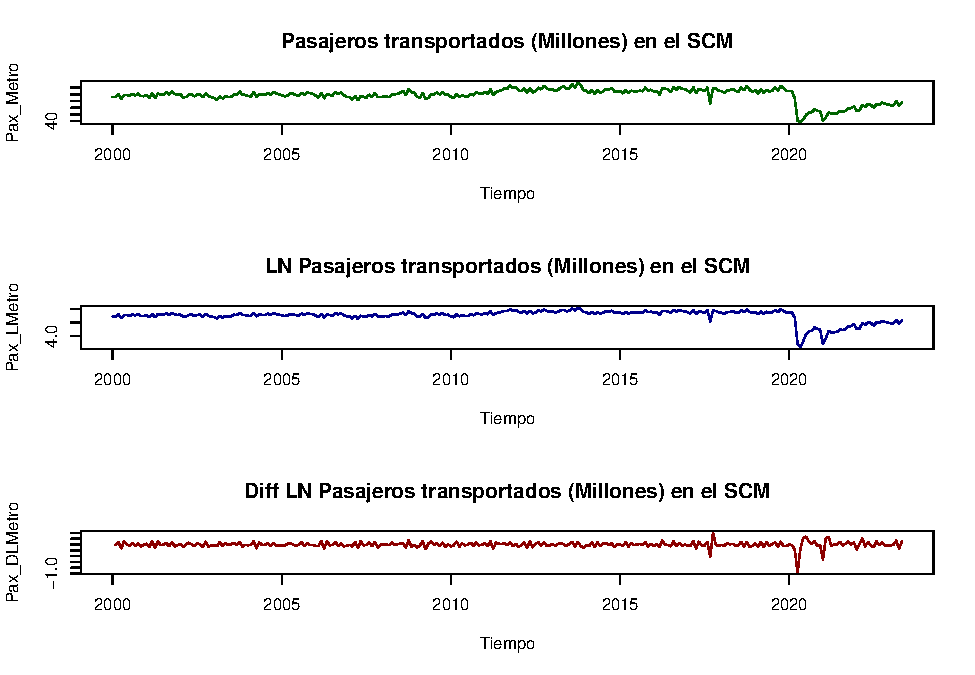
\includegraphics{Notas-Series-Tiempo_files/figure-latex/fig46-1} 

}

\caption{Pasajeros transportados (Millones) en el metro de la CDM en niveles y en diferencias logaritmicas}\label{fig:fig46}
\end{figure}

\begin{Shaded}
\begin{Highlighting}[]
\FunctionTok{par}\NormalTok{(}\AttributeTok{mfrow=}\FunctionTok{c}\NormalTok{(}\DecValTok{1}\NormalTok{,}\DecValTok{1}\NormalTok{))}
\end{Highlighting}
\end{Shaded}

A continuación, estimaremos una \(AR(1)\) para la serie en niveles bajo la transformación logaritmica (\(PaxLMetro_t\)) y en diferencias logarítmitcas (\(PaxDLMetro_t\)). Para el primer caso obtenemos el siguiente resultado:

\begin{center}
\begin{tabular}{ c c c c c c } 
    $PaxLMetro_t$ & $=$ & $4.7419$ & $+$ & $0.5916$  & $PaxLMetro_{t-1}$ \\ 
    &  & $(0.0105)$ &  & $(0.0526)$ & 
\end{tabular}
\end{center}

\begin{center}
\begin{tabular}{ c c c c c c c } 
    $\hat{\sigma}^2$ & $=$ & $0.004335$ & y & $AIC$ & $=$ & $-602.73$ 
\end{tabular}
\end{center}

Para el segundo caso obtenemos el siguiente resultado:

\begin{center}
\begin{tabular}{ c c c c c c } 
    $PaxDLMetro_t$ & $=$ & $0.0007$ & $-$ & $0.6194$  & $PaxDLMetro_{t-1}$ \\ 
    &  & $(0.0023)$ &  & $(0.0511)$ & 
\end{tabular}
\end{center}

\begin{center}
\begin{tabular}{ c c c c c c c } 
    $\hat{\sigma}^2$ & $=$ & $0.003344$ & y & AIC & $=$ & $-660.53$ 
\end{tabular}
\end{center}

En ambos casos observamos que el parámetro asociado al componente AR es significativo y cumple con la restricción de ser en valor absoluto menor a 1, por lo que la solución asociada al procesp será convergente. También en ambos casos se reporta la estadística o Criterio de Información de Akaike (AIC, por sus siglas en inglés), misma que más adelante discutiremos su importancia y aplicación.

\hypertarget{ar2}{%
\subsection{AR(2)}\label{ar2}}

Una vez analizado el caso de \(AR(1)\) analizaremos el caso del \(AR(2)\). La ecuación generalizada del proceso autoregresivo de orden 2 (denotado como \(AR(2)\)) puede ser escrito como:
\begin{equation}
    X_t = a_0 + a_1 X_{t-1} + a_2 X_{t-2} + U_t
    \label{AR2_Eq}
\end{equation}

Donde \(U_t\) denota un proceso puramente aleatorio con media cero (\(0\)), varianza constante (\(\sigma^2\)) y autocovarianza cero (\(Cov(U_t, U_s) = 0\), con \(t \neq s\)), y un parametro \(a_2 \neq 0\). Así, utilizando el operador rezago podemos reescribir la ecuación (\ref{AR2_Eq}) como:
\begin{eqnarray*}
    X_t - a_1 X_{t-1} - a_2 X_{t-2} & = & a_0 + U_t \\
    (1 - a_1 L^1 - a_2 L^2) X_t & = & a_0 + U_t
\end{eqnarray*}

Donde, vamos a denotar a \(\alpha (L) = (1 - a_1 L^1 - a_2 L^2)\), y lo llamaremos como un polinomio que depende del operador rezago y que es distinto de cero. De esta forma podemos reescribir a la ecuación (\ref{AR2_Eq}) como:
\begin{equation}
    \alpha(L) X_t = a_0 + U_t
\end{equation}

Ahora, supongamos que existe el inverso multiplicativo del polinomio \(\alpha(L)\), el cual será denotado como: \(\alpha^{-1}(L)\) y cumple con que:
\begin{equation}
    \alpha^{-1}(L) \alpha(L) = 1    
\end{equation}

Así, podemos escribir la solución a la ecuación (\ref{AR2_Eq}) como:
\begin{equation*}
    X_t = \alpha^{-1}(L) \delta + \alpha^{-1}(L) U_t
\end{equation*}

Si utilizamos el hecho que \(\alpha^{-1}(L)\) se puede descomponer a través del procedimiento de Wold en un polinomio de forma similar el caso de \(AR(1)\), tenemos que:
\begin{equation}
    \alpha^{-1}(L) = \psi_0 + \psi_1 L + \psi_2 L^2 + \ldots
\end{equation}

Por lo tanto, el inverso multiplicativo \(\alpha^{-1}(L)\) se puede ver como:
\begin{equation}
    1 = (1 - a_1 L^1 - a_2 L^2) (\psi_0 + \psi_1 L + \psi_2 L^2 + \ldots)
    \label{InvAlpha}
\end{equation}

Desarrollando la ecuación (\ref{InvAlpha}) tenemos la sigueinte expresión:

\begin{center}
\begin{tabular}{ c c c c c c c c c c c } 
    $1$ & $=$ & $\psi_0$ & $+$ & $\psi_1 L$ & $+$ & $\psi_2 L^2$ & $+$ & $\psi_3 L^3$ & $+$ & $\ldots$ \\
    $ $ & $ $ & $ $ & $-$ & $a_1 \psi_0 L$ & $-$ & $a_1 \psi_1 L^2$ & $-$ & $a_1 \psi_2 L^3$ & $-$ & $\ldots$ \\
    $ $ & $ $ & $ $ & $ $ & $ $ & $-$ & $a_2 \psi_0 L^2 $ & $-$ & $a_2 \psi_1 L^3$ & $-$ & $\ldots$
\end{tabular}
\end{center}

Ahora, podemos agrupar todos los términos en función del exponente asociado al operador rezago \(L\). La siguiente es una solución partícular y es una de las múltiples que podrían existir que cumpla con la ecuación (\ref{InvAlpha}). Sin embargo, para efectos del análisis sólo necesitamos una de esas soluciones. Utilizaremos las siguientes condiciones que deben cumplirse en una de las posibles soluciones:

\begin{center}
\begin{tabular}{ c c c c } 
    $L^0 :$ & $ $ & $\Rightarrow$ & $\psi_0 = 1$ \\
    $L :$ & $\psi_1 - a_1 \psi_0 = 0$ & $\Rightarrow$ & $\psi_1 = a_1$ \\
    $L^2 :$ & $\psi_2 - a_1 \psi_1 - a_2 \psi_0 = 0$ & $\Rightarrow$ & $\psi_2 = a^2_1 + a_2$ \\
    $L^3 :$ & $\psi_3 - a_1 \psi_2 - a_2 \psi_1 = 0$ & $\Rightarrow$ & $\psi_3 = a^3_1 + 2 a_1 a_2$ \\
    $\vdots$ & $\vdots$ & $\vdots$ & $\vdots$
\end{tabular}
\end{center}

De esta forma podemos observar que en el límite siempre obtendremos una ecuación del tipo \(\psi_j - a_1 \psi_{j-1} - a_2 \psi_{j-2} = 0\) asociada a cada uno de los casos en que exista un \(L^j\), donde \(j \neq 0, 1\), y la cual siempre podremos resolver conociendo que las condiciones iniciales son: \(\psi_0 = 1\) y \(\psi_1 = a_1\).

Así, de las relaciones antes mencionadas y considerando que \(\alpha^{-1} (L)\) aplicada a una constante como \(a_0\), tendrá como resultado otra constante. De esta forma podemos escribir que la solución del proceso AR(2) en la ecuación (\ref{AR2_Eq}) será dada por una expresión como sigue:
\begin{equation}
    X_t = \frac{\delta}{1 - a_1 - a_2} + \sum^{\infty}_{j = 0} \psi_{t - j} U_{t - j}
    \label{AR2_Eq_Sol}
\end{equation}

Donde todos los parametros \(\psi_i\) está determinado por los parámtros \(a_0\), \(a_1\) y \(a_2\). En particular, \(\psi_0 = 1\) y \(\psi_1 = a_1\) como describimos anteriormente. Al igual que en el caso del \(AR(1)\), en la ecuación (\ref{AR2_Eq_Sol}) las condiciones de estabilidad estarán dadas por las soluciones del siguiente polinomio característico:\footnote{Note que raíces son equivalentes al inversio de las del polinomio dado por $\lambda^2 a_2 - \lambda a_1 - 1 = 0$.}
\begin{equation}
    \lambda^2 - \lambda a_1 - a_2 = 0
\end{equation}

Así, la condición de estabilidad de la trayectoria es que \$ \textbar{}\lambda\_i\textbar{} \textless{} 1\$, para \(i = 1, 2\). Es decir, es necesario que cada una de las raíces sea, en valor absoluto, siempre menor que la unidad. Estas son las condiciones de estabilidad para el proceso \(AR(2)\).

Finalmente, al igual que en un \(AR(1)\), a continuación determinamos los momentos de una serie que sigue un proceso \(AR(2)\). Iniciamos con la determinación de la media de la serie:
\begin{equation}
    \mathbb{E}[X_t] = \mu = \frac{a_0}{1 - a_1 - a_2}
\end{equation}

Lo anterior es cierto puesto que \(\mathbb{E}[U_{t - i}] = 0\), para todo \(i = 0, 1, 2, \ldots\). Para determinar la varianza utilizaremos las siguientes relaciones basadas en el uso del valor esperado, varianza y covarianza de la serie. Adicionalmente, para simplificar el trabajo asumamos que \(a_0 = 0\), lo cual implica que \(\mu = 0\). Dicho lo anterior, partamos de:
\begin{eqnarray*}
    \mathbb{E}[X_t X_{t - \tau}] & = & \mathbb{E}[(a_1 X_{t-1} + a_2 X_{t-2} + U_t) X_{t - \tau}]\\
    & = & a_1 \mathbb{E}[X_{t - 1} X_{t - \tau}] + a_2 \mathbb{E}[X_{t - 2} X_{t - \tau}] + \mathbb{E}[U_{t} X_{t - \tau}]
\end{eqnarray*}

Donde \(\tau = 0, 1, 2, 3, \ldots\) y que \(\mathbb{E}[U_{t} X_{t - \tau}] = 0\) para todo \(\tau \neq 0\).\footnote{ Es fácil demostrar está afirmación, sólo requiere de desarrollar la expresión y utilizar el hecho de que $U_t$ es un proceso pueramente aleatorio, por lo que la covarianza es cero (0).} Dicho esto, podemos derivar el valor del valor esperado para diferentes valores de \(\tau\):

\begin{center}
\begin{tabular}{ c c c c } 
    $\tau = 0:$ & $\gamma(0)$ & $=$ & $\alpha_1 \gamma(1) + \alpha_2 \gamma(2) + \sigma^2$ \\
    $\tau = 1:$ & $\gamma(1)$ & $=$ & $\alpha_1 \gamma(0) + \alpha_2 \gamma(1)$ \\
    $\tau = 2:$ & $\gamma(2)$ & $=$ & $\alpha_1 \gamma(1) + \alpha_2 \gamma(0)$ \\
    \vdots & \vdots & \vdots & \vdots
\end{tabular}
\end{center}

Donde debe ser claro que \(\mathbb{E}[(X_{t} - \mu)(X_{t - \tau} - \mu)] = \mathbb{E}[X_{t} X_{t - \tau}] = \gamma(\tau)\). Así, en general cuando \(\tau \neq 0\):
\begin{equation}
    \gamma(\tau) = a_1 \gamma(\tau - 1) + a_2 \gamma(\tau - 2)
\end{equation}

Realizando la sustitución recursiva y solucionando el sistema respectivo obtenemos que las varianza y covarianzas estaran determinadas por:
\begin{equation}
    Var[X_t] = \gamma(0) = \frac{1 - a_2}{(1 + a_2)[(1 - a_2)^2 - a^2_1]} \sigma^2
\end{equation}

\begin{equation}
    \gamma(1) = \frac{a_1}{(1 + a_2)[(1 - a_2)^2 - a^2_1]} \sigma^2
\end{equation}

\begin{equation}
    \gamma(2) = \frac{a^2_1 + a_2 - a^2_2}{(1 + a_2)[(1 - a_2)^2 - a^2_1]} \sigma^2
\end{equation}

Recordemos que las funciones de autocorrelación se obtienen de la división de cada unas de las funciones de covarianza (\(\gamma(\tau)\)) por la varianza (\(\gamma(0)\)). Así, podemos construir la siguiente expresión:
\begin{equation}
    \rho(\tau) - a_1 \rho(\tau - 1) - a_2 \rho(\tau - 2) = 0
\end{equation}

Ahora veámos un ejemplo. Utilizaremos la serie de Pasajeros en vuelos nacionales (en vuelos de salidas) para estimar un \(AR(2)\) mediante el método de máxima verosimilitud (ML, por sus siglas en inglés). Antes de realizar el proceso de estimación consideremos una transformación de la serie en logaritmos y una más en diferencias logarítmicas; lo anterior con el objeto de obtener un conjunto de series de tiempo suavizada y expresada en tasas de crecimiento, con un comportamiento parecido a un proceso estacionario.

Así, para cada una de las series que analicemos en diferencias logarítmicas las expresaremos bajo la siguiente transformación:
\begin{equation*}
    DLX_t = log(X_t) - log(X_{t-k})
\end{equation*}

Donde \(k = 1, 2, 3, \ldots\) y \(log(.)\) es la función logaritmo natural. Por convención, decimos que la serie está en niveles si ésta se analiza sin heacerle ninguna transformación o se analiza en logarimos. Cuando la serie se analiza en diferencias significa que la diferencia se hace sin aplicar logaritmos. Y cuando la serie analizada está en diferenncias logarítmicas también diremos que esta en diferencias. Sin embargo, lo común es hacer un análisis en logaritmos y en difereencias logarítmicas.

Primero, para decidir si se realizará un AR(2) para la serie en niveles o en diferencias analizaremos su gráfica. La serie en niveles, en niveles bajo una transformación logarítmica y en diferencias logarítmicas mensuales de los pasajeros en vuelos nacionales se muestra en la Figura \ref{fig:fig47}\}.

\begin{Shaded}
\begin{Highlighting}[]
\FunctionTok{library}\NormalTok{(ggplot2)}
\FunctionTok{library}\NormalTok{(dplyr)}
\FunctionTok{library}\NormalTok{(readxl)}
\FunctionTok{library}\NormalTok{(stats)}

\NormalTok{Datos }\OtherTok{\textless{}{-}} \FunctionTok{read\_excel}\NormalTok{(}\StringTok{"BD/Base\_Transporte.xlsx"}\NormalTok{, }\AttributeTok{sheet =} \StringTok{"Datos"}\NormalTok{, }\AttributeTok{col\_names =} \ConstantTok{TRUE}\NormalTok{)}

\CommentTok{\# En Niveles}
\NormalTok{Pax\_Nal }\OtherTok{\textless{}{-}} \FunctionTok{ts}\NormalTok{(Datos}\SpecialCharTok{$}\NormalTok{Pax\_Nal, }
              \AttributeTok{start =} \FunctionTok{c}\NormalTok{(}\DecValTok{2000}\NormalTok{, }\DecValTok{1}\NormalTok{),}
              \AttributeTok{freq =} \DecValTok{12}\NormalTok{)}

\CommentTok{\# Logaritmos:}
\NormalTok{LPax\_Nal }\OtherTok{\textless{}{-}} \FunctionTok{ts}\NormalTok{(}\FunctionTok{log}\NormalTok{(Datos}\SpecialCharTok{$}\NormalTok{Pax\_Nal), }
               \AttributeTok{start =} \FunctionTok{c}\NormalTok{(}\DecValTok{2000}\NormalTok{, }\DecValTok{1}\NormalTok{), }
               \AttributeTok{freq =} \DecValTok{12}\NormalTok{)}

\CommentTok{\# Diferencias mensuales:}
\NormalTok{DLPax\_Nal }\OtherTok{\textless{}{-}} \FunctionTok{ts}\NormalTok{(}\FunctionTok{log}\NormalTok{(Datos}\SpecialCharTok{$}\NormalTok{Pax\_Nal) }\SpecialCharTok{{-}} \FunctionTok{lag}\NormalTok{(}\FunctionTok{log}\NormalTok{(Datos}\SpecialCharTok{$}\NormalTok{Pax\_Nal), }\DecValTok{1}\NormalTok{),}
                \AttributeTok{start =} \FunctionTok{c}\NormalTok{(}\DecValTok{2000}\NormalTok{, }\DecValTok{1}\NormalTok{), }\AttributeTok{freq =} \DecValTok{12}\NormalTok{)}

\CommentTok{\#}
\FunctionTok{par}\NormalTok{(}\AttributeTok{mfrow=}\FunctionTok{c}\NormalTok{(}\DecValTok{3}\NormalTok{,}\DecValTok{1}\NormalTok{))}

\FunctionTok{plot}\NormalTok{(Pax\_Nal, }\AttributeTok{xlab =} \StringTok{"Tiempo"}\NormalTok{, }\AttributeTok{ylab =} \StringTok{"Pasajeros"}\NormalTok{,}
     \AttributeTok{main =} \StringTok{"Pasajeros en vuelos nacionales de salida"}\NormalTok{,}
     \AttributeTok{col =} \StringTok{"darkgreen"}\NormalTok{)}

\FunctionTok{plot}\NormalTok{(LPax\_Nal, }\AttributeTok{xlab =} \StringTok{"Tiempo"}\NormalTok{, }\AttributeTok{ylab =} \StringTok{"LN Pasajeros"}\NormalTok{,}
     \AttributeTok{main =} \StringTok{"LN Pasajeros en vuelos nacionales de salida"}\NormalTok{,}
     \AttributeTok{col =} \StringTok{"darkblue"}\NormalTok{)}

\FunctionTok{plot}\NormalTok{(DLPax\_Nal, }\AttributeTok{xlab =} \StringTok{"Tiempo"}\NormalTok{, }\AttributeTok{ylab =} \StringTok{"DLN Pasajeros"}\NormalTok{,}
     \AttributeTok{main =} \StringTok{"Diff LN Pasajeros en vuelos nacionales de salida"}\NormalTok{, }
     \AttributeTok{col =} \StringTok{"darkred"}\NormalTok{)}
\end{Highlighting}
\end{Shaded}

\begin{figure}

{\centering 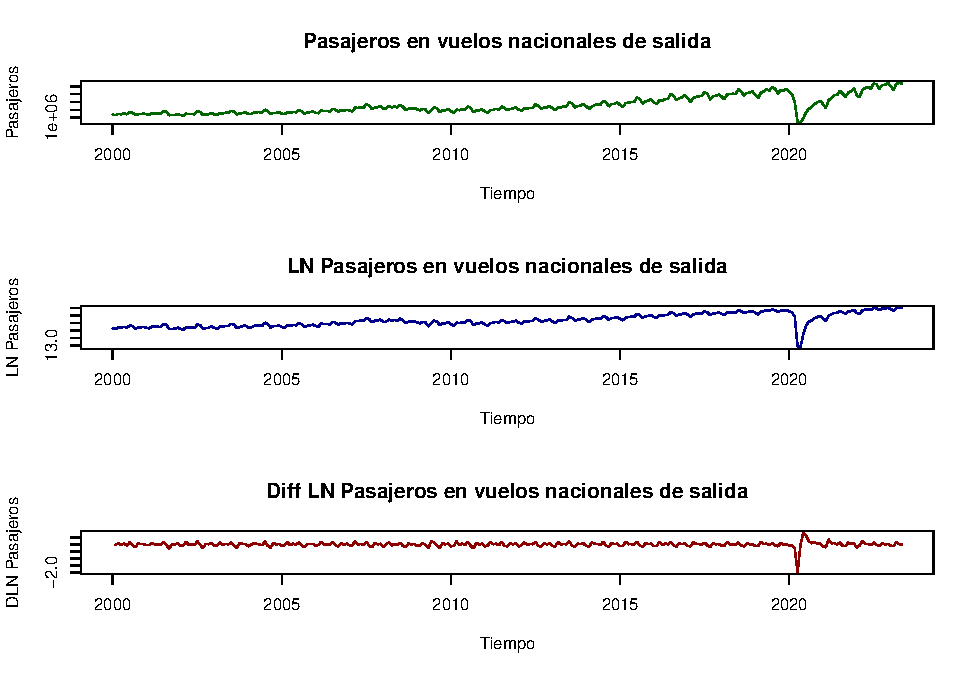
\includegraphics{Notas-Series-Tiempo_files/figure-latex/fig47-1} 

}

\caption{Pasajeros en vuelos de salidas nacionales en niveles y en diferencias logaritmicas}\label{fig:fig47}
\end{figure}

\begin{Shaded}
\begin{Highlighting}[]
\FunctionTok{par}\NormalTok{(}\AttributeTok{mfrow=}\FunctionTok{c}\NormalTok{(}\DecValTok{1}\NormalTok{,}\DecValTok{1}\NormalTok{))}
\end{Highlighting}
\end{Shaded}

A continuación, estimaremos un \(AR(2)\) para la serie en niveles bajo una transformación logarítmica (\(LPaxNal_t\)) y en diferencias logarítmitcas (\(DLPax_Nal_t\)). Para el primer caso obtenemos el siguiente resultado:

\begin{center}
\begin{tabular}{ c c c c c c } 
    $LPaxNal_t$ & $=$ & $14.6267$ & $+$ & $0.7637$  & $LPaxNal_{t-1}$ \\ 
    &  & $(0.1816)$ &  & $(0.0637)$ & \\
    &  &  & $+$ & $0.2025$ & $LPaxNal_{t-2}$ \\
    &  &  &  & $(0.0646)$ &
\end{tabular}
\end{center}

\begin{center}
\begin{tabular}{ c c c c c c c } 
    $\hat{\sigma}^2$ & $=$ & $0.01138$ & y & $AIC$ & $=$ & $-372.64$ 
\end{tabular}
\end{center}

Para el segundo caso obtenemos el siguiente resultado:

\begin{center}
\begin{tabular}{ c c c c c c } 
    $DLPaxNal_t$ & $=$ & $0.0050$ & $-$ & $0.3205$  & $DLPaxNal_{t-1}$ \\ 
    &  & $(0.0036)$ &  & $(0.0592)$ & \\
    &  &  & $-$ & $0.4242$ & $DLPaxNal_{t-2}$ \\
    &  &  &  & $(0.0591)$ &
\end{tabular}
\end{center}

\begin{center}
\begin{tabular}{ c c c c c c c } 
    $\hat{\sigma}^2$ & $=$ & $0.009378$ & y & $AIC$ & $=$ & $-418.3$ 
\end{tabular}
\end{center}

Para ambos casos entre parentésis indicamos los errores estándar y reportamos el estadístico de Akaike, AIC. Finalmente, podemos determinar si las soluciones serán convergentes, para ello en la Figura \ref{fig:fig48}\} mostramos las raíces asociadas a cada uno de los polinomios. De la inspección visual podemos concluir que ambas propuesta de AR(2) representan una solución convergente y estable.

\begin{Shaded}
\begin{Highlighting}[]
\FunctionTok{source}\NormalTok{(}\StringTok{"arroots.R"}\NormalTok{)}

\FunctionTok{source}\NormalTok{(}\StringTok{"plot.armaroots.R"}\NormalTok{)}

\NormalTok{AR\_LPax\_Nal }\OtherTok{\textless{}{-}} \FunctionTok{arima}\NormalTok{(LPax\_Nal, }\AttributeTok{order =} \FunctionTok{c}\NormalTok{(}\DecValTok{2}\NormalTok{, }\DecValTok{0}\NormalTok{, }\DecValTok{0}\NormalTok{), }\AttributeTok{method =} \StringTok{"ML"}\NormalTok{)}

\NormalTok{AR\_DLPax\_Nal }\OtherTok{\textless{}{-}} \FunctionTok{arima}\NormalTok{(DLPax\_Nal, }\AttributeTok{order =} \FunctionTok{c}\NormalTok{(}\DecValTok{2}\NormalTok{, }\DecValTok{0}\NormalTok{, }\DecValTok{0}\NormalTok{), }\AttributeTok{method =} \StringTok{"ML"}\NormalTok{)}

\FunctionTok{par}\NormalTok{(}\AttributeTok{mfrow=}\FunctionTok{c}\NormalTok{(}\DecValTok{1}\NormalTok{,}\DecValTok{2}\NormalTok{))}

\FunctionTok{plot.armaroots}\NormalTok{(}\FunctionTok{arroots}\NormalTok{(AR\_LPax\_Nal), }
               \AttributeTok{main=}\StringTok{"Inverse AR roots of }\SpecialCharTok{\textbackslash{}n}\StringTok{AR(2): LN Pax Nal"}\NormalTok{)}

\CommentTok{\#}
\FunctionTok{plot.armaroots}\NormalTok{(}\FunctionTok{arroots}\NormalTok{(AR\_DLPax\_Nal), }
               \AttributeTok{main=}\StringTok{"Inverse AR roots of }\SpecialCharTok{\textbackslash{}n}\StringTok{AR(2): Diff LN Pax Nal"}\NormalTok{)}
\end{Highlighting}
\end{Shaded}

\begin{figure}

{\centering 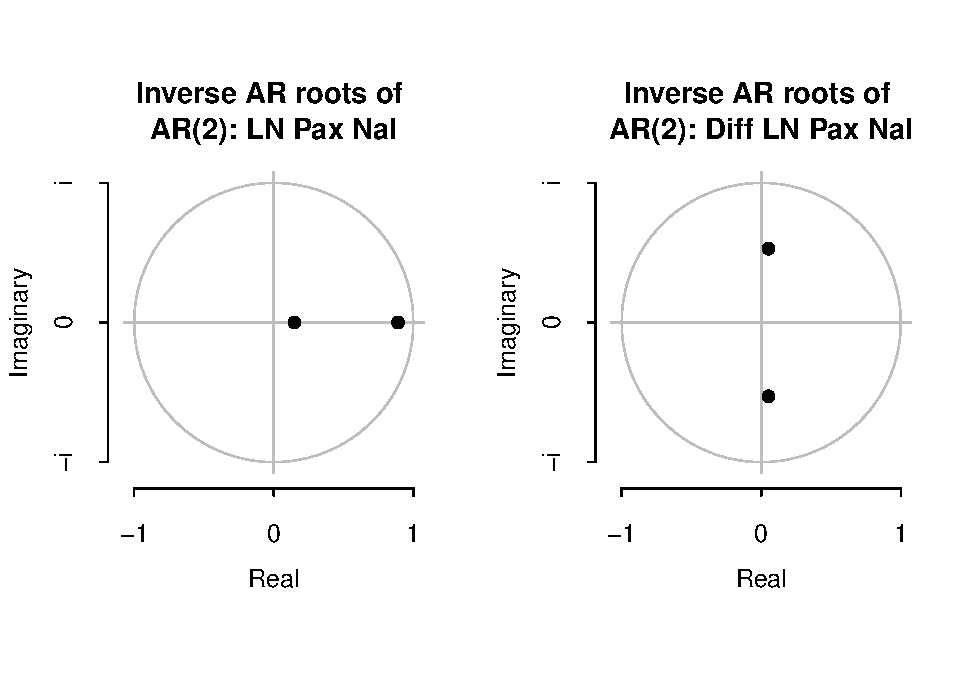
\includegraphics{Notas-Series-Tiempo_files/figure-latex/fig48-1} 

}

\caption{Inveso de las Raíces del polinomio característico}\label{fig:fig48}
\end{figure}

\begin{Shaded}
\begin{Highlighting}[]
\FunctionTok{par}\NormalTok{(}\AttributeTok{mfrow=}\FunctionTok{c}\NormalTok{(}\DecValTok{1}\NormalTok{,}\DecValTok{1}\NormalTok{))}
\end{Highlighting}
\end{Shaded}

\hypertarget{arp}{%
\subsection{AR(p)}\label{arp}}

Veremos ahora una generalización de los procesos autoregresivos (AR). Esta generalización es conocida como un proceso \(AR(p)\) y que puede ser descrito por la siguiente ecuación en diferencia estocástica:
\begin{equation}
    X_t = a_0 + a_1 X_{t-1} + a_2 X_{t-2} + a_3 X_{t-3} + \ldots + a_p X_{t-p} + U_t
    \label{ARp_Eq}
\end{equation}

Donde \(a_p \neq 0\), y \(U_t\) es un proceso puramente aleatorio con media cero (0), varianza constante (\(\sigma^2\)) y covarianza cero (0). Usando el operador rezago, \(L^k\), para \(k = 0, 1, 2, \ldots, p\), obtenemos la siguiente expresión de la ecuación (\ref{ARp_Eq}):
\begin{equation}
    (1 - a_1 L - a_2 L^2 - a_3 L^3 - \ldots - a_p L^p) X_t = a_0 + U_t
\end{equation}

Definamos el polinomio \(\alpha(L)\) como:
\begin{equation}
    \alpha(L) = 1 - a_1 L - a_2 L^2 - a_3 L^3 - \ldots - a_p L^p
    \label{Pol_A}
\end{equation}

De forma similar que en los procesos \(AR(1)\) y \(AR(2)\), las condiciones de estabilidad del proceso \(AR(p)\) estarán dadas por la solución de la ecuación característica:
\begin{equation}
    \lambda^p - a_1 \lambda^{p-1} - a_2 \lambda^{p-2} - a_3 \lambda^{p-3} - \ldots - a_p = 0
\end{equation}

Así, solo si el polinomio anterior tiene raíces cuyo valor absoluto sea menor a uno (\$ \textbar{}\lambda\_i\textbar{} \textless{} 1\$) y si \(1 - a_1 L - a_2 L^2 - a_3 L^3 - \ldots - a_p L^p < 1\) podremos decir que el proceso es convergente y estable. Lo anterior significa que la ecuación (\ref{Pol_A}) puede expresarse en términos de la descomposición de Wold o como la suma infinita de términos como:
\begin{equation}
    \frac{1}{1 - a_1 L  - a_2 L^2 - a_3 L^3  - \ldots - a_p L^p} = \psi_0 + \psi_1 L + \psi_2 L^2 + \psi_3 L^3 + \ldots
\end{equation}

Donde, por construcción de \(\alpha(L) \alpha^{-1}(L) = 1\) implica que \(\psi_0 = 1\). De forma similar a los proceso AR(1) y AR(2), es posible determinar el valor de los coefieentes \(\psi_j\) en términos de los coefientes \(a_i\). Así, la solución del proceso \(AR(p)\) estará dada por:
\begin{equation}
    X_t = \frac{a_0}{1 - a_1  - a_2 - a_3  - \ldots - a_p} + \sum^{\infty}_{j = 0} \psi_j U_{t-j}
    \label{ARp_Eq_Sol}
\end{equation}

Considerando la solución de la ecuación (\ref{ARp_Eq}) expresada en la ecuación (\ref{ARp_Eq_Sol}) podemos determinar los momentos del proceso y que estarán dados por una media como:
\begin{equation}
    \mathbb{E}[X_t] = \mu = \frac{a_o}{1 - a_1  - a_2 - a_3  - \ldots - a_p}
\end{equation}

Lo anterior, considerado que \(\mathbb{E}[U_t] = 0\), para todo \(t\). Para determinar la varianza del proceso, sin pérdida de generalidad, podemos definir una ecuación: \(\gamma(\tau) = \mathbb{E}[X_{t - \tau} X_t]\), la cual (omitiendo la constante, ya que la correlación de una constante con cuaquier variable aleatoria que depende del tiempo es cero (0)) puede ser escrita como:
\begin{equation}
    \gamma(\tau) = \mathbb{E}[(X_{t - \tau}) \cdot (a_1 X_{t-1} + a_2 X_{t-2} + a_3 X_{t-3} + \ldots + + a_p X_{t-p} + U_t)]
\end{equation}

Donde \(\tau = 0, 1, 2, \ldots, p\) y \(a_0 = 0\), lo que implica que \(\mu = 0\). De lo anterior obtenemos el siguiente conjunto de ecuaciones mediante sustituciones de los valores de \(\tau\):
\begin{eqnarray}
    \gamma(0) & = & a_1 \gamma(1) + a_2 \gamma(2) + \ldots + a_p \gamma(p) + \sigma^2 \nonumber \\
    \gamma(1) & = & a_1 \gamma(0) + a_2 \gamma(1) + \ldots + a_p \gamma(p-1) \nonumber \\
    \vdots \nonumber \\
    \gamma(p) & = & a_1 \gamma(p-1) + a_2 \gamma(p-2) + \ldots + a_p \gamma(0) \nonumber
\end{eqnarray}

De esta forma, es fácil observar que la ecuación general para \(p > 0\) estará dada por:
\begin{equation}
    \gamma(p) - a_1 \gamma(\tau - 1) - a_2 \gamma(\tau - 2) - \ldots - a_p \gamma(\tau - p) = 0
    \label{Gamma_p}
\end{equation}

Dividiendo la ecuación (\ref{Gamma_p}) por \(\gamma(0)\), se obtiene la siguiente ecuación:
\begin{equation}
    \rho(p) - a_1 \rho(\tau - 1) + a_2 \rho(\tau - 2) + \ldots + a_p \rho(\tau - p) = 0
\end{equation}

Así, podemos escribir el siguiente sistema de ecuaciones:
\begin{eqnarray}
    \rho(1) & = & a_1 + a_2 \rho(1) + a_3 \rho(2) + \ldots + a_p \rho(p-1) \nonumber \\
    \rho(2) & = & a_1 \rho(1) + a_2 + a_3 \rho(1) + \ldots + a_p \rho(p-2) \nonumber \\
    & \vdots & \nonumber \\
    \rho(p) & = & a_1 \rho(p-1) + a_2 \rho(p-2) + \ldots + a_p \nonumber
\end{eqnarray}

Lo anterior se puede expresar como un conjunto de vectores y matrices de la siguiente forma:
\begin{equation}
    \left[ 
    \begin{array}{c}
        \rho(1) \\
        \rho(2) \\
        \vdots \\
        \rho(p)
    \end{array} 
    \right]
    = 
    \left[ 
    \begin{array}{c c c c}
        1 & \rho(1) & \ldots & \rho(p - 1) \\
        \rho(1) & 1 & \ldots & \rho(p - 2) \\
        \rho(2) & \rho(1) & \ldots & \rho(p - 3) \\
        \vdots & \vdots & \ldots & \vdots \\
        \rho(p - 1) & \rho(p - 2) & \ldots & 1 \\
    \end{array} 
    \right]
    \left[ 
    \begin{array}{c}
        a_1 \\
        a_2 \\
        a_3 \\
        \vdots \\
        a_p \\
    \end{array} 
    \right]
\end{equation}

De lo anterior podemos escribir la siguiente ecuación que es una forma alternativa para expresar los valores de los coefientes \(a_i\) de la la solución del proceso \(AR(p)\):
\begin{equation}
    \mathbf{\rho} = \mathbf{R} \mathbf{a}
\end{equation}

Es decir, podemos obtener la siguiente expresión:
\begin{equation}
    \mathbf{a} = \mathbf{R}^{-1} \mathbf{\rho}
\end{equation}

Ahora veámos un ejemplo. Utilizaremos la serie de Pasajeros en vuelos internacionales de salida para estimar un \(AR(p)\) mediante el método de máxima verosimilitud (ML). Antes de realizar el proceso de estimación consideremos una transformación de la serie en logaritmos y una más en diferencias logaritmicas; lo anterior con el objeto de obtener un conjunto de series de tiempo suavizada y expresada en tasas de crecimiento, con un comportamiento parecido a un proceso estacionario.

Primero, para decidir si se realizará un \(AR(p)\) para la serie en niveles o en diferencias análizaremos su gráfica. La serie de e Pasajeros en vuelos internacionales de salidas se muestra en la Figura \ref{fig:fig49}\}. En está se muestra la gráfica de la serie en niveles (sin transformación logaritmica y con transformación logaritmica) y en diferencias logaritmicas mensuales (es decir, con diferencia respecto del mes inmediato anterior).

\begin{Shaded}
\begin{Highlighting}[]
\FunctionTok{library}\NormalTok{(ggplot2)}
\FunctionTok{library}\NormalTok{(dplyr)}
\FunctionTok{library}\NormalTok{(readxl)}
\FunctionTok{library}\NormalTok{(stats)}

\NormalTok{Datos }\OtherTok{\textless{}{-}} \FunctionTok{read\_excel}\NormalTok{(}\StringTok{"BD/Base\_Transporte.xlsx"}\NormalTok{, }\AttributeTok{sheet =} \StringTok{"Datos"}\NormalTok{, }\AttributeTok{col\_names =} \ConstantTok{TRUE}\NormalTok{)}

\CommentTok{\# En Niveles}
\NormalTok{Pax\_Int }\OtherTok{\textless{}{-}} \FunctionTok{ts}\NormalTok{(Datos}\SpecialCharTok{$}\NormalTok{Pax\_Int, }
              \AttributeTok{start =} \FunctionTok{c}\NormalTok{(}\DecValTok{2000}\NormalTok{, }\DecValTok{1}\NormalTok{), }
              \AttributeTok{freq =} \DecValTok{12}\NormalTok{)}

\CommentTok{\# Logaritmos:}
\NormalTok{LPax\_Int }\OtherTok{\textless{}{-}} \FunctionTok{ts}\NormalTok{(}\FunctionTok{log}\NormalTok{(Datos}\SpecialCharTok{$}\NormalTok{Pax\_Int), }
               \AttributeTok{start =} \FunctionTok{c}\NormalTok{(}\DecValTok{2000}\NormalTok{, }\DecValTok{1}\NormalTok{), }
               \AttributeTok{freq =} \DecValTok{12}\NormalTok{)}

\CommentTok{\# Diferencias mensuales:}
\NormalTok{DLPax\_Int }\OtherTok{\textless{}{-}} \FunctionTok{ts}\NormalTok{(}\FunctionTok{log}\NormalTok{(Datos}\SpecialCharTok{$}\NormalTok{Pax\_Int) }\SpecialCharTok{{-}} \FunctionTok{lag}\NormalTok{(}\FunctionTok{log}\NormalTok{(Datos}\SpecialCharTok{$}\NormalTok{Pax\_Int), }\DecValTok{1}\NormalTok{),}
                \AttributeTok{start =} \FunctionTok{c}\NormalTok{(}\DecValTok{2000}\NormalTok{, }\DecValTok{1}\NormalTok{), }
                \AttributeTok{freq =} \DecValTok{12}\NormalTok{)}

\CommentTok{\#}
\FunctionTok{par}\NormalTok{(}\AttributeTok{mfrow=}\FunctionTok{c}\NormalTok{(}\DecValTok{3}\NormalTok{,}\DecValTok{1}\NormalTok{))}

\FunctionTok{plot}\NormalTok{(Pax\_Int, }\AttributeTok{xlab =} \StringTok{"Tiempo"}\NormalTok{, }\AttributeTok{ylab =} \StringTok{"Pasajeros"}\NormalTok{,}
     \AttributeTok{main =} \StringTok{"Pasajeros en vuelos internacionales de salida"}\NormalTok{,}
     \AttributeTok{col =} \StringTok{"darkgreen"}\NormalTok{)}

\FunctionTok{plot}\NormalTok{(LPax\_Int, }\AttributeTok{xlab =} \StringTok{"Tiempo"}\NormalTok{, }\AttributeTok{ylab =} \StringTok{"LN Pasajeros"}\NormalTok{,}
     \AttributeTok{main =} \StringTok{"LN Pasajeros en vuelos internacionales de salida"}\NormalTok{,}
     \AttributeTok{col =} \StringTok{"darkblue"}\NormalTok{)}

\FunctionTok{plot}\NormalTok{(DLPax\_Int, }\AttributeTok{xlab =} \StringTok{"Tiempo"}\NormalTok{, }\AttributeTok{ylab =} \StringTok{"DLN Pasajeros"}\NormalTok{,}
     \AttributeTok{main =} \StringTok{"Diff LN Pasajeros en vuelos internacionales de salia"}\NormalTok{, }
     \AttributeTok{col =} \StringTok{"darkred"}\NormalTok{)}
\end{Highlighting}
\end{Shaded}

\begin{figure}

{\centering 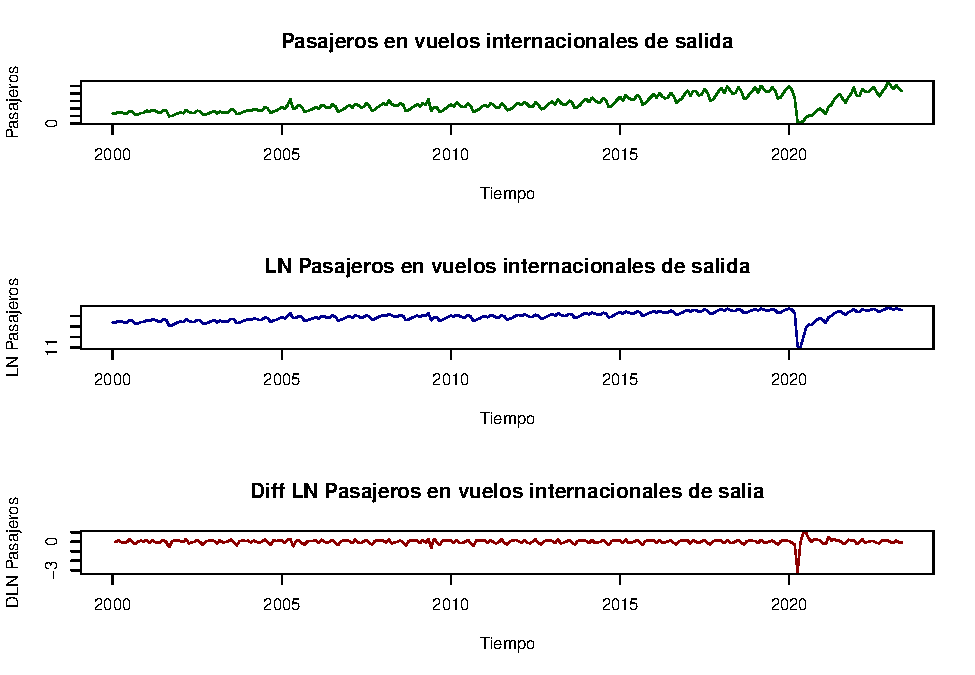
\includegraphics{Notas-Series-Tiempo_files/figure-latex/fig49-1} 

}

\caption{Pasajeros en vuelos internacionales de salida en niveles y en diferencias logaritmicas}\label{fig:fig49}
\end{figure}

\begin{Shaded}
\begin{Highlighting}[]
\FunctionTok{par}\NormalTok{(}\AttributeTok{mfrow=}\FunctionTok{c}\NormalTok{(}\DecValTok{1}\NormalTok{,}\DecValTok{1}\NormalTok{))}
\end{Highlighting}
\end{Shaded}

De la gráfica en la Figura \ref{fig:fig49}\} observamos que quizá le mejor forma de estimar un AR(p) es mediante la serie en diferencias, ya que ésta es la que parece ser una serie estacionaria. A continuación, estimaremos una AR(4) para la serie en diferencias logarimitcas (\(DLPaxInt_t\)):

\begin{center}
\begin{tabular}{ c c c c c c } 
    $DLPaxInt_t$ & $=$ & $0.0050$ & $-$ & $0.2701$  & $DLPaxInt_{t-1}$ \\ 
    &  & $(0.0052)$ &  & $(0.0655)$ & \\
    &  &  & $-$ & $0.4326$ & $DLPaxNal_{t-2}$ \\
    &  &  &  & $(0.0664)$ & \\
    &  &  & $-$ & $0.1956$ & $DLPaxNal_{t-3}$ \\
    &  &  &  & $(0.0664)$ & \\
    &  &  & $-$ & $0.0316$ & $DLPaxNal_{t-4}$ \\
    &  &  &  & $(0.0653)$ & 
\end{tabular}
\end{center}

\begin{center}
\begin{tabular}{ c c c c c c c } 
    $\hat{\sigma}^2$ & $=$ & $0.02371$ & y & $AIC$ & $=$ & $-198.16$ 
\end{tabular}
\end{center}

Entre parentésis indicamos los errores estándar y reportamos el estadístico de Akaike, AIC. Finalmente, podemos determinar si las soluciones serán convergentes, para ello en la Figura \ref{fig:fig410}\} mostramos las raíces asociadas a cada uno de los polinomios. De la inspección visual podemos concluir que el AR(4) representan una solución convergente y estable.

\begin{Shaded}
\begin{Highlighting}[]
\FunctionTok{source}\NormalTok{(}\StringTok{"arroots.R"}\NormalTok{)}

\FunctionTok{source}\NormalTok{(}\StringTok{"plot.armaroots.R"}\NormalTok{)}

\NormalTok{AR\_LPax\_Int }\OtherTok{\textless{}{-}} \FunctionTok{arima}\NormalTok{(LPax\_Int, }\AttributeTok{order =} \FunctionTok{c}\NormalTok{(}\DecValTok{4}\NormalTok{, }\DecValTok{0}\NormalTok{, }\DecValTok{0}\NormalTok{), }\AttributeTok{method =} \StringTok{"ML"}\NormalTok{)}

\NormalTok{AR\_DLPax\_Int }\OtherTok{\textless{}{-}} \FunctionTok{arima}\NormalTok{(DLPax\_Int, }\AttributeTok{order =} \FunctionTok{c}\NormalTok{(}\DecValTok{4}\NormalTok{, }\DecValTok{0}\NormalTok{, }\DecValTok{0}\NormalTok{), }\AttributeTok{method =} \StringTok{"ML"}\NormalTok{)}

\FunctionTok{par}\NormalTok{(}\AttributeTok{mfrow=}\FunctionTok{c}\NormalTok{(}\DecValTok{1}\NormalTok{,}\DecValTok{2}\NormalTok{))}

\FunctionTok{plot.armaroots}\NormalTok{(}\FunctionTok{arroots}\NormalTok{(AR\_LPax\_Nal), }
               \AttributeTok{main=}\StringTok{"Inverse AR roots of }\SpecialCharTok{\textbackslash{}n}\StringTok{AR(2): LN Pax Int"}\NormalTok{)}

\CommentTok{\#}
\FunctionTok{plot.armaroots}\NormalTok{(}\FunctionTok{arroots}\NormalTok{(AR\_DLPax\_Nal), }
               \AttributeTok{main=}\StringTok{"Inverse AR roots of }\SpecialCharTok{\textbackslash{}n}\StringTok{AR(2): Diff LN Pax Int"}\NormalTok{)}
\end{Highlighting}
\end{Shaded}

\begin{figure}

{\centering 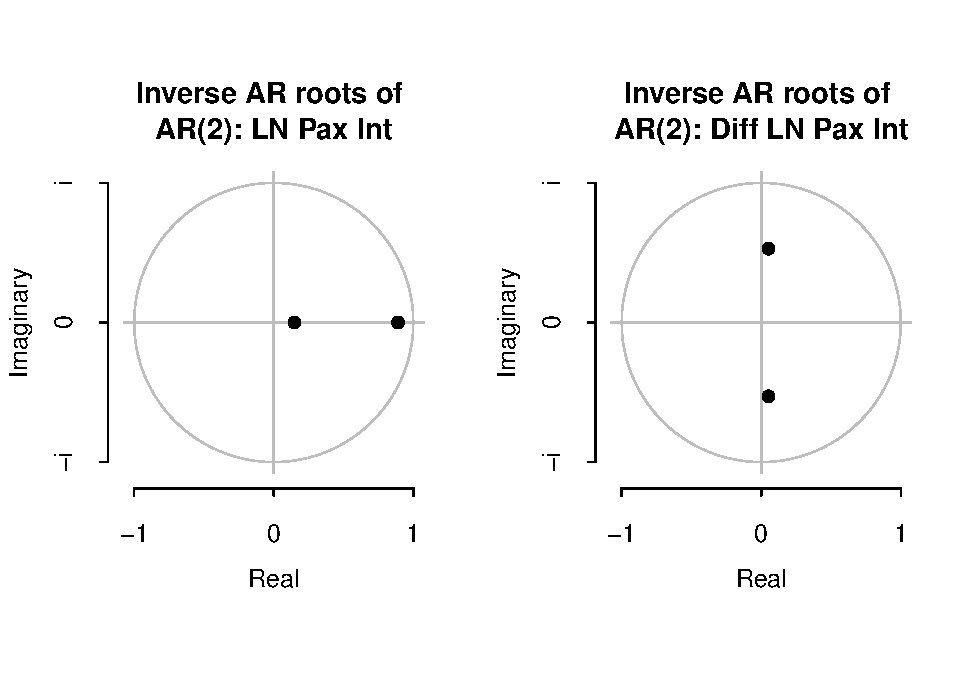
\includegraphics{Notas-Series-Tiempo_files/figure-latex/fig410-1} 

}

\caption{Inveso de las Raíces del polinomio característico}\label{fig:fig410}
\end{figure}

\begin{Shaded}
\begin{Highlighting}[]
\FunctionTok{par}\NormalTok{(}\AttributeTok{mfrow=}\FunctionTok{c}\NormalTok{(}\DecValTok{1}\NormalTok{,}\DecValTok{1}\NormalTok{))}
\end{Highlighting}
\end{Shaded}

\hypertarget{procesos-de-medias-muxf3viles-ma}{%
\section{Procesos de Medias Móviles (MA)}\label{procesos-de-medias-muxf3viles-ma}}

\hypertarget{ma1}{%
\subsection{MA(1)}\label{ma1}}

Una vez planteado el proceso generalizado de \(AR(p)\), iniciamos el planteamiento de los proceso de medias móviles, denotados como \(MA(q)\). Iniciemos con el planteamiento del proceso \(MA(1)\), que se puede escribir como una ecuación como la siguiente:
\begin{equation}
    X_t = \mu + U_t - b_1 U_{t-1}
    \label{MA1_Eq}
\end{equation}

O como:
\begin{equation}
    X_t - \mu = (1 - b_1 L) U_{t}
\end{equation}

Donde \(U_t\) es un proceso puramente aleatorio, es decir, con \(\mathbb{E}[U_t] = 0\), \(Var[U_t] = \sigma^2\), y \(Cov[U_t, U_s] = 0\). Así, un proceso \(MA(1)\) puede verse como un proceso AR con una descomposición de Wold en la que \(\psi_0 = 1\), \(\psi_1 = - b_1\) y \(\psi_j = 0\) para todo \(j > 1\).

Al igual que los procesos autoregresivos, determinaremos los momentos de un proceso \(MA(1)\). En el caso de la media observamos que será:
\begin{eqnarray}
    \mathbb{E}[X_t] & = & \mu + \mathbb{E}[U_t] - b_1 \mathbb{E}[U_{t - 1}] \nonumber \\
    & = & \mu
\end{eqnarray}

Por su parte la varianza estará dada por:
\begin{eqnarray}
    Var[X_t] & = & \mathbb{E}[(X_t - \mu)^2] \nonumber \\
    & = & \mathbb{E}[(U_t - b_1 U_{t-1})^2] \nonumber \\
    & = & \mathbb{E}[U_t^2 - 2 b_1 U_t U_{t-1} + b_1^2 U_{t - 1}^2] \nonumber \\
    & = &\mathbb{E}[U_t^2] - 2 b_1 \mathbb{E}[U_t U_{t-1}] + b_1^2 \mathbb{E}[U_{t - 1}^2]] \nonumber \\
    & = & \sigma^2 + b_1^2 \sigma^2 \nonumber \\
    & = & (1 + b_1^2) \sigma^2 = \gamma(0)
\end{eqnarray}

De esta forma, la varianza del proceso es constante en cualquier periodo \(t\). Para determinar la covarianza utilizaremos la siguiente ecuación:
\begin{eqnarray}
    \mathbb{E}[(x_t - \mu)(x_{t + \tau} - \mu)] & = & \mathbb{E}[(U_t - b_1 U_{t-1})(U_{t + \tau} - b_1 U_{t + \tau - 1})] \nonumber \\
    & = & \mathbb{E}[U_t U_{t + \tau} - b_1 U_t U_{t + \tau - 1} - b_1 U_{t - 1} U_{t + \tau} \nonumber \\
    &   & + b_1^2 U_{t - 1} U_{t + \tau - 1}] \nonumber \\
    & = & \mathbb{E}[U_t U_{t + \tau}] - b_1 \mathbb{E}[U_t U_{t + \tau - 1}] \nonumber \\
    &   & - b_1 \mathbb{E}[U_{t - 1} U_{t + \tau}] + b_1^2 \mathbb{E}[U_{t - 1} U_{t + \tau - 1}]
    \label{MA1_Cov}
\end{eqnarray}

Si hacemos sustituciones de diferentes valores de \(\tau\) en la ecuación (\ref{MA1_Cov}) notaremos que la covarianza será distinta de cero únicamente para el caso de \(\tau = 1, -1\). En ambos casos tendremos como resultado:
\begin{eqnarray}
    \mathbb{E}[(x_t - \mu)(x_{t + 1} - \mu)] & = & \mathbb{E}[(x_t - \mu)(x_{t - 1} - \mu)] \nonumber \\
    & = & - b_1 \mathbb{E}[U_t U_{t}] \nonumber \\
    & = & - b_1 \mathbb{E}[U_{t - 1} U_{t - 1}] \nonumber \\ 
    & = & - b_1^2 \sigma^2 = \gamma(1)
\end{eqnarray}

De esta forma tendremos que las funciones de autocorrelación estarán dadas por los siguientes casos:
\begin{eqnarray}
    \rho(0) & = & 1 \nonumber \\
    \rho(1) & = & \frac{- b_1}{1 + b_1^2} \nonumber \\
    \rho(\tau) & = & 0 \text{ para todo } \tau > 1 \nonumber 
\end{eqnarray}

Ahora regresando a la ecuación (\ref{MA1_Eq}), su solución la podemos expresar como:
\begin{eqnarray}
    U_ t & = & - \frac{\mu}{1 - b_1} + \frac{1}{1 - b_1 L} X_t \nonumber \\
    & = & - \frac{\mu}{1 - b_1} + X_t + b_1 X_{t-1} + b_1^2 X_{t-2} + \ldots \nonumber
\end{eqnarray}

Donde la condición para que se cumpla esta ecuación es que \$ \textbar b\_1\textbar{} \textless{} 1\$. La manera de interpretar esta condición es como una condición de estabilidad de la solución y cómo una condición de invertibilidad. Notemos que un \(MA(1)\) (y en general un \(MA(q)\)) es equivalente a un \(AR(\infty)\), es decir, cuando se invierte un MA se genera un AR con infinitos rezagos.

En esta sección no desarrollaremos un ejemplo, primero explicaremos en qué consiste una modelación del tipo \(MA(q)\) y después platearemos un ejemplo en concreto.

\hypertarget{maq}{%
\subsection{MA(q)}\label{maq}}

En general, el proceso de medias móviles de orden \(q\), \(MA(q)\), puede ser escrito como:
\begin{equation}
    X_t = \mu + U_t - b_1 U_{t-1} - b_2 U_{t-2} - \ldots - b_q U_{t-q}
    \label{MAq_EQ}
\end{equation}

Podemos reescribir la ecuación (\ref{MAq_EQ}) utilizando el operador rezago, así tendrémos el proceso de \(MA(q)\) como:
\begin{eqnarray}
    X_t - \mu & = & (1 - b_1 L - b_2 L^2 - \ldots - b_q L^q) U_{t} \nonumber \\
    X_t - \mu & = & \beta(L) U_t
    \label{MAq_Red}
\end{eqnarray}

Donde \(U_t\) es un proceso puramente aleatorio con \(\mathbb{E}[U_t] = 0\), \(Var[U_t] = \mathbb{E}[U_t^2] = 0\) y \(Cov[U_t, U_s] = \mathbb{E}[U_t, U_s] = 0\), y \(\beta(L) = 1 - b_1 L - b_2 L^2 - \ldots - b_q L^q\) es un polinomio del operador rezago \(L\). la ecuación (\ref{MAq_Red}) puede ser interpretada como un proceso \(AR(q)\) sobre la serie \(U_t\).

Ahora determinemos los momentos de un proceso \(MA(q)\):
\begin{eqnarray}
    \mathbb{E}[X_t] & = & \mathbb{E}[\mu + U_t - b_1 U_{t-1} - b_2 U_{t-2} - \ldots - b_q U_{t-q}] \nonumber \\
    & = & \mu + \mathbb{E}[U_t] - b_1 \mathbb{E}[U_{t-1}] - b_2 \mathbb{E}[U_{t-2}] - \ldots - b_q \mathbb{E}[U_{t-q}] \nonumber \\
    & = & \mu
\end{eqnarray}

En el caso de la varianza tenemos que se puede expresar como:
\begin{eqnarray}
    Var[X_t] & = & \mathbb{E}[(X_t - \mu)^2] \nonumber \\
    & = & \mathbb{E}[(U_t - b_1 U_{t-1} - b_2 U_{t-2} - \ldots - b_q U_{t-q})^2] \nonumber \\
    & = & \mathbb{E}[U_t^2 + b_1^2 U_{t-1}^2 + b_2^2 U_{t-2}^2 + \ldots + b_q^2 U_{t-q}^2 \nonumber \\
    &   & - 2 b_1 U_t U_{t - 1} - \ldots - 2 b_{q - 1} b_q U_{t - q + 1} U_{t - q}] \nonumber \\
    & = & \mathbb{E}[U_t^2] + b_1^2 \mathbb{E}[U_{t-1}^2] + b_2^2 \mathbb{E}[U_{t-2}^2] + \ldots + b_q^2 \mathbb{E}[U_{t-q}^2] \nonumber \\
    &   & - 2 b_1 \mathbb{E}[U_t U_{t - 1}] - \ldots - 2 b_{q - 1} b_q \mathbb{E}[U_{t - q + 1} U_{t - q}] \nonumber \\
    & = & \sigma^2 + b^2_1 \sigma^2 + b^2_2 \sigma^2 + \ldots + b^2_q \sigma^2 \nonumber \\
    & = & (1 + b^2_1 + b^2_2 + \ldots + b^2_q) \sigma^2
\end{eqnarray}

En el caso de las covarianzas podemos utilizar una idea similar al caso del \(AR(p)\), construir una expresión general para cualquier rezago \(\tau\):
\begin{eqnarray}
    Cov[X_t, X_{t + \tau}] & = & \mathbb{E}[(X_t - \mu)(X_{t + \tau} - \mu)] \nonumber \\
    & = & \mathbb{E}[(U_t - b_1 U_{t-1} - b_2 U_{t-2} - \ldots - b_q U_{t-q}) \nonumber \\
    &   & (U_{t + \tau} - b_1 U_{t + \tau -1} - b_2 U_{t + \tau -2} - \ldots - b_q U_{t + \tau - q})] \nonumber
\end{eqnarray}

La expresión anterior se puede desarrollar para múltiples casos de \(\tau = 1, 2, \ldots, q\). De esta forma tenemos el siguiente sistema:
\begin{eqnarray}
    \tau = 1 & : & \gamma(1) = (- b_1 + b_1 b_2 + \ldots + b_{q-1} b_q) \sigma^2 \nonumber \\
    \tau = 2 & : & \gamma(2) = (- b_2 + b_1 b_3 + \ldots + b_{q-2} b_q) \sigma^2 \nonumber \\
    & \vdots & \nonumber \\
    \tau = q & : & \gamma(q) = b_q \sigma^2 \nonumber
\end{eqnarray}

Donde \(\gamma(\tau) = 0\) para todo \(\tau > q\). Es decir, todas las autocovarianzas y autocorrelaciones con ordenes superiores a \(q\) son cero (0). De esta forma, esta caracterítica teórica permite identificar el orden de \(MA(q)\) visualizando la función de autocorrelación y verificando a partir de cual valor de rezago la autocorrelación es no significaiva.

Regresando al problema original que es el de determinar una solución para la eucación (\ref{MAq_EQ}), tenemos que dicha solución estará dada por un \(AR(\infty)\) en términos de \(U_t\):
\begin{eqnarray}
    U_t & = & - \frac{\mu}{1 - b_1 - b_2 - \ldots - b_q} + \beta(L)^{-1} X_t \nonumber \\
    &   & - \frac{\mu}{1 - b_1 - b_2 - \ldots - b_q} + \sum_{j = 0}^{\infty} c_j X_{t-j} 
    \label{MAq_Eq_Sol}
\end{eqnarray}

Donde se cumple que: \(1 = (1 - b_1 L^1 - b_2 L^2 - \ldots - b_q L^q)(1 - c_1 L - c_2 L^2 - \ldots)\) y los coeficientes \(c_j\) se pueden determinar por un método de coeficientes indeterminados y en términos de los valores \(b_i\). De igual forma que en el caso de la ecuación (\ref{ARp_Eq}), en la ecuación (\ref{MAq_Eq_Sol}) se deben cumplir condiciones de estabilidad asociadas con las raíces del polinomio carácterististico dado por:
\begin{equation}
    1 - b_1 x - b_2 x^2 - \ldots b_q x^q = 0
\end{equation}

El cual debe cumplir que \$ \textbar x\_i\textbar{} \textless{} 1\$ y que \(1 - b_1 - b_2 - \ldots b_q < 1\).

Ahora veamos un ejemplo del proceso \(MA(q)\), para lo cual retomaremos la serie de Pasajeros transportados en el metro de la CDMX (\(PaxMetro\)). Estimaremos el \(MA(q)\) mediante el método de máxima verosimilitud (ML). Antes de realizar el proceso de estimación consideremos una transformación de la serie en logaritmos y una más en diferencias logaritmicas; lo anterior con el objeto de obtener un conjunto de series de tiempo suavizada y expresada en tasas de crecimiento, con un comportamiento parecido a un proceso estacionario.

La serie de Pasajeros transportados en el metro de la CDMX se muestra en la Figura \ref{fig:fig46}\} se muestra la gráfica de la serie en niveles (sin transformación logarítmica y con transformación logarítmica) y en diferencias logarítmicas mensuales (es decir, con una diferencia respecto del mes inmediato anterior). Utilizaremos la serie en diferencias, ya que es la que parece ser estacionaria. Esta serie tiene la peculiaridad de que tiene un salto a la baja y uno al alza entre septiembre de 2017 y octubre de 2017. Para controlar ese efecto, en nuestro modelo \(MA(q)\) incluiremos dos variables dummies para dichos meses.

A continuación, estimaremos una \(MA(4)\) para la serie en diferencias:

\begin{center}
\begin{tabular}{ c c c c c c } 
    $DLPaxMetro_t$ & $=$ & $0.0000$ & $-$ & $0.7804$  & $U_{t-1}$ \\ 
    &  & $(0.0000)$ &  & $(0.0661)$ & \\
    &  &  & $+$ & $0.3591$ & $U_{t-2}$ \\
    &  &  &  & $(0.0826)$ & \\
    &  &  & $-$ & $0.2775$ & $U_{t-3}$ \\
    &  &  &  & $(0.0908)$ & \\
    &  &  & $-$ & $0.1120$ & $U_{t-4}$ \\
    &  &  &  & $(0.0769)$ & \\
    &  &  & $-$ & $0.3789$ & $DSep2017$ \\
    &  &  &  & $(0.0436)$ & \\
    &  &  & $+$ & $0.3695$ & $DOct2017$ \\
    &  &  &  & $(0.0434)$ & 
\end{tabular}
\end{center}

\begin{center}
\begin{tabular}{ c c c c c c c } 
    $\hat{\sigma}^2$ & $=$ & $0.002176$ & y & $AIC$ & $=$ & $-749.94$ 
\end{tabular}
\end{center}

Entre parentésis indicamos los errores estándar y al final reportamos el estadístico de Akaike, AIC. Finalmente, podemos determinar si la solución serán convergente, para ello en la Figura \ref{fig:fig411}\} mostramos las raíces asociadas a cada uno de los polinomios. De la inspección visual podemos concluir que ambas propuesta de AR(2) representan una solución convergente y estable.

\begin{Shaded}
\begin{Highlighting}[]
\FunctionTok{library}\NormalTok{(ggplot2)}
\FunctionTok{library}\NormalTok{(dplyr)}
\FunctionTok{library}\NormalTok{(readxl)}
\FunctionTok{library}\NormalTok{(stats)}

\NormalTok{Datos }\OtherTok{\textless{}{-}} \FunctionTok{read\_excel}\NormalTok{(}\StringTok{"BD/Base\_Transporte\_ARIMA.xlsx"}\NormalTok{, }\AttributeTok{sheet =} \StringTok{"Datos"}\NormalTok{, }\AttributeTok{col\_names =} \ConstantTok{TRUE}\NormalTok{)}

\FunctionTok{source}\NormalTok{(}\StringTok{"maroots.R"}\NormalTok{)}

\FunctionTok{source}\NormalTok{(}\StringTok{"plot.armaroots.R"}\NormalTok{)}

\NormalTok{Pax\_Metro }\OtherTok{\textless{}{-}} \FunctionTok{ts}\NormalTok{(Datos}\SpecialCharTok{$}\NormalTok{Pax\_Metro, }
                \AttributeTok{start =} \FunctionTok{c}\NormalTok{(}\DecValTok{2000}\NormalTok{, }\DecValTok{1}\NormalTok{), }
                \AttributeTok{freq =} \DecValTok{12}\NormalTok{)}

\NormalTok{LPax\_Metro }\OtherTok{\textless{}{-}} \FunctionTok{ts}\NormalTok{(}\FunctionTok{log}\NormalTok{(Datos}\SpecialCharTok{$}\NormalTok{Pax\_Metro), }
                 \AttributeTok{start =} \FunctionTok{c}\NormalTok{(}\DecValTok{2000}\NormalTok{, }\DecValTok{1}\NormalTok{), }
                 \AttributeTok{freq =} \DecValTok{12}\NormalTok{)}

\NormalTok{DLPax\_Metro }\OtherTok{\textless{}{-}} \FunctionTok{ts}\NormalTok{(}\FunctionTok{log}\NormalTok{(Datos}\SpecialCharTok{$}\NormalTok{Pax\_Metro) }\SpecialCharTok{{-}} \FunctionTok{lag}\NormalTok{(}\FunctionTok{log}\NormalTok{(Datos}\SpecialCharTok{$}\NormalTok{Pax\_Metro), }\DecValTok{1}\NormalTok{),}
                  \AttributeTok{start =} \FunctionTok{c}\NormalTok{(}\DecValTok{2000}\NormalTok{, }\DecValTok{1}\NormalTok{), }
                  \AttributeTok{freq =} \DecValTok{12}\NormalTok{)}

\NormalTok{D\_Sep2017 }\OtherTok{\textless{}{-}} \FunctionTok{ts}\NormalTok{(Datos}\SpecialCharTok{$}\NormalTok{D\_Sep2017, }
                \AttributeTok{start =} \FunctionTok{c}\NormalTok{(}\DecValTok{2000}\NormalTok{, }\DecValTok{1}\NormalTok{), }
                \AttributeTok{freq =} \DecValTok{12}\NormalTok{)}

\NormalTok{D\_Abr2020 }\OtherTok{\textless{}{-}} \FunctionTok{ts}\NormalTok{(Datos}\SpecialCharTok{$}\NormalTok{D\_Abr2020, }
                \AttributeTok{start =} \FunctionTok{c}\NormalTok{(}\DecValTok{2000}\NormalTok{, }\DecValTok{1}\NormalTok{), }
                \AttributeTok{freq =} \DecValTok{12}\NormalTok{)}

\NormalTok{D\_May2020   }\OtherTok{\textless{}{-}} \FunctionTok{ts}\NormalTok{(Datos}\SpecialCharTok{$}\NormalTok{D\_May2020, }
                \AttributeTok{start =} \FunctionTok{c}\NormalTok{(}\DecValTok{2000}\NormalTok{, }\DecValTok{1}\NormalTok{), }
                \AttributeTok{freq =} \DecValTok{12}\NormalTok{)}

\NormalTok{MA\_LPax\_Metro }\OtherTok{\textless{}{-}} \FunctionTok{arima}\NormalTok{(LPax\_Metro, }\AttributeTok{order =} \FunctionTok{c}\NormalTok{(}\DecValTok{0}\NormalTok{, }\DecValTok{0}\NormalTok{, }\DecValTok{4}\NormalTok{), }
                       \AttributeTok{method =} \StringTok{"ML"}\NormalTok{)}

\NormalTok{MA\_LPax\_Metro\_2 }\OtherTok{\textless{}{-}} \FunctionTok{arima}\NormalTok{(LPax\_Metro, }\AttributeTok{order =} \FunctionTok{c}\NormalTok{(}\DecValTok{0}\NormalTok{, }\DecValTok{0}\NormalTok{, }\DecValTok{4}\NormalTok{),}
                       \AttributeTok{xreg =} \FunctionTok{cbind}\NormalTok{(D\_Abr2020, D\_Sep2017, D\_May2020),}
                       \AttributeTok{method =} \StringTok{"ML"}\NormalTok{)}

\FunctionTok{par}\NormalTok{(}\AttributeTok{mfrow=}\FunctionTok{c}\NormalTok{(}\DecValTok{1}\NormalTok{,}\DecValTok{2}\NormalTok{))}

\FunctionTok{plot.armaroots}\NormalTok{(}\FunctionTok{maroots}\NormalTok{(MA\_LPax\_Metro), }
               \AttributeTok{main=}\StringTok{"Inverse MA roots of }\SpecialCharTok{\textbackslash{}n}\StringTok{MA(p): LN PAx Metro"}\NormalTok{)}

\FunctionTok{plot.armaroots}\NormalTok{(}\FunctionTok{maroots}\NormalTok{(MA\_LPax\_Metro\_2), }
               \AttributeTok{main=}\StringTok{"Inverse MA roots of }\SpecialCharTok{\textbackslash{}n}\StringTok{MA(p): LN PAx Metro con Dummy"}\NormalTok{)}
\end{Highlighting}
\end{Shaded}

\begin{figure}

{\centering 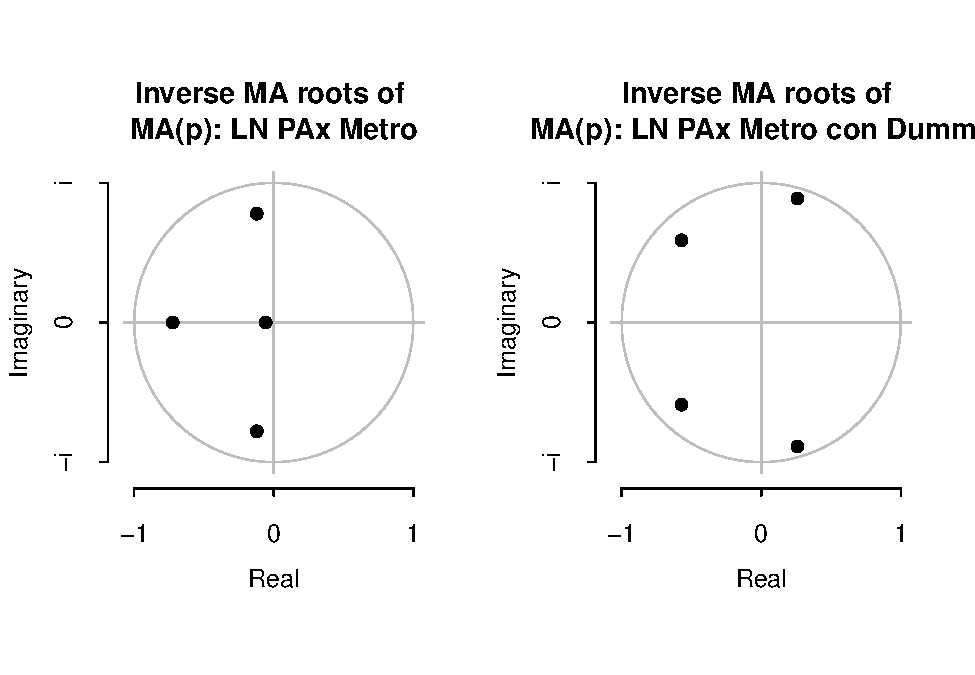
\includegraphics{Notas-Series-Tiempo_files/figure-latex/fig411-1} 

}

\caption{Inveso de las Raíces del polinomio característico}\label{fig:fig411}
\end{figure}

\begin{Shaded}
\begin{Highlighting}[]
\FunctionTok{par}\NormalTok{(}\AttributeTok{mfrow=}\FunctionTok{c}\NormalTok{(}\DecValTok{1}\NormalTok{,}\DecValTok{1}\NormalTok{))}
\end{Highlighting}
\end{Shaded}

\hypertarget{procesos-armap-q-y-arimap-d-q}{%
\section{Procesos ARMA(p, q) y ARIMA(p, d, q)}\label{procesos-armap-q-y-arimap-d-q}}

Hemos establecido algunas relaciones las de los porcesos AR y los procesos MA, es decir, cómo un \(MA(q)\) de la serie \(X_t\) puede ser reexpresada como un \(AR(\infty)\) de la serie \(U_t\), y viceversa un \(AR(p)\) de la serie \(X_t\) puede ser reeexpresada como un \(MA(\infty)\).

En este sentido, para cerrar esta sección veámos el caso de la especificación que conjunta ambos modelos en un modelo general conocido como \(ARMA(p, q)\) o \(ARIMA(p, d, q)\). La diferencia entre el primero y el segundo es las veces que su tuvo que diferenciar la serie analizada, registro que se lleva en el índice \(d\) de los paramétros dentro del concepto \(ARIMA(p, d, q)\). No obstante, en general nos referiremos al modelo como \(ARMA(p, q)\) y dependerá del analista si modela la serie en niveles (por ejemplo, en logaritmos) o en diferencias logarítmicas (o diferencias sin logaritmos).

\hypertarget{arma1-1}{%
\subsection{ARMA(1, 1)}\label{arma1-1}}

Dicho lo anterior vamos a empezar con el análisis de un \(ARMA(1, 1)\). Un proceso \(ARMA(1, 1)\) puede verse como:
\begin{equation}
    X_t = \delta + a_1 X_{t - 1} + U_t - b_1 U_{t - 1}
    \label{ARMA11_Eq}
\end{equation}

Aplicando el operado rezago podemos rescribir la ecuación (\ref{ARMA11_Eq}) como:
\begin{equation}
    (1 - a_1 L) X_t = \delta + (1 - b_1 L) U_t
\end{equation}

Donde \(U_t\) es un proceso pueramente aleatorio como en los casos de \(AR(p)\) y \(MA(q)\), y \(X_t\) puede ser una serie en niveles o en diferencias (ambas, en términos logarítmicos).

Así, el modelo \(ARIMA (p, q)\) también tiene una representación de Wold que estará dada por las siguientes expresiones:
\begin{equation}
    X_t = \frac{\delta}{1 - a_1} + \frac{1 - b_1 L}{1 - a_1 L} U_t
    \label{ARMA11_Prev}
\end{equation}

Donde \(a_1 \neq b_1\), puesto que en caso contrario \(X_t\) sería un proceso puramente aleatorio con una media \(\mu = \frac{\delta}{1 - a_1}\). Así, podemos reescribir la descomposición de Wold a partir del componente de la ecuación (\ref{ARMA11_Prev}):
\begin{equation}
    \frac{1 - b_1 L}{1 - a_1 L} = \psi_0 + \psi_1 L + \psi_2 L^2 + \psi_3 L^3 + \ldots 
    \label{ARMA11_EQ_Wold}
\end{equation}

Está ecuación es equivalente a la expresión:
\begin{eqnarray}
    (1 - b_1 L) & = & (1 - a_1 L)(\psi_0 + \psi_1 L + \psi_2 L^2 + \psi_3 L^3 + \ldots) \nonumber \\
    & = & \psi_0 + \psi_1 L + \psi_2 L^2 + \psi_3 L^3 + \ldots \nonumber \\
    &   & - a_1 \psi_0 L - a_1 \psi_1 L^2 - a_2 \psi_2 L^3 - a_1 \psi_3 L^4 - \ldots \nonumber
\end{eqnarray}

De esta forma podemos establecer el siguiente sistema de coeficientes indeterminados:

\begin{center}
\begin{tabular}{ c c c c } 
    $L^0 :$ & $ $ & $\Rightarrow$ & $\psi_0 = 1$ \\
    $L^1 :$ & $\psi_1 - a_1 \psi_0 = - b_1$ & $\Rightarrow$ & $\psi_1 = a_1 - b_1$ \\
    $L^2 :$ & $\psi_2 - a_1 \psi_1 = 0$ & $\Rightarrow$ & $\psi_2 = a_1(a_1 - b_1)$ \\
    $L^3 :$ & $\psi_3 - a_1 \psi_2 = 0$ & $\Rightarrow$ & $\psi_3 = a^2_1(a_1 - b_1)$ \\
    $\vdots$ & $\vdots$ & $\vdots$ & $\vdots$ \\
    $L^j :$ & $\psi_j - a_1 \psi_{j - 1} = 0$ & $\Rightarrow$ & $\psi_j = a^{j - 1}_1(a_1 - b_1)$
\end{tabular}
\end{center}

Así, la solución a la ecuación (\ref{ARMA11_Eq}) estará dada por la siguiente generalización:
\begin{equation}
    X_t = \frac{\delta}{1 - a_1} + U_t + (a_1 - b_1) U_{t - 1} + a_1(a_1 - b_1) U_{t - 2} + a_1^2(a_1 - b_1) U_{t - 3} + \ldots
    \label{ARMA11_Sol}
\end{equation}

En la ecuación (\ref{ARMA11_Sol}) las condiciones de estabilidad y de invertibilidad del sistema (de un MA a un AR, y viceversa) estarán dadas por: \$ \textbar a\_1\textbar{} \textless{} 1\$ y \$ \textbar b\_1\textbar{} \textless{} 1\$. Adicionalmente, la ecuación (\ref{ARMA11_Sol}) expresa cómo una serie que tiene un comportamiento \(ARMA(1, 1)\) es equivalente a una serie modelada bajo un \(MA(\infty)\).

Al igual que en los demás modelos, ahora determinaremos los momentos del proceso \(ARMA(1, 1)\). La media estará dada por:
\begin{eqnarray}
    \mathbb{E}[X_t] & = & \mathbb{E}[\delta + a_1 X_{t-1} + U_t - b_1 U_{t-1}] \nonumber \\
    & = & \delta + a_1 \mathbb{E}[X_{t-1}] \nonumber \\
    & = & \frac{\delta}{1 - a_1} \nonumber \\
    & = & \mu
\end{eqnarray}

Donde hemos utilizado que \(\mathbb{E}[X_t] = \mathbb{E}[X_{t-1}] = \mu\). Es decir, la media de un \(ARMA(1, 1)\) es idéntica a la de un \(AR(1)\).

Para determinar la varianza tomaremos una estrategía similar a los casos de \(AR(p)\) y \(MA(q)\). Por lo que para todo \(\tau \geq 0\), y suponiendo por simplicidad que \(\delta = 0\) (lo que implica que \(\mu = 0\)) tendremos:
\begin{eqnarray}
    \mathbb{E}[X_{t-\tau} X_t] & = & \mathbb{E}[(X_{t-\tau}) \cdot (a_1 X_{t-1} + U_t - b_1 U_{t-1})] \nonumber \\
    & = & a_1 \mathbb{E}[X_{t-\tau} X_{t-1}] + \mathbb{E}[X_{t-\tau} U_t] - b_1 \mathbb{E}[X_{t-\tau} U_{t-1}]
    \label{ARMA11_Cov}
\end{eqnarray}

De la ecuación (\ref{ARMA11_Cov}) podemos determinar una expresión para el caso de \(\tau = 0\):
\begin{eqnarray}
    \mathbb{E}[X_{t} X_t] & = & \gamma(0) \nonumber \\
    & = & a_1 \gamma(1) + \mathbb{E}[U_t X_t] - b_1 \mathbb{E}[X_t U_{t-1}] \nonumber \\
    & = & a_1 \gamma(1) + \sigma^2 + b_1 \mathbb{E}[U_{t-1} (a_1 X_{t-1} + U_t - b_1 U_{t-1})] \nonumber \\
    & = & a_1 \gamma(1) + \sigma^2 - b_1 a_1 \sigma^2 + b_1 \sigma^2 \nonumber \\
    & = & a_1 \gamma(1) + (1 - b_1 (a_1 - b_1)) \sigma^2
\end{eqnarray}

Para el caso en que \(\tau = 1\):
\begin{eqnarray}
    \mathbb{E}[X_{t-1} X_t] & = & \gamma(1) \nonumber \\
    & = & a_1 \gamma(0) + \mathbb{E}[X_{t-1} U_t] - b_1 \mathbb{E}[X_{t-1} U_{t-1}] \nonumber \\
    & = & a_1 \gamma(0) - b_1 \sigma^2
\end{eqnarray}

Estas últimas expresiones podemos resolverlas como sistema para determinar los siguientes valores:
\begin{eqnarray}
    \gamma(0) & = & \frac{1 + b_1^2 - 2 a_1 b_1}{1 - a_1^2} \sigma^2 \\
    \gamma(1) & = & \frac{(a_1 - b_1)(1 - a_1 b_1)}{1 - a_1^2} \sigma^2
\end{eqnarray}

En general para cualquier valor \(\tau \geq 2\) tenemos que la autocovarianza y la función de autocorrelación serán:
\begin{eqnarray}
    \gamma(\tau) = a_1 \gamma(\tau - 1) \\
    \rho(\tau) = a_1 \rho(\tau - 1)
\end{eqnarray}

Por ejemplo, para el caso de \(\tau = 1\) tendríamos:
\begin{equation}
    \rho(1) = \frac{(a_1 - b_1)(1 - a_1 b_1)}{1 + b_1^2 - 2 a_1 b_1}
\end{equation}

De esta forma, la función de autocorrelación oscilará en razón de los valores que tome \(a_1\) y \(b_1\).

\hypertarget{armap-q}{%
\subsection{ARMA(p, q)}\label{armap-q}}

La especificación general de un \(ARMA(p, q)\) (donde \(p, q \in \mathbb{N}\)) puede ser descrita por la siguiente ecuación:
\begin{eqnarray}
    X_t & = & \delta + a_1 X_{t - 1} + a_2 X_{t - 2} + \ldots + a_p X_{t - p} \nonumber \\
    &   & + U_t - b_1 U_{t - 1} - b_2  U_{t - 2} - \ldots - b_q  U_{t - q}
    \label{ARMApq_Eq}
\end{eqnarray}

Donde \(U_t\) es un proceso puramente aleatorio, y \(X_t\) puede ser modelada en niveles o en diferencias (ya sea en logaritmos o sin transformación logarítmica).

Mediante el uso del operador rezago se puede escribir la ecuación (\ref{ARMApq_Eq}) como:
\begin{equation}
    (1 - a_1 L - a_2 L^2 - \ldots - a_p L^p) X_t = \delta + (1 - b_1 L - b_2 L^2 - \ldots - b_q L^q) U_t 
    \label{ARMApq_EQLag}
\end{equation}

En la ecuación (\ref{ARMApq_EQLag}) definamos dos polinomios: \(\alpha(L) = (1 - a_1 L - a_2 L^2 - \ldots - a_p L^p)\) y \(\beta(L) = (1 - b_1 L - b_2 L^2 - \ldots - b_q L^q)\). Así, podemos reescribir la ecuación (\ref{ARMApq_EQLag}) como:
\begin{equation}
    \alpha(L) X_t = \delta + \beta(L) U_t 
\end{equation}

Asumiendo que existe el polinomio inverso tal que: \(\alpha(L)^{-1}\alpha(L) = 1\).La solución entonces puede ser escrita como:
\begin{eqnarray}
    X_t & = & \alpha(L)^{-1} \delta + \alpha(L)^{-1} \beta(L) U_t \nonumber \\
    & = & \frac{\delta}{1 - a_1 - a_2 - \ldots - a_p} + \frac{\beta(L)}{\alpha(L)} U_t \nonumber \\
    & = & \frac{\delta}{1 - a_1 - a_2 - \ldots - a_p} + U_t + \psi_1 L U_t + \psi_2 L^2 U_t + \ldots
    \label{ARMApq_Wold}
\end{eqnarray}

Donde la ecuación (\ref{ARMApq_Wold}) nos permite interpretar que un ARMA(p, q) se puede reexpresar e interpreetar como un \(MA(\infty)\) y donde las condiciones para la estabilidad de la solución y la invertibilidad es que las ráices de los polinomios característicos \(\alpha(L)\) y \(\beta(L)\) son en valor absoluto menores a 1.

Adicionalmente, la fracción en la ecuación (\ref{ARMApq_Wold}) se puede descomponer como en la forma de Wold:
\begin{equation}
    \frac{\beta(L)}{\alpha(L)} = 1 + \psi_1 L + \psi_2 L^2 + \ldots
\end{equation}

Bajo los supuestos de estacionariedad del componente \(U_t\), los valores de la media y varianza de un proceso \(ARMA(p, q)\) serán como describimos ahora. Para el caso de la media podemos partir de la ecuación (\ref{ARMApq_Wold}) para generar:
\begin{eqnarray}
    \mathbb{E}[X_t] & = & \mathbb{E}\left[ \frac{\delta}{1 - a_1 - a_2 - \ldots - a_p} + U_t + \psi_1 U_{t-1} + \psi_2 U_{t-2} + \ldots \right] \nonumber \\
    & = & \frac{\delta}{1 - a_1 - a_2 - \ldots - a_p} \nonumber \\
    & = & \mu
\end{eqnarray}

Esta expresión indica que en general un proceso \(ARMA(p, q)\) converge a una media idéntica a la de un porceso \(AR(p)\). Para determinar la varianza utilizaremos la misma estratégia que hemos utilizado para otros modelos \(AR(p)\) y \(MA(q)\).

Sin pérdida de generalidad podemos asumir que \(\delta = 0\), lo que implica que \(\mu = 0\), de lo que podemos establecer una expresión de autocovarianzas para cualquier valor \(\tau = 0, 1, 2, \ldots\):
\begin{eqnarray}
    \gamma(\tau) & = & \mathbb{E}[X_{t-\tau} X_t] \nonumber \\
    & = & \mathbb{E}[X_{t-\tau} (\delta + a_1 X_{t - 1} + a_2 X_{t - 2} + \ldots + a_p X_{t - p} \nonumber \\
    &   & + U_t - b_1 U_{t - 1} - b_2  U_{t - 2} - \ldots - b_q  U_{t - q})] \nonumber \\
    & = & a_1 \gamma(\tau - 1) + a_2 \gamma(\tau - 2) + \ldots + a_p \gamma(\tau - p) \nonumber \\
    &   & + \mathbb{E}[X_{t-\tau} U_{t}] - b_1  \mathbb{E}[X_{t-\tau} U_{t-1}] - \ldots  - b_q  \mathbb{E}[X_{t-\tau} U_{t-q}] 
\end{eqnarray}

Ahora veámos un ejemplo. Utilizaremos la serie de Pasajeros en vuelos nacionales de salida para estimar un \(ARMA(p, q)\) mediante el método de máxima verosimilitud (ML). Antes de realizar el proceso de estimación consideremos una transformación de la serie en diferencias logaritmicas, ya que según la gráfica en la Figura (\ref{fig:fig47}\}) esa es la que puede ser estacionaria.

A continuación, estimaremos una \(ARMA(1, 1)\) para la serie en diferencias logarimitcas (\(DLPaxNal_t\)). También incorporaremos al análisis variables exogénas tales como dummies de estacionalidad. En particular, utilizaremos los meses de enero, febrero, julio y diciembre. No debe pasar desapercibido que un análisis de estacionalidad más formal debeería considerar todos los meses para separar del término de error la parte que puedee ser explicada por los ciclos estacionales.

Así obtenemos el siguiente resultado:

\begin{center}
\begin{tabular}{ c c c c c c } 
    $DLPaxNal_t$ & $=$ & $-0.0025$ & $+$ & $0.6018$  & $DLPaxNal_{t-1}$ \\ 
    &  & $(0.0045)$ &  & $(0.0964)$ & \\
    &  &  & $-$ & $0.9064$ & $U_{t-1}$ \\
    &  &  &  & $(0.0397)$ & \\
    &  &  & $-$ & $0.0867$ & $DEne_t$ \\
    &  &  &  & $(0.0230)$ & \\
    &  &  & $-$ & $0.0409$ & $DFeb_t$ \\
    &  &  &  & $(0.0263)$ & \\
    &  &  & $+$ & $0.1529$ & $DJul_t$ \\
    &  &  &  & $(0.0245)$ & \\
    &  &  & $+$ & $0.0628$ & $DDic_t$ \\
    &  &  &  & $(0.0223)$ &
\end{tabular}
\end{center}

\begin{center}
\begin{tabular}{ c c c c c c c } 
    $\hat{\sigma}^2$ & $=$ & $0.007096$ & y & $AIC$ & $=$ & $-475.12$ 
\end{tabular}
\end{center}

Donde entre parentésis indicamos los errores estándar. Adicionalmente, reportamos el estadístico de Akaike (AIC). Finalmente, podemos determinar si las soluciones serán convergentes, para ello en la Figura \ref{G_Roots_ARMA11} mostramos las raíces asociadas a cada uno de los polinomios. De la inspección visual podemos concluir que tenemos una solución convergente y estable. Por su parte la Figura (\ref{G_Residuals_ARMA11}) muestra los residuales de la estimación del \(ARMA(1, 1)\).

\begin{figure}
  \centering
    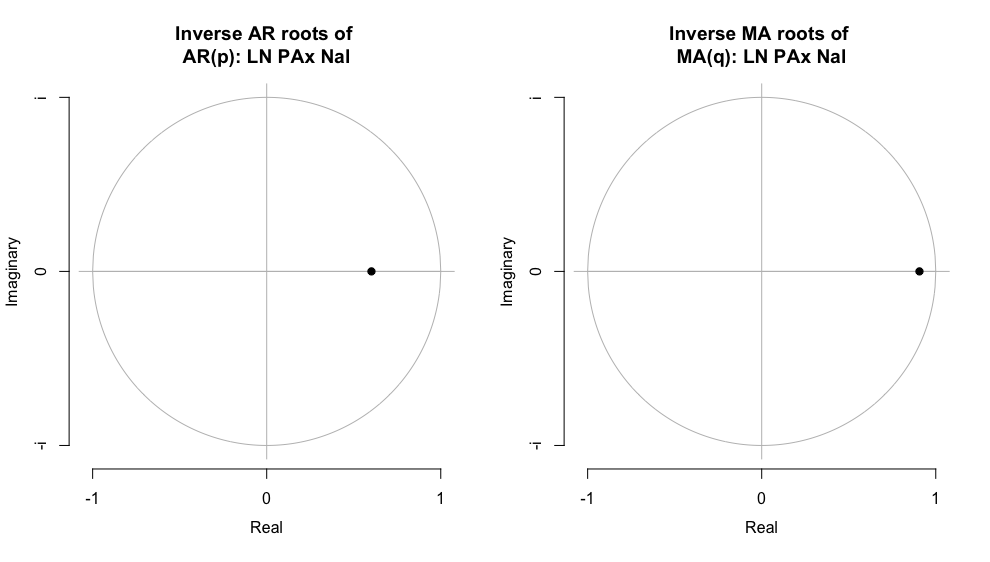
\includegraphics[width = 1.0 \textwidth]{Plots/G_Roots_ARMA11}
  \caption{Inveso de las Raíces del polinomio característico de un ARMA(1,1)}
  \label{G_Roots_ARMA11}
\end{figure}

\begin{figure}
\centering
    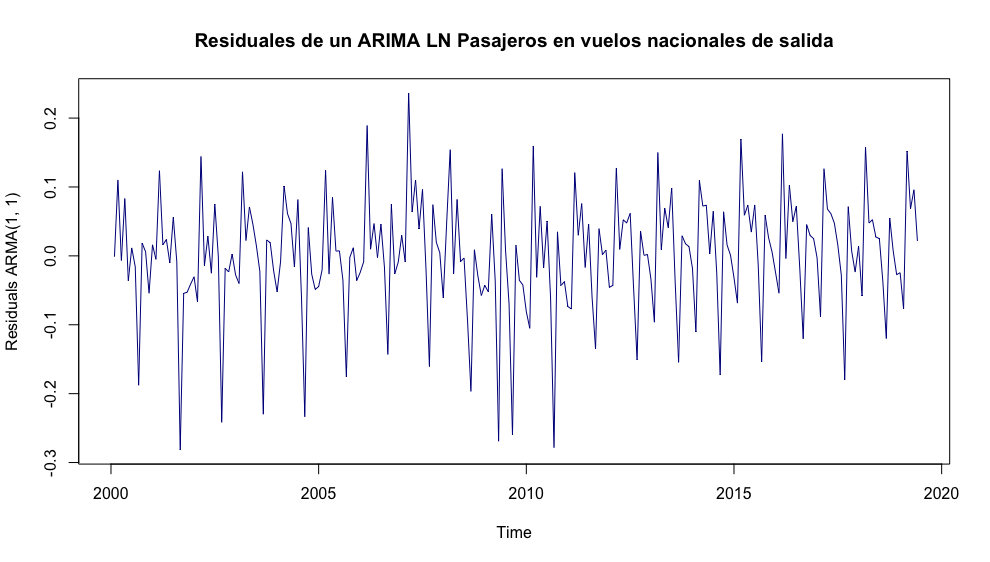
\includegraphics[width = 1.0 \textwidth]{Plots/G_Residuals_ARMA11}
    \caption{Residuales de un $ARMA(1, 1)$ de la serie $DLPaxNal_t$}
    \label{G_Residuals_ARMA11}
\end{figure}

En lo que resta de este capítulo, utilizaremos la serie en diferencias logarítmicas de los pasajeros en vuelos nacionales de salida, \(DLPaxNal_t\), para discutir los ejemplos que ilustran cada uno de los puntos teóricos que a continuación exponemos.

\hypertarget{funciuxf3n-de-autocorrelaciuxf3n-parcial}{%
\section{Función de Autocorrelación Parcial}\label{funciuxf3n-de-autocorrelaciuxf3n-parcial}}

Ahora introduciremos el concepto de Función de Autocorrelación Parcial (PACF, por sus siglas en inglés). Primero, dadas las condiciones de estabilidad y de convergencia, si suponemos que un proceso AR, MA, ARMA o ARIMA tienen toda la información de los rezagos de la serie en conjunto y toda la información de los promedio móviles del término de error, resulta importante construir una métrica para distinguir el efecto de \(X_{t - \tau}\) o el efecto de \(U_{t - \tau}\) (para cualquier \(\tau\)) sobre \(X_t\) de forma individual.

La idea es construir una métrica de la correlación que existe entre las diferentes varibles aleatorias, si para tal efecto se ha controlado el efecto del resto de la información. Así, podemos definir la ecuación que puede responder a este planteamiento como:
\begin{equation}
    X_t = \phi_{k1} X_{t-1} + \phi_{k2} X_{t-2} + \ldots + \phi_{kk} X_{t-k} + U_t
    \label{PACF_Eq}
\end{equation}

Donde \(\phi_{ki}\) es el coeficiente de la variable dada con el rezago \(i\) si el proceso tiene un órden \(k\). Así, los coeficientes \(\phi_{kk}\) son los coeficientes de la autocorrelación parcial (considerando un proceso AR(k)). Observemos que la autocorrelaicón parcial mide la correlación entre \(X_t\) y \(X_{t-k}\) que se mantiene cuando el efecto de las variables \(X_{t-1}\), \(X_{t-2}\), \(\ldots\) y \(X_{t-k-1}\) en \(X_{t}\) y \(X_{t-k}\) ha sido eliminado.

Dada la expresión considerada en la ecuación (\ref{PACF_Eq}), podemos resolver el problema de establecer el valor de cada \(\phi_{ki}\) mediante la solución del sistema que se representa en lo siguiente:
\begin{equation}
    \left[ 
    \begin{array}{c}
        \rho(1) \\
        \rho(2) \\
        \vdots \\
        \rho(k)
    \end{array} 
    \right]
    = 
    \left[ 
    \begin{array}{c c c c}
        1 & \rho(1) & \ldots & \rho(k - 1)\\
        \rho(1) & 1 & \ldots & \rho(k - 2)\\
        \rho(2) & \rho(1) & \ldots & \rho(k - 3)\\
        \vdots & \vdots & \ldots & \vdots\\
        \rho(k - 1) & \rho(k - 2) & \ldots & 1\\
    \end{array} 
    \right]
    \left[ 
    \begin{array}{c}
        \phi_{k1} \\
        \phi_{k2} \\
        \phi_{k3} \\
        \vdots \\
        \phi_{kk} \\
    \end{array} 
    \right]
\end{equation}

Del cual se puede derivar una solución, resoviendo por el método de cramer, o cualquier otro método que consideremos y que permita calcular la solución de sistemas de ecuaciones.

Posterior al análisis analítico platearemos un enfoque para interpretar las funciones de autocorrelación y autocorrelación parcial. Este enfoque pretende aportar al principio de parcimonia, en el cual podemos identificar el número de parámetros que posiblemente puede describir mejor a la serie en un modelo ARMA(p, q).

En el Cuadro \ref{ACF_PACF} se muestra un resumen de las caranterísticas que debemos observar para determinar el número de parámetros de cada uno de los componentes AR y MA. Lo anterior por observación de las funciones de autocorrelación y autocorrelación parcial. Este enfoque no es el más formal, más adelante implemtaremos uno más formal y que puede ser más claro de cómo determinar el númeto de parámetros.

\begin{table}
\centering
\begin{tabular}{| c | c | c |}
    \hline
    Modelo  & Función de Autocorrelación & Función de Autocorrelación \\
     si: &   & Parcial \\
    \hline
    MA(q) & Rompimienttos en la función & No hay rompimientos \\
    AR(p) & No hay rompimientos & Rompimienttos en la función \\
    \hline
    \end{tabular}
\caption{Relación entre la Función de Autocorrelación y la Función de Autocorrelación Parcial de una serie $X_t$.}
\label{ACF_PACF}
\end{table}

Continuando con el ejemplo en la Figura (\ref{G_ACF_PACF}) mostramos tanto la Función de Autocorrelación como la Función de Autocorrelación Parcial. En esta identificamos que ambas gráficas muestran que el modelo que explica a la variable \(DLPaxNal_t\) tiene tanto componentes AR como MA. Sin embargo, dado lo errático del comportamiento de ambas funciones, resulta complicado determinar cuál sería un buen número de parametros \(p\) y \(q\) a considerar en el \(ARMA(p,q)\). Por esta razón a continuación platearemos algunas pruebas más formales para determinar dichos parámetros.

\begin{figure}
  \centering
    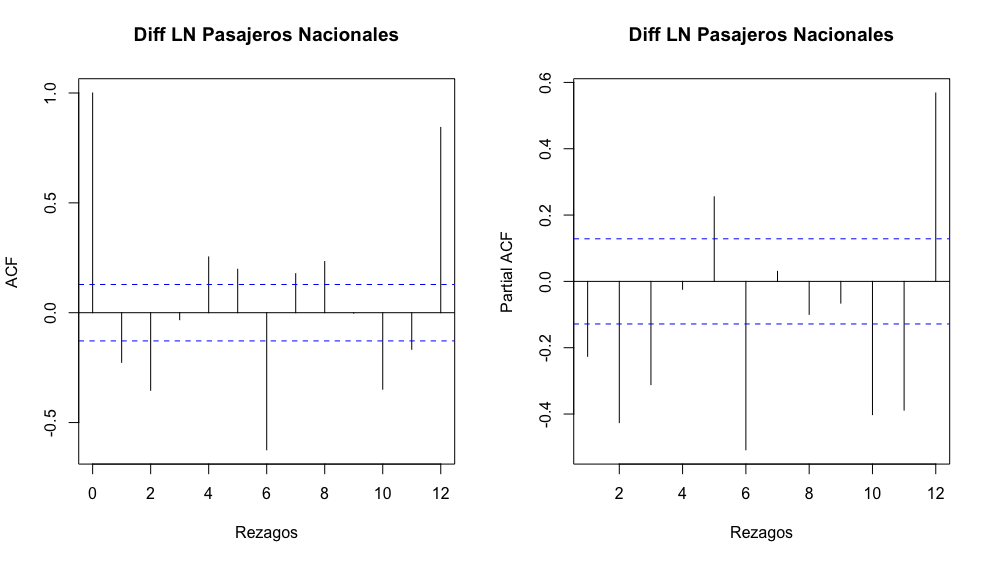
\includegraphics[width = 1.0 \textwidth]{Plots/G_ACF_PACF}
  \caption{Función de Autocorrelación y la Función de Autocorrelación Parcial de una serie $DLPaxNal_t$.}
  \label{G_ACF_PACF}
\end{figure}

\hypertarget{selecciuxf3n-de-las-constantes-p-q-d-en-un-arp-un-maq-un-armap-q-o-un-arimap-d-q}{%
\section{Selección de las constantes p, q, d en un AR(p), un MA(q), un ARMA(p, q) o un ARIMA(p, d, q)}\label{selecciuxf3n-de-las-constantes-p-q-d-en-un-arp-un-maq-un-armap-q-o-un-arimap-d-q}}

Respecto de cómo estimar un proceso ARMA(p, q) --en general utilizaremos este modelo para discutir, pero lo planteado en esta sección es igualmente aplicable en cualquier otro caso como aquellos modelos que incluyen variables exogénas-- existen diversas formas de estimar los paramétros \(a_i\) y \(b_i\): i) por máxima verosimilitd y ii) por mínimos cuadrados órdinarios. El primer caso requiere que conozcamos la distribución del proceso aleatorio \(U_t\). El segundo, por el contrario, no requiere el mismo supuesto. No obstante, para el curso utilizaremos el método de máxima verosimilitud.

Otra duda que debe quedar hasta el momento es ¿cómo determinar el orden \(p\) y \(q\) del proceso ARMA(p, q)? La manera más convencional y formal que existe para tal efecto es utilizar los criterios de información. Así, el orden se elije de acuerdo a aquel críterio de información que resulta ser el mínimo. En el caso de \(d\) se selecciona revisando la gráfica que parezca más estacionaria--más adelante mostraremos un proceso más formal para su selección.

Los criterios de información más comunes son los siguientes:

\begin{enumerate}
\item FPE (Final Prediction Error):
\begin{equation}
    FPE = \frac{T+m}{T-m}\frac{1}{T}\sum_{t=1}^{T} \left( \hat{U}_t^{(p)} \right) ^2
\end{equation}
\item Akaike:
\begin{equation}
    AIC = ln \left[ \frac{1}{T} \sum_{t=1}^{T} \left( \hat{U}_t^{(p)} \right) ^2 \right] + m \frac{2}{T}
\end{equation}
\item Schwarz:
\begin{equation}
    SC = ln \left[ \frac{1}{T} \sum_{t=1}^{T} \left( \hat{U}_t^{(p)} \right) ^2 \right] + m \frac{ln(T)}{T}
\end{equation}
\item Hannan - Quinn:
\begin{equation}
    HQ = ln \left[ \frac{1}{T} \sum_{t=1}^{T} \left( \hat{U}_t^{(p)} \right) ^2 \right] + m \frac{2 ln(ln(T))}{T}
\end{equation}
\end{enumerate}

Donde \(\hat{U}_t^{(p)}\) son los residuales estimados mediante un proceso ARIMA y \(m\) es el número de parametros estimados: \(m = p + q + 0 + 1\) (ya que asumimos que \(d = 0\)). Una propiedad que no se debe perder de vista es que los criterios de información cumplen la siguiente relación:
\begin{equation}
    orden(SC) \leq orden(HQ) \leq orden(AIC)
\end{equation}

Por esta razón, durante el curso solo utilizaremos el criterio se Akaike para determinar el orden óptimo del proceso ARMA, ya que ello garantiza el orden más grande posible.

Ahora veamos un ejemplo de estimación del número de rezagos optimo de un \(ARMA(p, q)\). Retomemos la serie en diferencias logarítmicas de los pasajeros en vuelos nacionales de salidas, pero ahora incluiremos la variables exógenas de dummies estacionales: enero, febrero, julio y diciembre.

Como mencionamos, las gráficas de las funciones de autocorrelación permiten observar el valor de la correlación existente entre la variable en el momento \(t\) con cada uno de los rezagos. Incluso la Función de Autocorrelación Parcial puede ayudar a determinar el número máximo de rezagos que se debe incluir en el proceso \(AR(p)\). No obstante, una métrica más formal es el uso de los criterios de información. En nuestro caso, dado lo discutido, sólo utilizareemos el criterio de Akaike.

Al respecto, en el Cuadro (\ref{Selec_ARMApq}) reportamos el criterio de Akaike que resultan de aplicar dicho criterio a los residuales resultantes de cada combinación de procesos \(ARMA(p, q)\). La forma de escoger será aquel modelo que reporta el criterio de Akaike menor. En la cuarta columna de la tabla se señala el valor del criterio de información que resulta ser el mínimo de todos los posibles.

\begin{table}
\centering
\begin{tabular}{|c | c | c | c | c |}
\hline
    Modelo & AR(p) & MA(p) & Akaike (AIC) & Óptimo \\
\hline
    1 & 1 & 1 & -475.1190 &  \\
    2 & 1 & 2 & -473.4397 &  \\
    3 & 1 & 3 & -483.1239 &  \\
    4 & 1 & 4 & -482.4932 &  \\
    5 & 1 & 5 & -506.9880 &  \\
    6 & 1 & 6 & -533.9411 &  \\
    7 & 2 & 1 & -473.4758 &  \\
    $\vdots$ & $\vdots$ & $\vdots$ & $\vdots$ & $\vdots$ \\
    24 & 4 & 6 & -752.8996 & * \\
    $\vdots$ & $\vdots$ & $\vdots$ & $\vdots$ & $\vdots$ \\
    36 & 6 & 6 & -752.2632 &  \\
\hline
\end{tabular}
\caption{Criterio de Akike para diferentes modelos $ARMA(p, q)$ de la serie $DLPaxNal_t$.}
\label{Selec_ARMApq}
\end{table}

El Cuadro (\ref{Selec_ARMApq}) reporta los resultados para 36 diferentes modelos, todos incluyen variables exogenas. Como resultado del análisis concluimos que el modelo más adecuado es el 24, el cual considera un \(ARMA(4, 6)\), con variables dummies para controlar la estacionalidad de los meses de enero, febrero, julio y diciembre. En el Cuadro (\ref{Result_ARMApq}) mostramos los resutados del modelo.

No obstante, una inspección de los residuales del modelo nos permite sospechar que requiere de incluir un par de dummies más. Ambas, asociadas con la caída del transporte aéreo en 2009, principalmente asociado con la crisis mundial de ese año. La Figura (\ref{G_Residuals_ARMA46}) muestra los residuales mencionados.

\begin{figure}
  \centering
    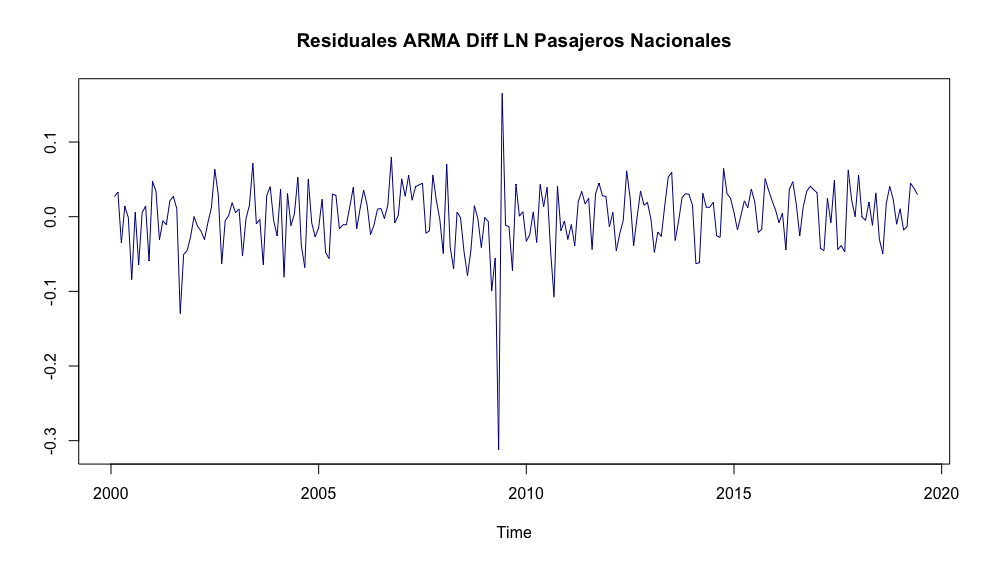
\includegraphics[width = 1.0 \textwidth]{Plots/G_Residuals_ARMA46}
  \caption{Residuales del ARMA(4, 6) de una serie $DLPaxNal_t$.}
  \label{G_Residuals_ARMA46}
\end{figure}

Una vez incluidas dos dummies más para mayo y junio de 2009, analizamos un total de 36 modelos ARMA y determinamos que el orden que minimizza el criterio de Akaike es un \(ARMA(4, 6)\). El Cuadro (\ref{Result_ARMApq}) muestra los resultados para este nuevo modelo. No lo motramos en esta sección, pero ambos modelos reportados tienen raices de sus respectivos polinomios característicos menores a 1 en valor absoluto. En la Figura \ref{G_Residuals_ARMA46_D} mostramos los residuales ahora ajustados por las dummies de mayo y junio de 2009.

\begin{table}
\centering
\begin{tabular}{|c | c | c | c | c |}
\hline
     & \multicolumn{2}{| c |}{Modelo 1} & \multicolumn{2}{| c |}{Modelo 2} \\
\hline
    Variable & Coeficiente & Error Est. & Coeficiente & Error Est. \\
\hline
    Constante & 0.0134 & 0.0033 & 0.0145 & 0.0029 \\
    $DLPaxNal_{t-1}$ & 0.0004 & 0.0011 & 0.0014 & 0.0016 \\
    $DLPaxNal_{t-2}$ & 0.9997 & 0.0019 & 0.9988 & 0.0024 \\
    $DLPaxNal_{t-3}$ & 0.0001 & 0.0012 & 0.0002 & 0.0014 \\
    $DLPaxNal_{t-4}$ & -0.9997 & 0.0004 & -0.9993 & 0.0009 \\
    $\hat{U}_{t-1}$ & -0.2877 & 0.0670 & -0.1472 & 0.0633 \\
    $\hat{U}_{t-2}$ & -1.2028 & 0.0608 & -1.3323 & 0.0625 \\
    $\hat{U}_{t-3}$ & 0.2302 & 0.0765 & 0.1201 & 0.0756 \\
    $\hat{U}_{t-4}$ & 1.2085 & 0.0645 & 1.3142 & 0.0642 \\
    $\hat{U}_{t-5}$ & -0.2634 & 0.0708 & -0.1034 & 0.0717 \\
    $\hat{U}_{t-6}$ & -0.2171 & 0.0606 & -0.3864 & 0.0657 \\
    $DEne_{t}$ & -0.2904 & 0.0172 & -0.2865 & 0.0156 \\
    $DFeb_{t}$ & -0.1312 & 0.0170 & -0.1273 & 0.0140 \\
    $DJul_{t}$ & 0.3303 & 0.0173 & 0.3164 & 0.0156 \\
    $Dic_{t}$ & -0.0118 & 0.0169 & -0.0138 & 0.0137 \\
    $DMay2009_{t}$ &   &   & -0.3378 & 0.0360 \\
    $DJun2009_{t}$ &   &   & 0.2371 & 0.0359 \\
\hline
    $\hat{\sigma}^2$ & 0.001841 &   & 0.001283 &  \\
    AIC & -752.9 &   & -835.73 &  \\
\hline
    \multicolumn{5}{ l }{Nota: El método de estimación fue máxima verosimilitud.} \\
\end{tabular}
\caption{Criterio de Akike para diferentes modelos ARMA(p, q) de la serie $DLPaxNal_t$.}
\label{Result_ARMApq}
\end{table}

\begin{figure}
  \centering
    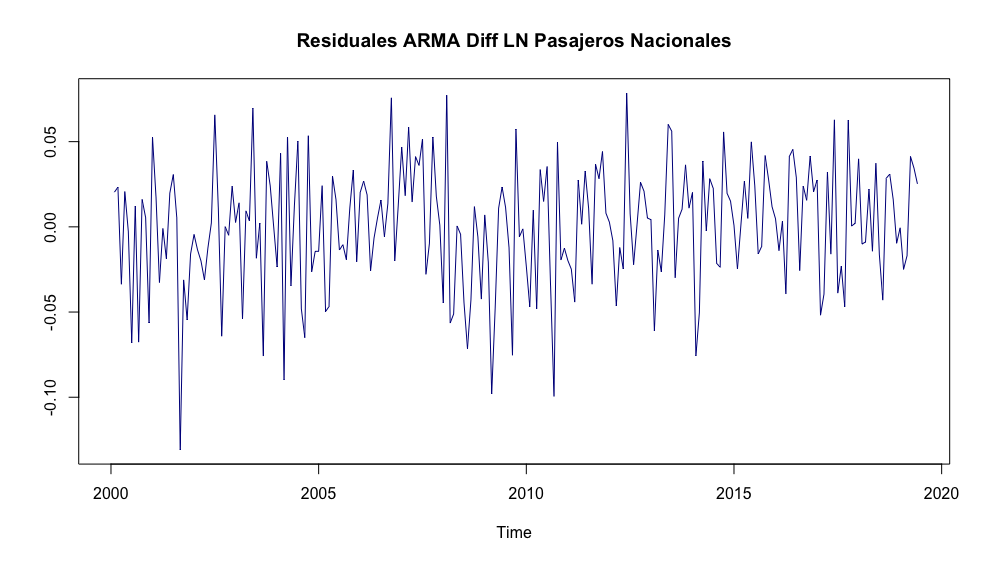
\includegraphics[width = 1.0 \textwidth]{Plots/G_Residuals_ARMA46_D}
  \caption{Residuales del ARMA(4, 6) de una serie $DLPaxNal_t$.}
  \label{G_Residuals_ARMA46_D}
\end{figure}

\hypertarget{pronuxf3sticos}{%
\section{Pronósticos}\label{pronuxf3sticos}}

Para pronósticar el valor de la serie es necesario determinar cuál es el valor esperado de la serie en un momento \(t + \tau\) condicional en que ésta se comporta como un \(AR(p)\), un \(MA(q)\) o un \(ARMA(p, q)\) y a que los valores antes de \(t\) están dados. Por lo que el pronóstico de la serie estará dado por una expresión:
\begin{eqnarray}
    \mathbb{E}_t[X_{t+\tau}] = \delta + a_1 \mathbb{E}_t[X_{t+\tau-1}] + a_2 \mathbb{E}_t[X_{t+\tau-2}] + \ldots + + a_p \mathbb{E}_t[X_{t+\tau-p}]
    \label{ARMApq_For}
\end{eqnarray}

Lo anterior para todo \(\tau = 0, 1, 2, \ldots\) y considerando que los componentes MA(q) en la eucación (\ref{ARMApq_For}) son cero dado que para todo valor \(t + \tau\) es cierto que \(\mathbb{E}_t[U_{t+\tau}]\).

Continuando con el ejemplo, en la Figura (\ref{fig:fig412}\}) mostramos el resultado del pronóstico de la serie a partir del modelo ARMA(4, 6) que hemos discutido anteriormente.

\begin{Shaded}
\begin{Highlighting}[]
\FunctionTok{library}\NormalTok{(ggplot2)}
\FunctionTok{library}\NormalTok{(dplyr)}
\FunctionTok{library}\NormalTok{(readxl)}
\FunctionTok{library}\NormalTok{(stats)}

\NormalTok{Datos }\OtherTok{\textless{}{-}} \FunctionTok{read\_excel}\NormalTok{(}\StringTok{"BD/Base\_Transporte\_ARIMA.xlsx"}\NormalTok{, }\AttributeTok{sheet =} \StringTok{"Datos"}\NormalTok{, }\AttributeTok{col\_names =} \ConstantTok{TRUE}\NormalTok{)}

\NormalTok{Pax\_Nal }\OtherTok{\textless{}{-}} \FunctionTok{ts}\NormalTok{(Datos}\SpecialCharTok{$}\NormalTok{Pax\_Nal, }
              \AttributeTok{start =} \FunctionTok{c}\NormalTok{(}\DecValTok{2000}\NormalTok{, }\DecValTok{1}\NormalTok{), }
              \AttributeTok{freq =} \DecValTok{12}\NormalTok{)}

\NormalTok{LPax\_Nal }\OtherTok{\textless{}{-}} \FunctionTok{ts}\NormalTok{(}\FunctionTok{log}\NormalTok{(Datos}\SpecialCharTok{$}\NormalTok{Pax\_Nal), }
               \AttributeTok{start =} \FunctionTok{c}\NormalTok{(}\DecValTok{2000}\NormalTok{, }\DecValTok{1}\NormalTok{), }
               \AttributeTok{freq =} \DecValTok{12}\NormalTok{)}

\NormalTok{DLPax\_Nal }\OtherTok{\textless{}{-}} \FunctionTok{ts}\NormalTok{(}\FunctionTok{log}\NormalTok{(Datos}\SpecialCharTok{$}\NormalTok{Pax\_Nal) }\SpecialCharTok{{-}} \FunctionTok{lag}\NormalTok{(}\FunctionTok{log}\NormalTok{(Datos}\SpecialCharTok{$}\NormalTok{Pax\_Nal), }\DecValTok{1}\NormalTok{),}
                \AttributeTok{start =} \FunctionTok{c}\NormalTok{(}\DecValTok{2000}\NormalTok{, }\DecValTok{1}\NormalTok{), }
                \AttributeTok{freq =} \DecValTok{12}\NormalTok{)}

\NormalTok{D\_Mar2020   }\OtherTok{\textless{}{-}} \FunctionTok{ts}\NormalTok{(Datos}\SpecialCharTok{$}\NormalTok{D\_Mar2020, }
                \AttributeTok{start =} \FunctionTok{c}\NormalTok{(}\DecValTok{2000}\NormalTok{, }\DecValTok{1}\NormalTok{), }
                \AttributeTok{freq =} \DecValTok{12}\NormalTok{)}

\NormalTok{D\_Abr2020   }\OtherTok{\textless{}{-}} \FunctionTok{ts}\NormalTok{(Datos}\SpecialCharTok{$}\NormalTok{D\_Abr2020, }
                \AttributeTok{start =} \FunctionTok{c}\NormalTok{(}\DecValTok{2000}\NormalTok{, }\DecValTok{1}\NormalTok{), }
                \AttributeTok{freq =} \DecValTok{12}\NormalTok{)}

\NormalTok{D\_Jun2020   }\OtherTok{\textless{}{-}} \FunctionTok{ts}\NormalTok{(Datos}\SpecialCharTok{$}\NormalTok{D\_Jun2020, }
                \AttributeTok{start =} \FunctionTok{c}\NormalTok{(}\DecValTok{2000}\NormalTok{, }\DecValTok{1}\NormalTok{), }
                \AttributeTok{freq =} \DecValTok{12}\NormalTok{)}

\NormalTok{D\_Jul2020 }\OtherTok{\textless{}{-}} \FunctionTok{ts}\NormalTok{(Datos}\SpecialCharTok{$}\NormalTok{D\_Jul2020, }
                \AttributeTok{start =} \FunctionTok{c}\NormalTok{(}\DecValTok{2000}\NormalTok{, }\DecValTok{1}\NormalTok{), }
                \AttributeTok{freq =} \DecValTok{12}\NormalTok{)}

\NormalTok{D\_Mar2021 }\OtherTok{\textless{}{-}} \FunctionTok{ts}\NormalTok{(Datos}\SpecialCharTok{$}\NormalTok{D\_Mar2021, }
                \AttributeTok{start =} \FunctionTok{c}\NormalTok{(}\DecValTok{2000}\NormalTok{, }\DecValTok{1}\NormalTok{), }
                \AttributeTok{freq =} \DecValTok{12}\NormalTok{)}

\NormalTok{D\_Ene }\OtherTok{\textless{}{-}} \FunctionTok{ts}\NormalTok{(Datos}\SpecialCharTok{$}\NormalTok{D\_Ene, }
            \AttributeTok{start =} \FunctionTok{c}\NormalTok{(}\DecValTok{2000}\NormalTok{, }\DecValTok{1}\NormalTok{), }
            \AttributeTok{freq =} \DecValTok{12}\NormalTok{)}

\NormalTok{D\_Feb }\OtherTok{\textless{}{-}} \FunctionTok{ts}\NormalTok{(Datos}\SpecialCharTok{$}\NormalTok{D\_Feb, }
            \AttributeTok{start =} \FunctionTok{c}\NormalTok{(}\DecValTok{2000}\NormalTok{, }\DecValTok{1}\NormalTok{), }
            \AttributeTok{freq =} \DecValTok{12}\NormalTok{)}

\NormalTok{D\_Jul }\OtherTok{\textless{}{-}} \FunctionTok{ts}\NormalTok{(Datos}\SpecialCharTok{$}\NormalTok{D\_Jul, }
            \AttributeTok{start =} \FunctionTok{c}\NormalTok{(}\DecValTok{2000}\NormalTok{, }\DecValTok{1}\NormalTok{), }
            \AttributeTok{freq =} \DecValTok{12}\NormalTok{)}

\NormalTok{D\_Dic }\OtherTok{\textless{}{-}} \FunctionTok{ts}\NormalTok{(Datos}\SpecialCharTok{$}\NormalTok{D\_Dic, }
            \AttributeTok{start =} \FunctionTok{c}\NormalTok{(}\DecValTok{2000}\NormalTok{, }\DecValTok{1}\NormalTok{), }
            \AttributeTok{freq =} \DecValTok{12}\NormalTok{)}

\NormalTok{ARMA\_Ex\_DLPax\_Nal\_2 }\OtherTok{\textless{}{-}} \FunctionTok{arima}\NormalTok{(DLPax\_Nal, }\AttributeTok{order =} \FunctionTok{c}\NormalTok{(}\DecValTok{6}\NormalTok{, }\DecValTok{0}\NormalTok{, }\DecValTok{6}\NormalTok{),}
                             \AttributeTok{xreg =} \FunctionTok{cbind}\NormalTok{(D\_Ene, D\_Feb, D\_Jul, D\_Dic, D\_Mar2020, D\_Abr2020, D\_Jun2020, D\_Jul2020, D\_Mar2021),}
                             \AttributeTok{method =} \StringTok{"ML"}\NormalTok{)}
\end{Highlighting}
\end{Shaded}

\begin{verbatim}
## Warning in arima(DLPax_Nal, order = c(6, 0, 6), xreg = cbind(D_Ene, D_Feb, :
## possible convergence problem: optim gave code = 1
\end{verbatim}

\begin{Shaded}
\begin{Highlighting}[]
\NormalTok{Predict\_Datos }\OtherTok{\textless{}{-}} \FunctionTok{read\_excel}\NormalTok{(}\StringTok{"BD/Predict\_Base\_Transporte\_ARIMA.xlsx"}\NormalTok{, }\AttributeTok{sheet =} \StringTok{"Datos"}\NormalTok{, }\AttributeTok{col\_names =} \ConstantTok{TRUE}\NormalTok{)}

\NormalTok{D\_Mar2020\_f }\OtherTok{\textless{}{-}} \FunctionTok{ts}\NormalTok{(Predict\_Datos}\SpecialCharTok{$}\NormalTok{D\_Mar2020, }
                \AttributeTok{start =} \FunctionTok{c}\NormalTok{(}\DecValTok{2022}\NormalTok{, }\DecValTok{7}\NormalTok{), }
                \AttributeTok{freq =} \DecValTok{12}\NormalTok{)}

\NormalTok{D\_Abr2020\_f }\OtherTok{\textless{}{-}} \FunctionTok{ts}\NormalTok{(Predict\_Datos}\SpecialCharTok{$}\NormalTok{D\_Abr2020, }
                \AttributeTok{start =} \FunctionTok{c}\NormalTok{(}\DecValTok{2022}\NormalTok{, }\DecValTok{7}\NormalTok{), }
                \AttributeTok{freq =} \DecValTok{12}\NormalTok{)}

\NormalTok{D\_Jun2020\_f }\OtherTok{\textless{}{-}} \FunctionTok{ts}\NormalTok{(Predict\_Datos}\SpecialCharTok{$}\NormalTok{D\_Jun2020, }
                \AttributeTok{start =} \FunctionTok{c}\NormalTok{(}\DecValTok{2022}\NormalTok{, }\DecValTok{7}\NormalTok{), }
                \AttributeTok{freq =} \DecValTok{12}\NormalTok{)}

\NormalTok{D\_Jul2020\_f }\OtherTok{\textless{}{-}} \FunctionTok{ts}\NormalTok{(Predict\_Datos}\SpecialCharTok{$}\NormalTok{D\_Jul2020, }
                \AttributeTok{start =} \FunctionTok{c}\NormalTok{(}\DecValTok{2022}\NormalTok{, }\DecValTok{7}\NormalTok{), }
                \AttributeTok{freq =} \DecValTok{12}\NormalTok{)}

\NormalTok{D\_Mar2021\_f }\OtherTok{\textless{}{-}} \FunctionTok{ts}\NormalTok{(Predict\_Datos}\SpecialCharTok{$}\NormalTok{D\_Mar2021, }
                \AttributeTok{start =} \FunctionTok{c}\NormalTok{(}\DecValTok{2022}\NormalTok{, }\DecValTok{7}\NormalTok{), }
                \AttributeTok{freq =} \DecValTok{12}\NormalTok{)}

\NormalTok{D\_Ene\_f }\OtherTok{\textless{}{-}} \FunctionTok{ts}\NormalTok{(Predict\_Datos}\SpecialCharTok{$}\NormalTok{D\_Ene, }
            \AttributeTok{start =} \FunctionTok{c}\NormalTok{(}\DecValTok{2022}\NormalTok{, }\DecValTok{7}\NormalTok{), }
            \AttributeTok{freq =} \DecValTok{12}\NormalTok{)}

\NormalTok{D\_Feb\_f }\OtherTok{\textless{}{-}} \FunctionTok{ts}\NormalTok{(Predict\_Datos}\SpecialCharTok{$}\NormalTok{D\_Feb, }
            \AttributeTok{start =} \FunctionTok{c}\NormalTok{(}\DecValTok{2022}\NormalTok{, }\DecValTok{7}\NormalTok{), }
            \AttributeTok{freq =} \DecValTok{12}\NormalTok{)}

\NormalTok{D\_Jul\_f }\OtherTok{\textless{}{-}} \FunctionTok{ts}\NormalTok{(Predict\_Datos}\SpecialCharTok{$}\NormalTok{D\_Jul, }
           \AttributeTok{start =} \FunctionTok{c}\NormalTok{(}\DecValTok{2022}\NormalTok{, }\DecValTok{7}\NormalTok{), }
            \AttributeTok{freq =} \DecValTok{12}\NormalTok{)}

\NormalTok{D\_Dic\_f }\OtherTok{\textless{}{-}} \FunctionTok{ts}\NormalTok{(Predict\_Datos}\SpecialCharTok{$}\NormalTok{D\_Dic, }
            \AttributeTok{start =} \FunctionTok{c}\NormalTok{(}\DecValTok{2022}\NormalTok{, }\DecValTok{7}\NormalTok{), }
            \AttributeTok{freq =} \DecValTok{12}\NormalTok{)}

\NormalTok{DLPax\_Nal\_f }\OtherTok{\textless{}{-}} \FunctionTok{predict}\NormalTok{(ARMA\_Ex\_DLPax\_Nal\_2, }\AttributeTok{n.ahead =} \DecValTok{24}\NormalTok{, }
                      \AttributeTok{newxreg =} \FunctionTok{cbind}\NormalTok{(D\_Ene\_f, D\_Feb\_f, D\_Jul\_f, D\_Dic\_f, }
\NormalTok{                                      D\_Mar2020\_f, D\_Abr2020\_f, D\_Jun2020\_f, D\_Jul2020\_f, D\_Mar2021\_f))}

\NormalTok{Pronostico\_Arima }\OtherTok{\textless{}{-}} \FunctionTok{read\_excel}\NormalTok{(}\StringTok{"BD/Pronostico\_Arima.xlsx"}\NormalTok{, }\AttributeTok{sheet =} \StringTok{"Datos"}\NormalTok{, }\AttributeTok{col\_names =} \ConstantTok{TRUE}\NormalTok{)}

\NormalTok{Pronostico\_Arima}\SpecialCharTok{$}\NormalTok{Pax\_Nal\_f }\OtherTok{\textless{}{-}}\NormalTok{ Pronostico\_Arima}\SpecialCharTok{$}\NormalTok{Pax\_Nal}

\ControlFlowTok{for}\NormalTok{(i }\ControlFlowTok{in} \DecValTok{1}\SpecialCharTok{:}\DecValTok{24}\NormalTok{)\{}
\NormalTok{  Pronostico\_Arima}\SpecialCharTok{$}\NormalTok{Pax\_Nal\_f[}\DecValTok{281} \SpecialCharTok{+}\NormalTok{ i] }\OtherTok{\textless{}{-}} 
\NormalTok{    Pronostico\_Arima}\SpecialCharTok{$}\NormalTok{Pax\_Nal\_f[}\DecValTok{281} \SpecialCharTok{+}\NormalTok{ i }\SpecialCharTok{{-}} \DecValTok{1}\NormalTok{]}\SpecialCharTok{*}\NormalTok{(}\DecValTok{1} \SpecialCharTok{+}\NormalTok{ DLPax\_Nal\_f}\SpecialCharTok{$}\NormalTok{pred[i])}
\NormalTok{\}}

\FunctionTok{options}\NormalTok{(}\AttributeTok{scipen =} \DecValTok{999}\NormalTok{) }\CommentTok{\# NO notacion cientifica}

\FunctionTok{ggplot}\NormalTok{(}\AttributeTok{data =}\NormalTok{ Pronostico\_Arima, }\FunctionTok{aes}\NormalTok{(}\AttributeTok{x =}\NormalTok{ Periodo)) }\SpecialCharTok{+}
  \FunctionTok{geom\_line}\NormalTok{(}\FunctionTok{aes}\NormalTok{(}\AttributeTok{y =}\NormalTok{ Pax\_Nal\_f, }\AttributeTok{color =} \StringTok{"Pax\_Nal\_f"}\NormalTok{)) }\SpecialCharTok{+}
  \FunctionTok{geom\_line}\NormalTok{(}\FunctionTok{aes}\NormalTok{(}\AttributeTok{y =}\NormalTok{ Pax\_Nal, }\AttributeTok{color =} \StringTok{"Pax\_Nal"}\NormalTok{)) }\SpecialCharTok{+}
  \FunctionTok{scale\_color\_brewer}\NormalTok{(}\AttributeTok{type =} \StringTok{"qual"}\NormalTok{, }\AttributeTok{palette =} \DecValTok{2}\NormalTok{) }\SpecialCharTok{+}
  \CommentTok{\#theme\_bw() + }
  \FunctionTok{theme}\NormalTok{(}\AttributeTok{legend.position =} \StringTok{"bottom"}\NormalTok{) }\SpecialCharTok{+}
  \FunctionTok{theme}\NormalTok{(}\AttributeTok{legend.title =} \FunctionTok{element\_blank}\NormalTok{()) }\SpecialCharTok{+}
  \FunctionTok{guides}\NormalTok{(}\AttributeTok{col =} \FunctionTok{guide\_legend}\NormalTok{(}\AttributeTok{nrow =} \DecValTok{1}\NormalTok{, }\AttributeTok{byrow =} \ConstantTok{TRUE}\NormalTok{)) }\SpecialCharTok{+} 
  \FunctionTok{xlab}\NormalTok{(}\StringTok{"Tiempo"}\NormalTok{) }\SpecialCharTok{+} 
  \FunctionTok{ylab}\NormalTok{(}\StringTok{"Pasajeros"}\NormalTok{) }\SpecialCharTok{+} 
  \FunctionTok{theme}\NormalTok{(}\AttributeTok{plot.title =} \FunctionTok{element\_text}\NormalTok{(}\AttributeTok{size =} \DecValTok{11}\NormalTok{, }\AttributeTok{face =} \StringTok{"bold"}\NormalTok{, }\AttributeTok{hjust =} \DecValTok{0}\NormalTok{)) }\SpecialCharTok{+} 
  \FunctionTok{theme}\NormalTok{(}\AttributeTok{plot.subtitle =} \FunctionTok{element\_text}\NormalTok{(}\AttributeTok{size =} \DecValTok{10}\NormalTok{, }\AttributeTok{hjust =} \DecValTok{0}\NormalTok{)) }\SpecialCharTok{+} 
  \FunctionTok{theme}\NormalTok{(}\AttributeTok{plot.caption =} \FunctionTok{element\_text}\NormalTok{(}\AttributeTok{size =} \DecValTok{10}\NormalTok{, }\AttributeTok{hjust =} \DecValTok{0}\NormalTok{)) }\SpecialCharTok{+}
  \FunctionTok{theme}\NormalTok{(}\AttributeTok{plot.margin =} \FunctionTok{unit}\NormalTok{(}\FunctionTok{c}\NormalTok{(}\DecValTok{1}\NormalTok{,}\DecValTok{1}\NormalTok{,}\DecValTok{1}\NormalTok{,}\DecValTok{1}\NormalTok{), }\StringTok{"cm"}\NormalTok{)) }\SpecialCharTok{+}
  \FunctionTok{labs}\NormalTok{(}
    \AttributeTok{title =} \StringTok{"Pasajeros en vuelos nacionales (Salidas)"}\NormalTok{,}
    \AttributeTok{subtitle =} \StringTok{"(Ene{-}2000 a Jun{-}2019)"}\NormalTok{,}
    \AttributeTok{caption =} \StringTok{"Fuente: Elaboración propia"}
\NormalTok{  )}
\end{Highlighting}
\end{Shaded}

\begin{verbatim}
## Warning: Removed 24 rows containing missing values (`geom_line()`).
\end{verbatim}

\begin{figure}

{\centering 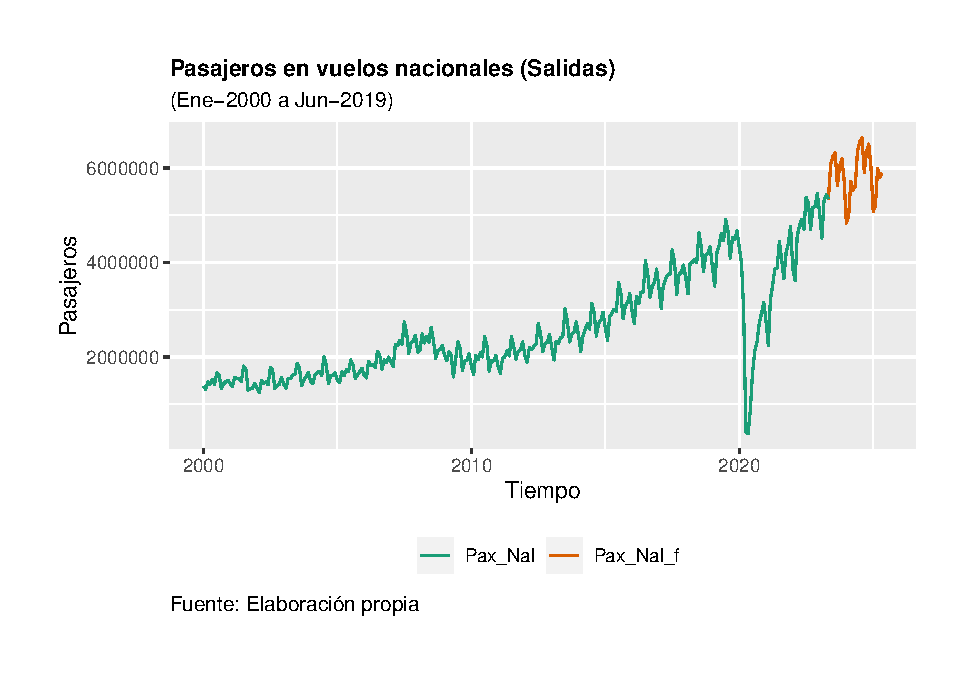
\includegraphics{Notas-Series-Tiempo_files/figure-latex/fig412-1} 

}

\caption{Pronóstico de la serie $PaxNAl_t$ a partir de una ARMA(4,6) en diferencias logaritmicas}\label{fig:fig412}
\end{figure}

\begin{Shaded}
\begin{Highlighting}[]
\FunctionTok{ggsave}\NormalTok{(}\StringTok{"Pax\_Nal\_f.png"}\NormalTok{, }\AttributeTok{width =} \DecValTok{20}\NormalTok{, }\AttributeTok{height =} \DecValTok{15}\NormalTok{, }\AttributeTok{units =} \StringTok{"cm"}\NormalTok{)}
\end{Highlighting}
\end{Shaded}

\begin{verbatim}
## Warning: Removed 24 rows containing missing values (`geom_line()`).
\end{verbatim}

  \bibliography{book.bib,packages.bib}

\end{document}
